% Williams Physics Thesis template
% Patterned after the work of Cole Meisenhelder '15
% Commented by Prof. Charlie Doret, 12/2016

\documentclass[12pt, oneside]{book} 

%\usepackage{fontspec}
%\setmainfont{Comic Sans MS}

% The \usepackage{} command will import predefined fonts, symbols, environments, etc.  For example, the ams packages below come from the American Mathematical Society and include all kinds of useful math symbols like integrals
\usepackage{amscd}
\usepackage{amsmath}
\usepackage{amssymb}
\usepackage{amsthm}
\usepackage{verbatim}
\usepackage[utf8]{inputenc}
\usepackage{geometry}
\usepackage{gensymb}                		% See geometry.pdf to learn the layout options. There are lots.
\geometry{letterpaper}                   		% ... or a4paper or a5paper or ... 
%\geometry{landscape}                		% Activate for for rotated page geometry
\usepackage[pdftex]{graphicx}				% Use pdf, png, jpg, or eps� with pdflatex;  change to xlatex if you want comic sans...   use eps in DVI mode	


%Added for chem figs
\usepackage{chemfig}
\usepackage{sidecap}
\usepackage[colorinlistoftodos]{todonotes}



\usepackage{setspace}
\usepackage{physics}
%\usepackage{subcaption}
\usepackage[numbers]{natbib}
\usepackage{pdfpages}
\usepackage{bm}
\usepackage{wrapfig}				% enables the use of \wrapfig, for figures with text wrapped around them
%\usepackage{lipsum}			% gives access to \lipsum, which dumps some latin text into your document as filler if you want to check formatting

%\usepackage[parfill]{parskip}    		% Activate to begin paragraphs with an empty line rather than an indent



% Here we set the page dimensions to match the standard thesis format.  These values should not be changed.
%%% SET LENTGH AND WIDTH %%%
\setlength{\textwidth}{6.5in}
\setlength{\textheight}{8.5in}
\setlength{\oddsidemargin}{0pt}
\setlength{\evensidemargin}{0pt}
\setlength{\topmargin}{0pt}
\setlength{\marginparsep}{0pt}
\setlength{\marginparwidth}{1in}


\usepackage{hyperref} %Makes clickable T.o.c.
\hypersetup{
	colorlinks=true, %set true if you want colored links
	linktoc=all,     %set to all if you want both sections and subsections linked
	allcolors = black %get rid of weird auto link highlighting
}
\usepackage[export]{adjustbox}


%\begin{document} starts LaTeX looking for actual content.  Everything above this point is purely formatting.
\begin{document}

\begin{titlepage}
\begin{center}

% \vspace* creates some vertical white space on the page to make the title page look more pleasing.  \vspace would do much the same thing, but would not insert the white space if we were at the top of a fresh page.  As this is the start of the document we're obviously at the beginning of a page, so the asterisk is necessary to ensure we still put in two cm of white space.
%\vspace*{2cm}
\vspace*{.5cm}

{\huge Toward An Adhesion Based Measurement of \\\vspace{.4em} Strain-Dependent Surface Stress in Soft Solids} % \huge sets the font size.  Other options include things like \large, \Large, \small, \tiny, etc.

\vspace{2cm}

{\large by\\\vspace{.25em}Jeremy K. Thaller}

\vspace{2cm}
{Professor Katharine E. Jensen, Advisor}

\begin{figure}[h]
	\vspace{.5cm}
	\centering
	
\includegraphics[width=.25\textwidth]{Chapters/Figures/seal.PNG}
\end{figure}  

% \vfill creates an arbitrary amount of vertical white space as necessary to fill the page
\vfill

A thesis submitted in partial fulfillment\\
of the requirements for the\\
Degree of Bachelor of Arts with Honors\\
in Physics

\vspace*{3cm}

WILLIAMS COLLEGE\\
Williamstown, Massachusetts\\
\today % you might choose to set a permanent date, but \today will put in today's date
\end{center}
\end{titlepage}

% \frontmatter defines the pieces of the thesis which will use roman numerals for page numbering
\frontmatter 


% \chapter{} and/or \chapter*{} will create a chapter in your thesis.  Including the asterisk will cause the chapter to not appear in the table of contents.

% \input will reference a particular .tex file.  Here we are grabbing a file entitled Abstract stored in the folder Chapters
\chapter{Abstract}
% Here is where you'll include the actual text for your abstract.  Because this lives inside the main document and will be included with a \input command, no tags are needed to start a new document.  Instead, just type.


%Your abstract will summarize your thesis in one or two paragraphs.  This brief summary should emphasize methods and results, not introductory material.

Surface stress, or surface tension, is a fundamental material property of interfaces. However, our understanding of solid surface tension and how it changes with deformation remains limited because it is difficult to measure in traditional stiff materials. Soft materials, including gels, provide a unique opportunity to measure these fundamental properties because they can be stretched elastically to very large strains. In this thesis, we have developed a new, adhesion-based approach to measure the solid surface stress of compliant materials as a function of applied strain. We measure the spontaneous indentation depth as a function of radius for rigid spheres adherered to compliant, sticky substrates, then fit the results to theory to obtain the surface stress, $ \Upsilon $ and adhesion energy, $ W $. By subsequently stretching the substrates biaxially and repeating the experiment, we obtain $ \Upsilon $ and $ W $ as a function of strain, $ \epsilon $. This approach is applicable to a wide range of soft materials. In this thesis, we report preliminary measurements for two types of polydimethylsiloxane (PDMS). 
\chapter{Executive Summary}
% Here we have your executive summary.
This thesis describes a new method for measuring strain dependent surface stress in soft solids, as well as the corresponding measurements for two silicone polymer gels. Over the past several years, recent attempts to measure surface stress in gels have returned a cornucopia of conflicting results, differing significantly in similar materials. Recently, Xu, Jensen et al. suggested that this discrepancy is an artifact of the strain state of the gels, and made the first measurement of strain-dependent surface stress, $\Upsilon(\epsilon)$, in solids \cite{xu2017direct}. In this paper, the authors reported that the surface stress changed dramatically under applied strain. At 18\% strain, the surface stress more than doubled. 
\begin{figure}[h!]
	\centering
%	\textbf{Should I give it a title?}\par\medskip
	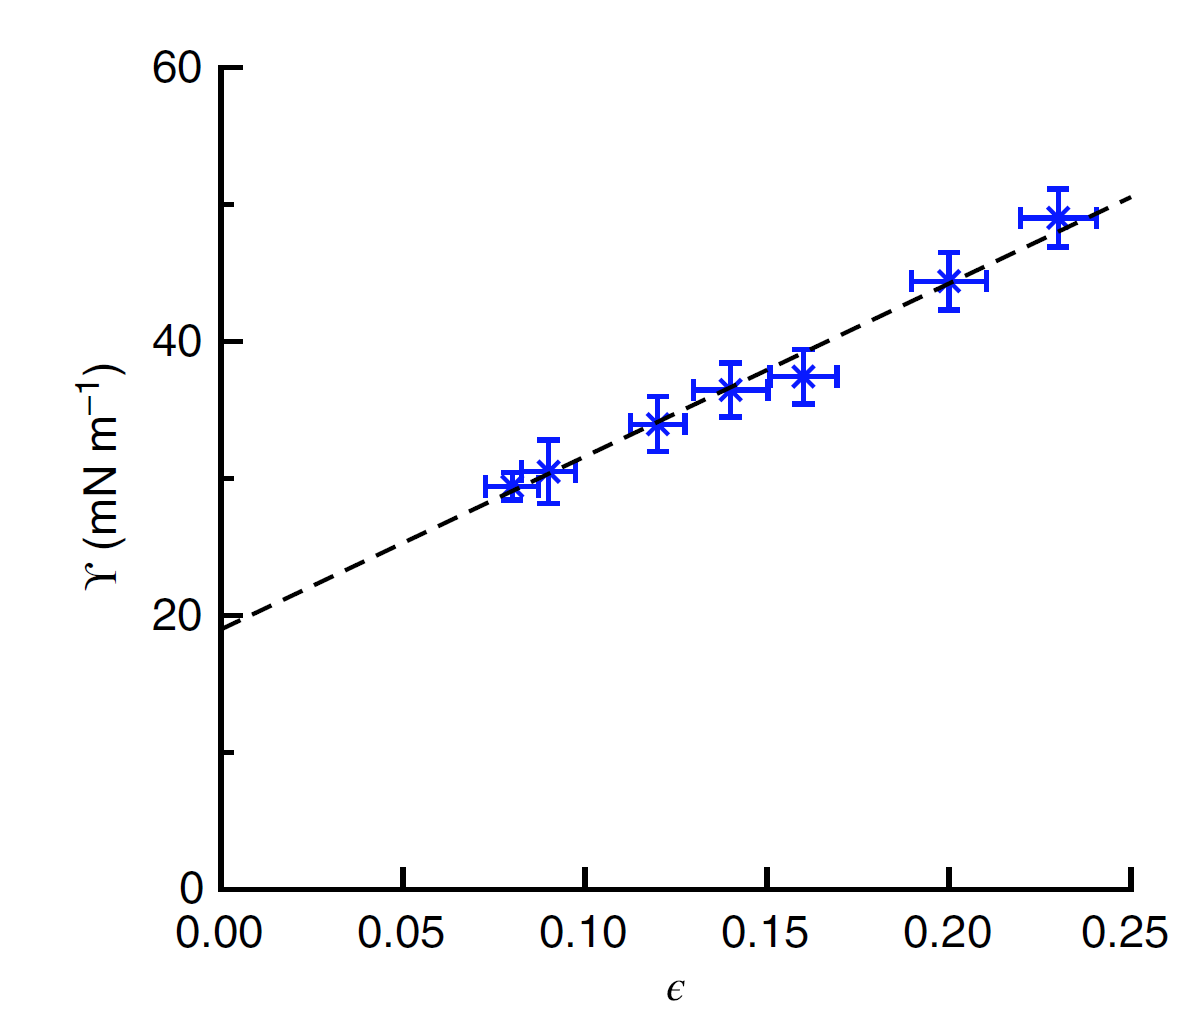
\includegraphics[width=0.7\linewidth]{Chapters/Figures/2017natcomfig}
	\caption[Surface Stress vs. Strain in Silicone]{This is first direct measurement of strain dependent surface stress in solids \cite{xu2017direct}. Using a compliant silicone gel, surface stress, $\Upsilon$, was found to grow linearly as a function of strain, $ \epsilon $.}
	\label{fig:2017natcomfig}
\end{figure}

Over the past year, we have helped develop a new method for measuring $\Upsilon(\epsilon)$ in soft solids. Our adhesion-based technique can be applied to a wide variety of stretchable materials. Additionally, we have build our own equibiaxial stretching apparatus, improving upon the earlier published design \cite{xu2017direct} to produce nearly twice the strain in identical materials. Using this technique we have measured the adhesion energy and surface stress in two types of silicone, as well as preliminary $ \Upsilon(\epsilon) $ measurements as we work towards recreate the controversial 2017 measurement.

Our results suggest that the surface tension in gels does significantly change under strain. The figure below is an example of how you can visually see this change for a single silica sphere sitting in a silicone substrate. As the underlying gel is stretched, the surface tension increases, reducing the depth into which the sphere sits. 
\begin{figure}[h!]
	\centering
	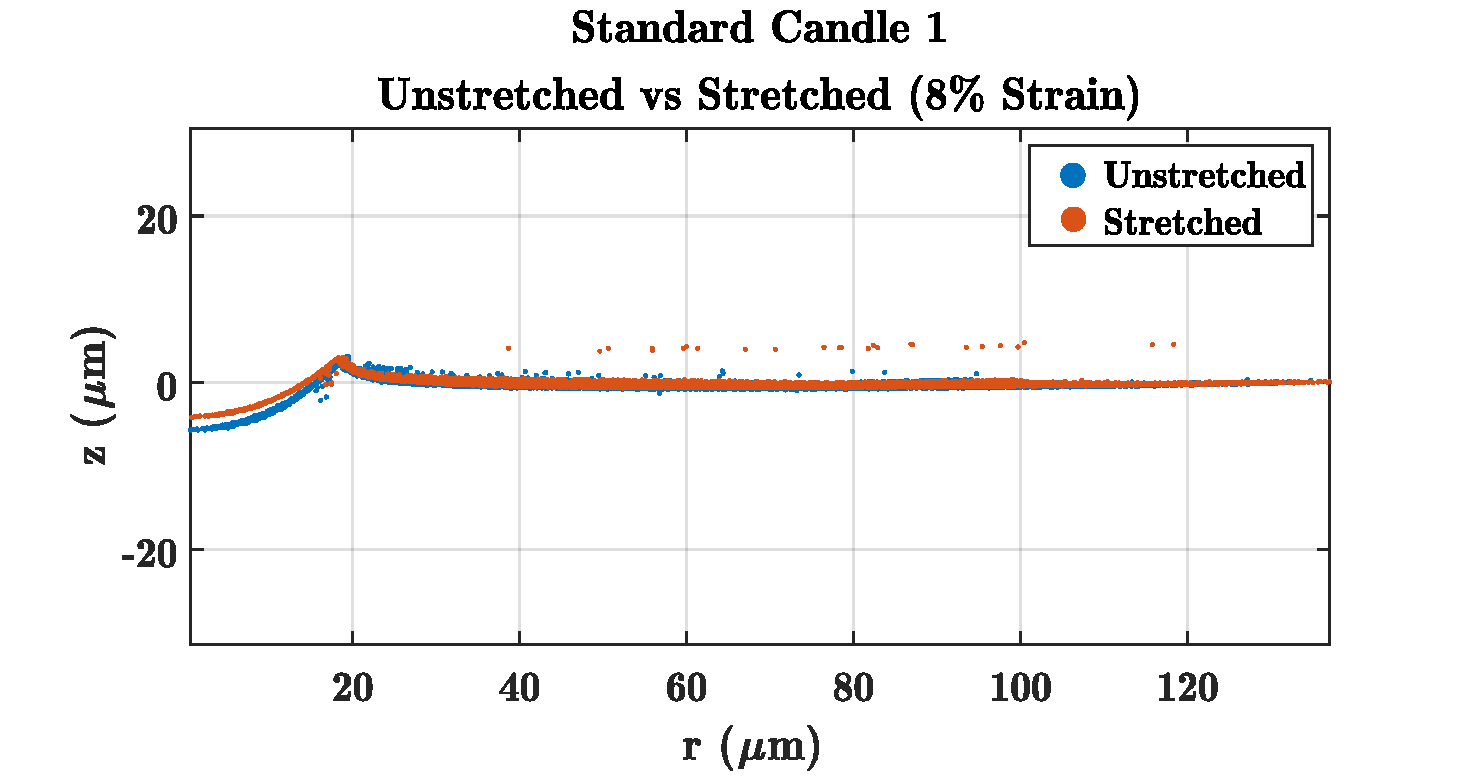
\includegraphics[width=\linewidth]{Chapters/Figures/sc1_unstretched_v_8ml}
	\caption[Side Collapse Comparison]{The side profile of the same silica sphere sitting in a silicone substrate before and after stretch. When a strain is applied, the sphere's indentation into the substrate is shallower. Substrate is Gelest PDMS with stiffness $\text{E}=6.3$ kPa.}	
	\label{fig:sc1unstretchedv8ml}
\end{figure}

\todo[inline, color=yellow]{I will continue to update this section. I hope to have a much more compelling graph to share, one more similar to Figure 1.}

%From Charlie:
%Your executive summary will give a detailed summary of your thesis, hitting the high points and perhaps including a figure or two.  This should have all of the important take-home messages; though details will of course be left for the thesis itself, here you should give enough detail for a reader to have a good idea of the content of the full document.  Importantly, this summary should be able to stand alone, separate from the rest of the document, so although you will be emphasizing the key results of your work, you will probably also want to include a sentence or two of introduction and context for the work you have done.




\chapter{Acknowledgements}
% Here we have a section where you might choose to acknoweldge your family, fellow students, advisor, dog, etc.

I would like to begin first and foremost by thanking my advisor (und Doktormutter), Professor Kate Jensen. She has had an incredibly positive impact on my life and influenced my trajectory after Williams more than anyone else. For that, I am eternally grateful and feel incredible fortunate to have been able work with her throughout the year. I also want to thank my friend and esteemed colleague Felix Knollmann, whose dedication to his own thesis helped encourage me to produce my best (read: most aesthetically pleasing) work and refrain from the procrastination that plagues any long term project. Next year I'll be perusing a graduate degree in materials science in Germany, a path I never would even have considered were it not for Felix and Kate. 

I also would like to thank my friends that have made my time at Williams such an enjoyable experience. From tubing down the Hoosic river with Sarah Ritzmann, to making soap with Marshall Borrus, to riding tandem bikes with Lucas Estrada, I'm blessed to have filled my (scarce) free-time with such bizarre and memorable experiences. That lack of free time is in part a result of my career on the track. I want to thank my coaches and teammates who have made these last four years such an incredible experience. Specifically, I want to thank coach Hoey and coach Barron, who may have taught me more about life than running itself. 

I would also like to thank my labmates, especially Josh Kang, who taught me both how to cure silicone and analyze it. It's been a pleasure working with Abdullah Nasir over the years. We first met while working together in Professor Majumder's lab, and I look forward to reading his thesis next year (probably written in crayon). Further, I really appreciate all the engineering help from Michael Taylor and Jason Mativi. Without them, this thesis would not have been possible.

Lastly, I would like to thank my parents. For raising me to always be curious, allowing me to attend Williams, and always supporting me in whatever ways they can, I am extremely grateful and fortunate. 




%\tableofcontents will create a table of contents.  By default it will include entries for any \chapter, \section, and \subsection command that appears in your thesis unless you have called the tag with an asterisk
\tableofcontents

\listoffigures

% \mainmatter defines the main body of the thesis and marks where regular numbering will begin
\mainmatter

\chapter{Introduction}
%The introduction is one of the most important pieces of your thesis.  Here is a place for you to introduce the problem(s) on which you have worked and place them in the larger context of your field.  You should aim to ensure that this section is completely understandable to virtually anyone - and certainly anyone with a sophomore-level grasp of physics.  Presumably this will include references to the literature.

%In addition to setting your work into context, a second good idea for your introduction is to give a short outline for what the rest of your thesis will discuss.  This is often done in the closing paragraph(s) of the introduction with sentences like ``In the following chapters \ldots " and ``Chapter 2 discusses \ldots"  Tremendous detail is not required in this outline, but rather just a brief road map for the rest of the document.

\section{Motivations}
Soft Condensed Matter Physics includes the study of colloids, liquid crystals, polymers, complex fluids, rubbers, foams, many biological materials, and - what we devote most of our time to studying in the Jensen lab - gels. From cosmetics to sticky notes, soft solids are ubiquitous in everyday life and are of growing interest due to their unique properties compared to traditional (hard) engineering materials.  It is important to understand how such ubiquitous materials behave, especially when put under the strains of life. Accordingly, the topic of adhesion and wetting has been studied for hundreds of years, and yet, a discipline with many mysteries still to be explored  \cite{GennesPierre-Gillesde2003Cawp}. 

 
\section{Historical Context}
\subsection{Development of Surface Tension}
Though few people may know the term, surface stress is a familiar concept in everyday phenomena: water droplets bead up into spheres, paperclips can float on water despite being made of dense iron, and water striders navigate the water's surface thanks to their hydrophobic legs. Each of these marvels is a result of \textbf{surface stress},$\Upsilon$, the  energetic cost per unit area to create new surface \cite{cammarata1994surface}. The water strider, for example, exerts a force on the water due to gravity. Because creating new surface costs energy, the water resists deformation, providing a restorative force that effectively balances the insect’s weight to keep it afloat. Likewise, water droplets bead up and liquid surfaces are smooth because $\Upsilon$ acts to minimize the surface-to-volume ratio of the liquid \cite{gibbs1906scientific,GennesPierre-Gillesde2003Cawp}. 

Let's dissect the example of a water strider (rather than the water strider itself!). Water exists in the liquid phase when the thermal agitations are stronger than the cohesive attractive between the molecules, but not so strong that the water vaporizes. This dense yet disordered state consists of both molecules at the surface and molecules in the bulk. Any given molecule in the bulk is surrounded equally by particles on all sides, resulting in symmetrically balanced forces in all directions. A surface molecule, however, is missing half of these attractions. Thus the cohesive energy per molecule at the surface is rougly half that of a molecule in the bulk \cite{GennesPierre-Gillesde2003Cawp}. 
\begin{figure}
	\centering
	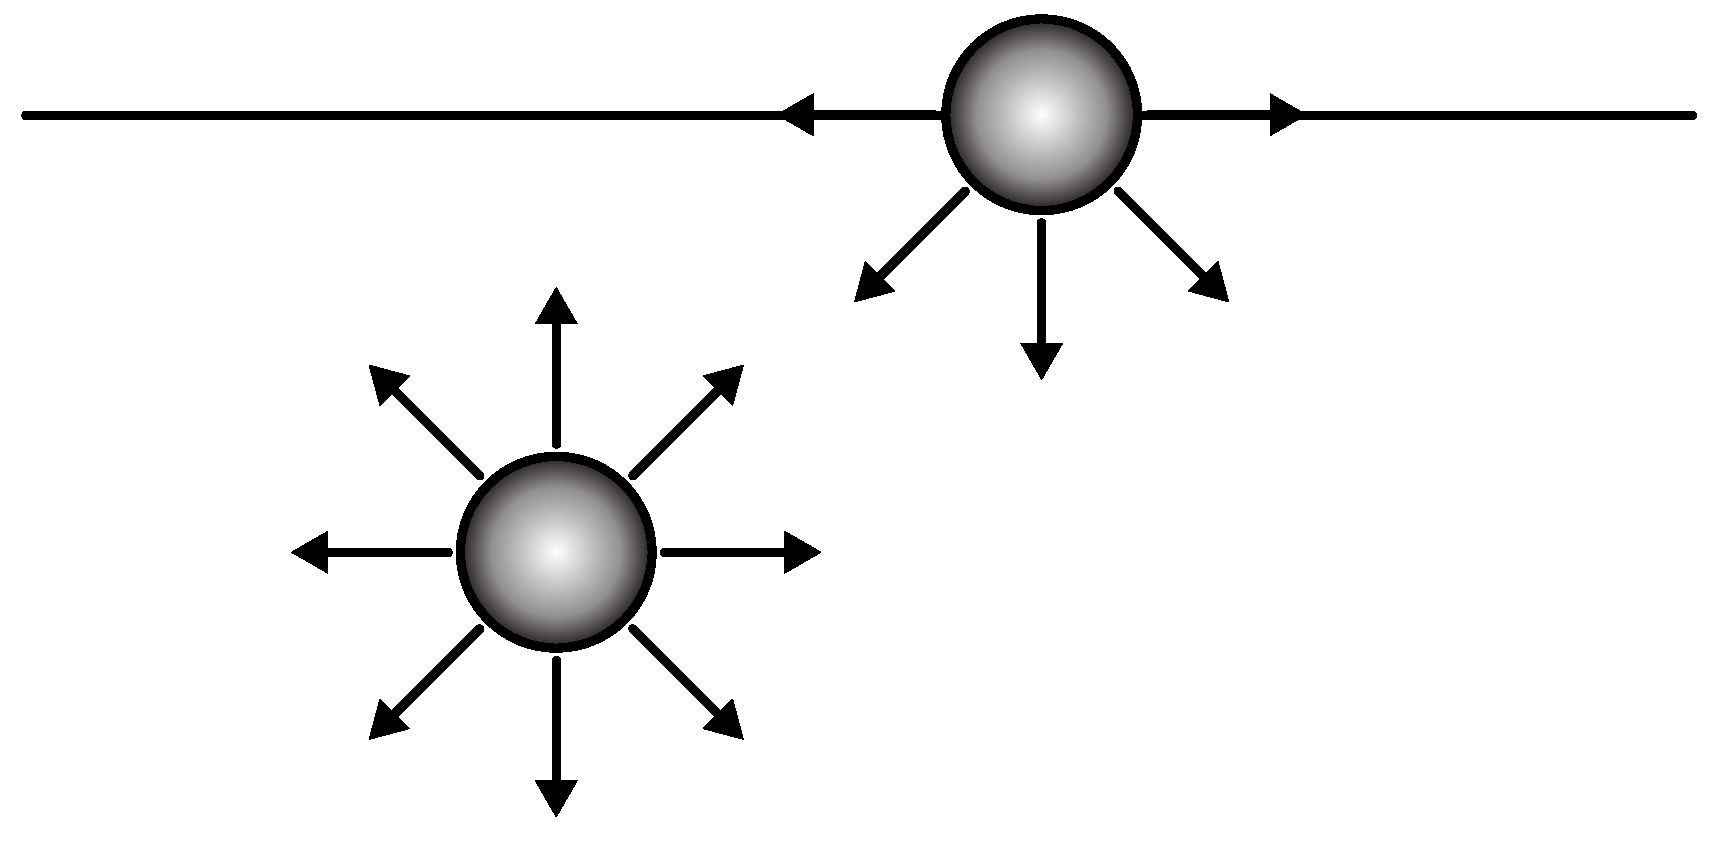
\includegraphics[width=0.7\linewidth]{Chapters/Figures/surface_energy_origin}
	\caption[Surface Free Energy]{A molecule in the bulk has twice as many neighboring molecules than one on the surface, and thus, twice as many neighboring attractions. }
	\label{fig:surfaceenergyorigin}
\end{figure}
The difference in energy per unit area between particles in the bulk compared to the surface is known as the \textbf{surface free energy}, $\gamma$, often written as just surface energy. Equivalently, $\gamma$ can also be defined as the reversible work per unit area to create new surface by cutting. This exposes new particles to the surface. When the surface of a fluid is ``stretched,'' however, new atoms or molecules arrive at the surface, maintaining the number of atoms per unit area as a constant value. Therefore, the surface energy is the same as the surface stress for a fluid and equal to a constant value. Because of this, $\gamma$ and $\Upsilon$ have are often referred to interchangeably as \textbf{surface tension}. While conceptually the energetics are similar in liquid materials, the situation becomes more complicated for materials which cannot flow.


%This difference in energy per unit surface area is known as the surface tension. This setup is true not only for fluids, but also for stiff solids. 
%
%The energy associated with particles in the bulk is less than that of the particles at the surface. Molecules beneath the surface are attracted by the particles around them in every direction. In contrast, the particles at the surface are only attracted by the molecules directly adjacent to them. As a result of these less favorable interactions, they are in a state of higher energy compared to molecules in the bulk. The difference in energy between particles in the bulk compared to the surface is known as the \textbf{surface free energy}, $\gamma$, often written as just surface energy. Equivalently, $\gamma$ can also be defined as the reversible work per unit area to create new surface by cutting. This exposes new particles to the surface. When the surface of a fluid is ``stretched,'' however, new atoms or molecules arrive at the surface, maintaining the number of atoms per unit area as a constant value. Therefore, the surface energy is the same as the surface stress for a fluid and equal to a constant value. Because of this, $\gamma$ and $\Upsilon$ have are often referred to interchangeably as \textbf{surface tension}. While conceptually the energetics are similar in liquid materials, the situation becomes more complicated for materials that cannot flow.

\subsection{Surface Tension in Solids}
In metals, the origin of surface stress, on the atomic scale, derives from the crystalline structure. The epitaxial layer, or surface atoms, reside in a lower electron density and therefore a different equilibrium spacing than the bulk. The bulk atoms force the surface atoms to fit into the epitaxial overlayer of the crystalline substrate. As a result, the surface atoms are strained by the bulk, leaving the surface stressed by the underlying lattice \cite{cammarata1994surface}. 

Theoretical calculations for surface stress generally involve the taking the derivative of the predicted surface free energy with respect to strain. Various methods for metals involve calculating the electronic density, the kinetic energy, and the electrostatic exchange-correlation\footnote{Forgoing the independent electron approximation, the electronic exchange is a measure of deflection due to the presence of other electrons} \cite{GURTIN1978431}. Experimental measurements of surface stress have been around as early as the 1960's, though measurements of strain-dependent surface stress in stiff materials have only been attempted much more recently and returned scant results \cite{mays1968surface,wasserman1970determination,hanneman1962elastic,martinez1990direct,schell1990mechanical}. Metals are an incredibly useful building tool due to their strength\footnote{Strength: the maximum force per unit area a material can withstand}, but their stiffness\footnote{Stiffness: the material's resistance to deformation via strain} also makes measuring properties as a function of strain severely limited, as most metals will fracture after a few percent strain. For most solids, these surface effects go unnoticed in everyday life due to the overpowering effects of the bulk's elasticity compared to any surface energies \cite{miller2000size,dingreville2005surface,duan2005eshelby,sharma2004size,he2008surface,lu2014towards}.



\subsection{Surface Stress Effects in Soft Solids}
For solids of small enough size or soft enough composition, the surface energies can compete with or even dominate the effects of the bulk, resulting in strange and counterinruative material properties. For example, the addition of finite, microscopic, liquid droplets in a soft solid actually stiffens the material \cite{style2015stiffening}. While removing material affects the elastic stiffness, it also increases the surface area. At length scales where surface effects dominate, this increase in surface area has a greater energetic cost, and thus leads to a solid of increased stiffness. Further, surface stresses can drive liquid-like instabilities in soft solids, including rounding out sharp corners \cite{mora2015softening} and solid-cylinder version of the Plateau-Rayleigh instability \cite{mora2010capillarity}.
\todo[inline,color=pink]{Add a sentence or two about adhesion \cite{style2013surface,xu2017direct,Jensen2019SoftMatter,Jensen2017PhysRevX}}

Early observations of $ \Upsilon $ in soft solids came from considering the wetting behavior of liquid droplets on soft solid surfaces \cite{xu2017direct,jerison2011deformation,style2013universal,xu2018surface}. The traditional Young-Dupr\'{e} picture of wetting is shown in Figure \ref{fig:three-phase}.
\begin{figure}[h!]
	\centering
	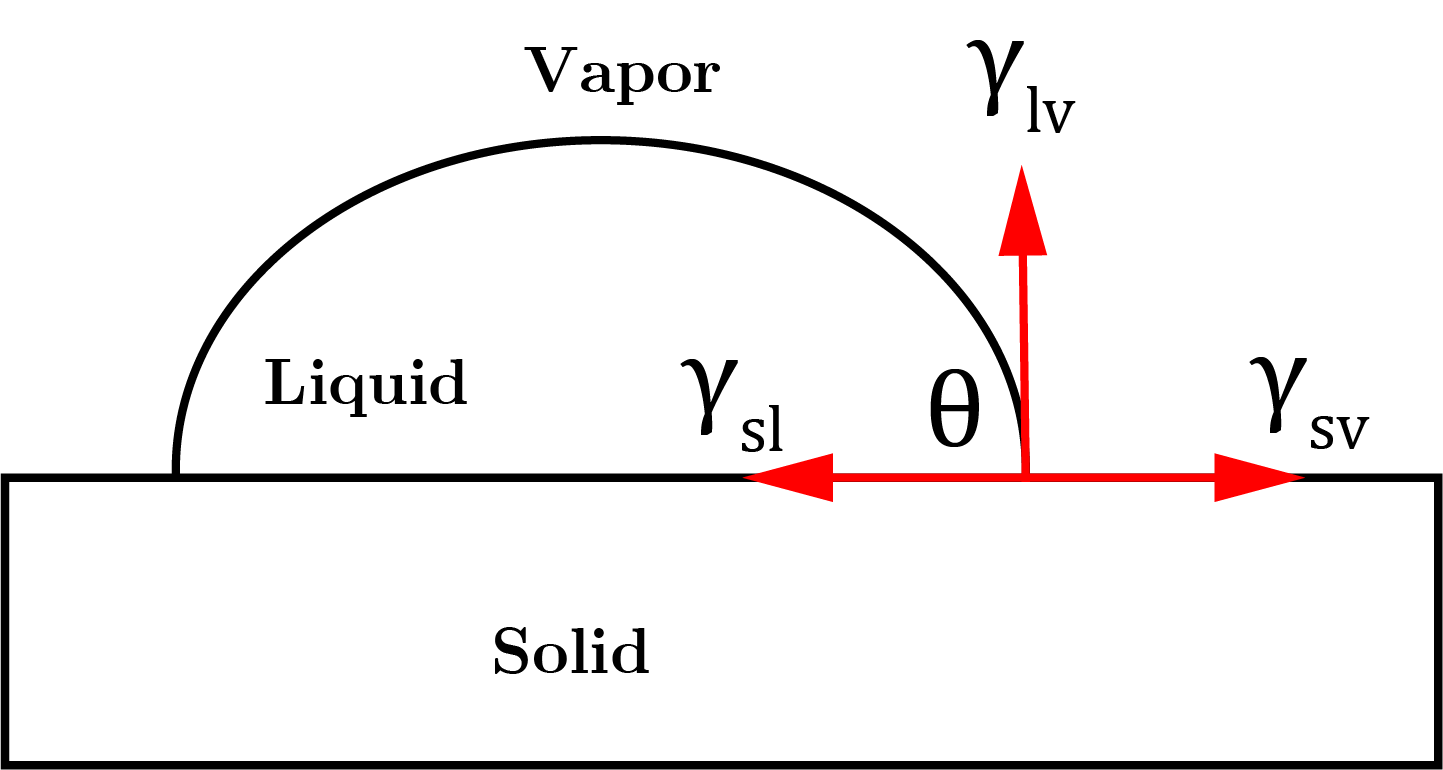
\includegraphics[width=.6\textwidth]{Chapters/Figures/phase_diagram.PNG}
	\caption[Three-Phase Diagram]{Classical Three-Phase Diagram}
	\label{fig:three-phase} 
\end{figure}
This is clearly an unbalanced force diagram in vertical direction; the only vertical force component drawn is the liquid-vapor surface tension, $ \gamma_{lv} $. The normal force from $\gamma_{lv}$ must be balanced by the elastic substrate's resistance to deformation. Calculating this value, however, is still an open question. According to continuum elastic theory, the stress exerted by $\gamma_{lv}$ on the solid diverges at the contact line \cite{jerison2011deformation}. While the field of contact mechanics dates back to the 18th century, seemingly simple problems like a liquid droplet on an elastic surface are still not yet well understood and provide challenging questions when examined on a small enough scale. 

\begin{figure}[h!]
	\centering
	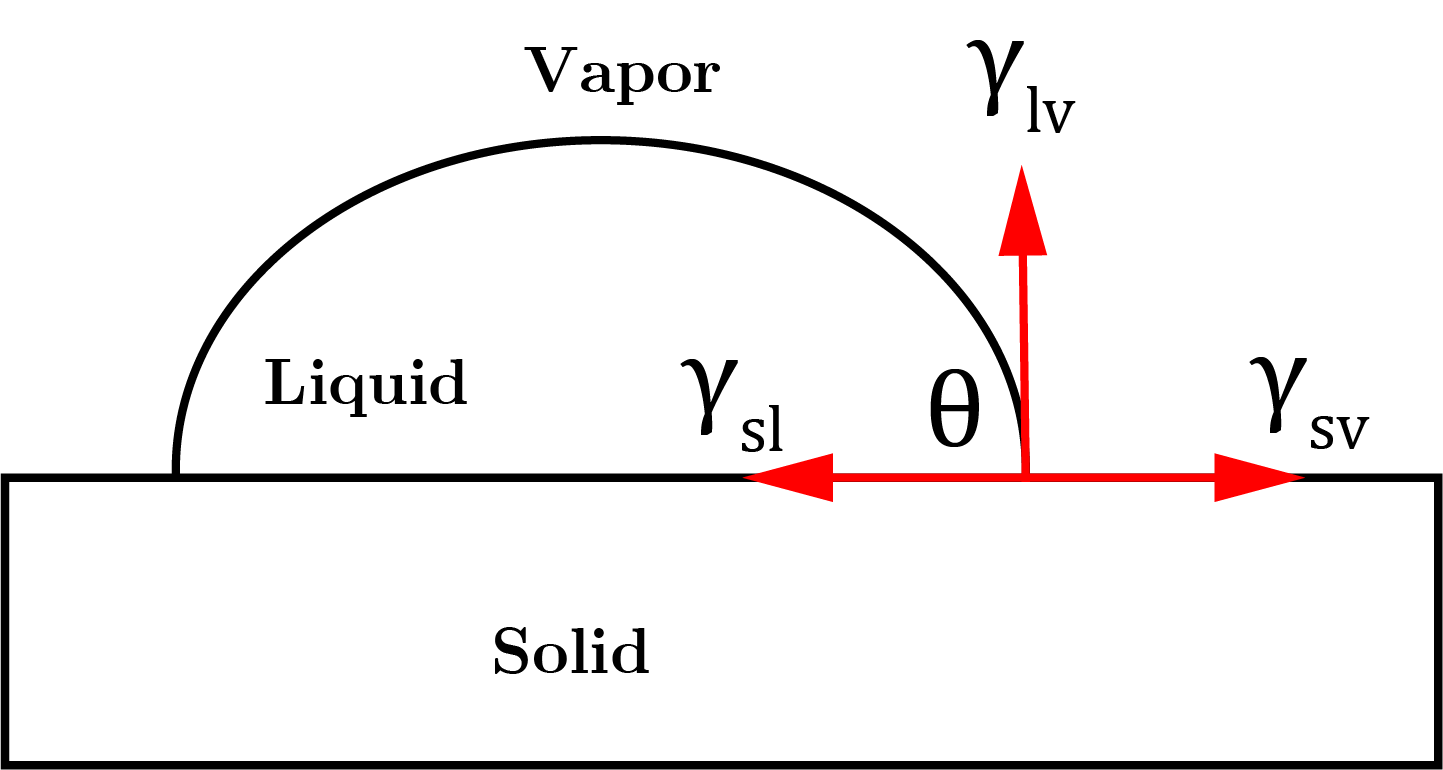
\includegraphics[width=.6\textwidth]{Chapters/Figures/phase_diagram}
	\caption[Three-Phase Diagram: Zoomed]{When inspected on the microscopic scale, the unbalanced three phase diagram of Figure \ref{fig:three-phase} is resolved by the deformation of the substrate. The liquid droplet indents into the solid and pulls the solid up slightly to wrap around itself.}
	\label{fig:three-phase-zoomed} 
\end{figure}

Jerison et al. 2011 \cite{jerison2011deformation} found that modeling the deformation of the elastic substrate due to a liquid droplet fit best by incorporating both the finite thickness and surface tension of the substrate. This new model solved many issues with the previous best solution by Boussinesq: taking into account the finite thickness ensured that the deformations would go to zero far from the contact line, and the substrate's surface tension resolves the single stress singularity, eliminating the divergence of strain and vertical displacement at the contact point \cite{liang2018surface}. This gave us the first method to measure $ \Upsilon $ of a solid directly, tackling a long-standing problem in materials science.
%Note to KEJ: I re-read Jerison 2011. I misread it the first time. In doing their calculations, they assumed the contact angle was close to $ 90\deg $, and they assumed $ \gamma_{sl}=\gamma_{sv} $...but their theory doesn't account for contact angles far from $ 90\deg $....which are the instances in which $ \gamma_{sl}\neq \gamma_{sv} $.


\subsection{Direct Measurement of Solid Surface Stresses}
Measuring the surface stresses even in soft solids has proved experimentally challenging over the years \cite{xu2016surface,jensen2015wetting,mondal2015estimation,style2013surface,jagota2012surface,nadermann2013solid,park2014visualization}. A modern method of measuring the deformation of a soft, elastic solid imposed by the liquid droplet in Figure \ref{fig:three-phase} was introduced by Jerison in 2011 \cite{jerison2011deformation} and later utilized by Style \emph{et al.} in 2013 \cite{style2013universal}. They measured the 3-phase contact line geometry in Figure \ref{fig:three-phase-zoomed} without requiring any prior knowledge about the bulk elastic properties of the substrate material. 

While this technique is effective, it is limited in its applications due to material properties. The method only works for immiscible fluids such that the gel does not absorb the surface droplets. Furthermore, the fluid must also have a low volatility; otherwise, the droplet would begin to evaporate while waiting for the surface deformations to settle. Since then, other methods have been developed, including an adhesion-based technique developed by Style \textit{et al.} in 2013 \cite{style2013surface}. Whereas measurements use the contact angle of liquid droplets, in soft adhesion, the deformation of a soft substrate due to contact with a rigid object depends partially on the surface stress, which can then be extracted using theory (derived in Chapter 2) \cite{tian2018measure,CaoZhen2014EAaW,caoAdhesion}. Though the measurement is less direct, this adhesion based method does not suffer from the same material limitations and give us another approach to measuring $ \Upsilon $.  



%physical crosslinkers: add to ch1 brief descriptions.
%There are two types of crosslinkers: physical and chemical. When physical crosslinkers are stretched, the configuration of the system changes such that the tangled crosslinkers begin to unwind and untangle. From a statistical mechanics perspective, this decreases the configurational entropy, thus increasing the free energy. For chemical crosslinkers, the stiffness is a result of covalent bonds resisting deformation.  

\subsubsection{Puzzling Surface Stress Measurements in Gels}
%In contrast to hard materials, it has been widely assumed that surface stress in soft matter would be nearly strain-independent. 
Surface stress in soft solids is a topic of growing interest. Gels, for example, while classified as solid, are comprised mainly of fluid (by weight) and exhibit many properties that are more closely associated with liquids. Their rigidity is a result a three-dimensional network of crosslinked polymers which entrap large amounts of liquid throughout\footnote{For a more in depth explanation, see section \ref{section:polychem}} via capillary forces. The result is a solid whose stiffness is determined by the composition and temperature.  Unlike in metals, elastocapillary physics plays a crucial role in determining the a soft material's behavioral properties. Furthermore, because the surface stress in liquids is constant and equal to the surface energy of the substance $(\Upsilon = \gamma)$, it was largely assumed that deforming a gel would not have a significant effect on the surface tension, given that the fluid could flow back to the stretched surface of the gel. 

In the following years, further tests of surface stress in soft solids (Table \ref{tab:upsilon_values}) were measured with wildly varying results. It began to become clear that the surface stress of soft solids was not simply that of the fluid phase, and there is more to the mystery. 
\begin{table}[h!]
	\centering
	\begin{tabular}{|l|l|l|l|}
		\hline
		\textbf{Silicone}       & \multicolumn{1}{c|}{\textbf{\begin{tabular}[c]{@{}c@{}}Young's Modulus \\ (kPa)\end{tabular}}} & \multicolumn{1}{c|}{\textbf{\begin{tabular}[c]{@{}c@{}}Measured $\Upsilon$ \\ (mN m$^{-1}$)\end{tabular}}} & \textbf{Reference} \\ \hline
		Sylgard 184             & 770                                                                       & 19                                & \cite{xu2016surface}                                                                       \\ \hline
		Gelest                  & 5.6                                                                       & 20                                                                                    &                    \cite{jensen2015wetting}\\ \hline
		Sylgard 184             & 2400                                                                      & 26                                                                                 &                 \cite{mondal2015estimation}   \\ \hline
			Dow Corning CY52-276A/B & 3                                                                         & 30                                                                                    &                 \cite{style2013universal}   \\ \hline
		Sylgard 184             & 18                                                                        & 30-70                                                                                 &                  \cite{jagota2012surface}\\ \hline
		Sylgard 184             & 1000                                                                      & 40-50                                                                                 &                 \cite{nadermann2013solid}   \\ \hline
		
	
		Dow Corning CY52-276A/B & 3                                                                         & 42-59                                                                                 &                  \cite{park2014visualization}  \\ \hline
	\end{tabular}
	\caption[Measured $\Upsilon$ Values]{A Collection of Previously Measured $\Upsilon$ Values}
	\label{tab:upsilon_values} 
\end{table}
The mystery of measure $ \Upsilon $ discrepancy would be solved if $ \Upsilon $ was not constant, but, instead, dependent on the deformation state of the material. The idea that $ \Upsilon $ may be strain dependent ($ \Upsilon(\epsilon) $) goes back to the classical theory of $ \Upsilon $ in metals, but had never been full experimentally verified. 

\subsubsection{Strain Dependence of Surface Stress in Traditional Solids}
Although surface tension is most familiar in liquids, it is a property shared by solids as well.  In contrast to liquids, when a surface of a solid is elastically stretched, the number of atoms per unit area changes, such that generally $ \gamma \neq \Upsilon$ in solids \cite{cammarata1994surface}. The relationship between surface energy and surface stress can be derived through the use of the elastic deformation tensor $\epsilon_{ij}$, where $i,j=1,2$. We can then define $d\epsilon_{ij}$ to be an infinitesimal and elastic (reversible) strain as a result in a variation of the surface area, $A$. The surface stress tensor, $\Upsilon_{ij}$, is the work associated with the variation in the excess free energy of the surface due to strain, $\gamma A$. Thus, we can write, \[d(\gamma A) = A \Upsilon_{ij} d\epsilon_{ij}\] Expanding out the first term, $d(\gamma A) = \gamma dA + A d\gamma$. Utilizing symmetries, we can say that $dA = A \delta_{ij} d\epsilon_{ij}$, where $\delta_{ij}$ is the Kronecker delta. Making the substitution, we find \[\gamma dA + A d\gamma = \gamma A \delta_{ij} d\epsilon_{ij} + A d\gamma = A \Upsilon_{ij} d\epsilon_{ij}\] And thus,
\begin{equation}
\label{shuttleworth_eqn}
\Upsilon_{ij} = \delta_{ij}\gamma + \frac{\partial \gamma}{\partial \epsilon_{ij}} 
\end{equation}
This (\ref{shuttleworth_eqn}) is known as the Shuttleworth Equation, and clearly shows that both $\gamma$ and $\Upsilon$ in solids should be dependent on the strain state of the material.

Soft solids provide a unique opportunity to measure strain-dependent surface stress. Despite being a solid, soft solids, such as gels, can easily be stretched elastically. In 2017 Xu, Jensen et. al \cite{xu2017direct} made the first direct measurement of strain-dependent surface stress in solids. Their measurements suggest a surprisingly strong linear relationship between surface-stress and strain, measuring that the surface stress of their PDMS substrate more than doubled at 20\% strain. Additionally, their method of measurement is limited to a select combination of materials. 

We have developed a method for measuring strain dependent surface stress that is applicable to a wide variety of soft, compliant materials. We have measured $ \Upsilon $ and $ W $ in two varieties of PDMS using this soft adhesion approach. However, our attempts to measure these values as a function of strain have been met with an unexpected amount of noise.   In this thesis, I present the full background, methods, and underlying physics of the process, as well as the $ \Upsilon $ and $ W $ measurements and preliminary $ \Upsilon(\epsilon) $ and $ W(\epsilon) $ work.  
%To measure the surface stress of the material, the group utilized Jerison's 2011 method \cite{jerison2011deformation}. First, a glycerol or flurinaeted oil droplet is placed atop a soft, elastic silicone gel substrate. To measure surface deformations, the substrate is first coated with fluorescent beads, which can subsequently be measured using confocal microscopy. The located positions of the fluorescent beads outline the surface and allows for reconstruction of the surface deformations.

%Balancing, we find
%\[F_{vertical} = \gamma * \sin(\theta) = E * \delta,\]
%where $F_{vertical}$ is the force per unit length in the vertical direction, $\gamma$ is the surface tension of the liquid, E is the Young's modulus of a substrate, and $\delta$ is deformation of the substrate. Zooming


 



%\subsubsection{Surface Tension and Contact with Soft Elastic Solids}
%Over the last few years, there has been a significant amount of work regarding adhesion in soft solids. We want to take advantage of what is known about the role of surface stress in the contact mechanics of soft solids to directly measure the surface stress while varying the properties of the underlying substrate. In doing so, we will have created a new form of measuring strain-dependent surface stress, applicable to a broad array of stretchable materials. The contact angle based method used in the first direct measurement of $ \Upsilon(\epsilon) $ \cite{xu2017direct} is limited to a select combination of materials, as the liquid droplet must be immiscible and non-volatile. We hope to apply Style's 2013 technique to stretchable substrates in order to measure $ \Upsilon(\epsilon) $ for a wider variety of materials. The specifics of this technique are covered in the following chapter.

\section{Outline of the Thesis}
This thesis begins with a derivation of modern theory of contact mechanics for soft solids. With this in mind, we proceed to outline the experimental design and setup in chapter 2, followed with an example of data aquisition and image analysis in chapter 3. Chapter 4 contains our preliminary surface stress and adhesion results for various materials. Finally, chapter 5 looks ahead, discussing possibilities for future experiments and improvements to the experimental process.

\chapter{Experimental Approach: Setup, Data Acquisition, \& Analysis }
In this chapter we discuss the setup of the experiment from start to finish. First we discuss the underlying theory required for the technique. Next, we walk through the walk through the experimental setup, the process of acquiring data and processing it for a single sphere. Finally we address the stretching apparatus, including its calibration process, and analyzing the results. Further details can be found in the appendices.

\section{Measuring Surface Stress via Adhesion}
\subsection{Beyond Hertzian Mechanics and JKR Theory}

Hertzian Mechanics, developed by Heinrich Hertz in the 1800's, allows for the calculation of stress and deformation based on the elastic moduli of the contacted surfaces, as well as their radii of curvature and applied force. While Hertzian mechanics stood for a long time, it neglected to take into account the adhesion energy of the system.  

In 1971, Johnson, Kendall, and Roberts (JKR) sought to remedy this omission by developing a classical theory of contact mechanics that balances the forces of adhesion with elasticity from the bulk and the surface free energy {\cite{johnson1971surface}}. Today, it is still the standard theory used to interpret and soft contact situation. However, it has recently been shown that while JKR theory is a great improvement over Hertztian Mechanics, it breaks down in the elastocapillary regime.\todo[color=pink]{add citation} Specifically, at lengths where 
\begin{equation}
\label{EC_regime}
L_{c} \leq \frac{\Upsilon}{E}
\end{equation}
the surface energies compete with those of the bulk and can no longer be ignored. Fittingly, $L_c$ is referred to as the elastocapillary length. By understanding the role of surface tension in soft adhesion, we can measure the physical properties of a balanced system in the elastocapillary regime and hence measure the surface stress and adhesion energy from the balance of forces.



\subsection{Force Balance Derivation}
When materials are soft or small enough, three main forces balance to determine the contact mechanics of the system. Consider a marble sinking into a soft, sticky substrate. Adhesive forces increase the contact area between the marble and the substrate. Increasing the contact area has the effect of ``pulling'' the marble into the gel. As a consequence, the substrate is being compressed [vertically], which is counteracted by the elastic forces within the bulk. This compression also has the effect of stretching the surface of the substrate, which is counteracted by substrate's surface tension. Below, we calculate the energy term associated with each of the forces acting on a dense sphere sinking into a soft substrate. Note, for such a small sphere, the force of gravity is negligible and need not be taken into consideration. For example, a silica (silicon-dioxide) microsphere has a density is $2.65$ g/cm$^3$. For a very large sphere with radius 50 microns, gravity only applies a force of roughly 1.02e-08 N.

\subsubsection{Elastic Energy}
The energy required to make a circular indentation of radius R and depth d can be derived from Hertzian contact mechanics \cite{hertz1882uber, style2013surface,cao2016nanoparticles}. Contact between a sphere and an elastic half space\footnote{i.e. the contact area is $ \ll $ the characteristic radius of the object. A flat plan can be thought of as $ R = \infty $}   is a classic Hertzian contact problem. It is easiest to calculate the force and then integrate to determine the potential energy. For two elastic surfaces in contact with no externally applied forces, the force from elastic contact is:

\begin{equation}
F = \frac{4}{3}E^*R^{1/2}d^{3/2}
\label{elastic_force_eqn}
\end{equation} 
where 
\begin{align*}
\frac{1}{E^*} = \frac{1-\nu_{sphere}^2}{E_{sphere}} + \frac{1-\nu_{substrate}^2}{E_{substrate}} 
\end{align*}
For a glass sphere sinking into a soft substrate, $ E_{sphere} \gg 1-\nu_{sphere}^2 $, so this first term can be dropped as a reasonable approximation\footnote{$\nu_{Si0_2} \approx .17 $ and $ E_{Si0_2} \approx 70 \cross 10^9 $ Pa}. Thus we can approximate $ E^* \approx \frac{E_{substrate}}{1-\nu_{substrate}^2} $. Substituting this into equation (\ref{elastic_force_eqn}), we find:

\begin{equation}
F \approx \frac{4}{3}\frac{ER^{1/2}d^{3/2}}{1-\nu^2}
\label{elastic_force_eqn2}
\end{equation}
Because $F = \frac{\partial U}{\partial d}$, we can simply integrate equation (\ref{elastic_force_eqn2}) to obtain the energy relation:
\begin{equation}
\label{elastic_energy}
U_{elastic} \approx  \frac{ER^{1/2}d^{5/2}}{1-\nu^2}
\end{equation}


\subsubsection{Adhesion Energy}
The energy of adhesion is W multiplied by the surface area in contact (as found above). Namely,
\begin{equation}
\label{W_energy}
U_{adhesion} \approx -2\pi W R d 
\end{equation}
where W is the adhesion energy. \todo[inline,color=pink]{I think I should explain adhesion somewhere and talk about the Dupre equation 1869. Not sure where I want to put this, however.}. 

\subsubsection{Surface Energy}
$\Upsilon$ is the surface stress, which is equal to the energy cost per unit area required to create surface via cutting or stretching the material. For a flat substrate being stretched via the indendation of a sphere, the energetic cost is
\begin{equation}
\label{generic_surface_energy}
U_{surface} = \pi \Upsilon_{sv}\Delta A
\end{equation}
where $\Delta A$ is the change in surface area when stretched by part of an indenting sphere (spherical cap). Determining the change in area is a simple geometrical problem.

\begin{equation}
\Delta A = A_{cap} - A_{circle}. 
\end{equation}
Let $ a $ be the base radius of the circle projected on the plane of the substrate's surface. Let R be the radius of the indenting sphere, and d be the depth into which it is stretching. We can find a relationship between these variables using the Pythagorean theorem.

\begin{SCfigure}[][h]
	\begin{minipage}{.5\textwidth}
	\begin{align*}
	&a^2 + (R-d)^2 = R^2 \\
	&a^2 + R^2 - 2Rd +d^2 = R^2 \\
	&a^2 = 2Rd -d^2 \\
	&a^2 + d^2 = 2Rd
	\end{align*}
	\end{minipage}%
	\begin{minipage}{.5\textwidth}
	\centering
	\caption{Spherical Cap Geometry}
	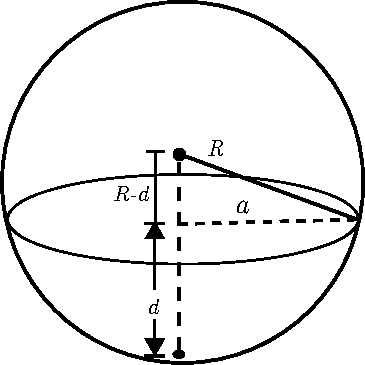
\includegraphics[width=.5\linewidth]{Chapters/Figures/SphericalCap}
	\label{fig:sphericalcap}
	\end{minipage}
\end{SCfigure}
Now, solving for $ \Delta A $ and using the above relationship in the last step, we find:
\begin{align*}
\Delta A &= 2\pi Rd - \pi a^2 \\
&= \pi(a^2+d^2) - \pi a^2 \\
&= \pi d^2
\end{align*}
 Rewriting (\ref{generic_surface_energy}), we can simplify surface energy in this geometry as 
 
 \begin{equation}
 \label{surface_energy}
 U_{surface} = \pi \Upsilon_{sv} d^2
 \end{equation}

\subsubsection{Force Balance}
At static equilibrium, the sum of the energies is:
\[U_{total} = \Upsilon_{sv} \pi d^2 + \frac{cER^{1/2}d^{5/2}}{1-\nu^2} - 2\pi W R d\] 
where c is a geometric factor to be determined in the next step. We can re-arrange the equation such that the sum of forces is equal to zero and differentiate both sides with respect to depth.

\begin{equation*}
\frac{\partial U_{total}}{\partial d} = \Sigma F = 0
\end{equation*}
\begin{equation}
\label{THEeqn}
2 \pi \Upsilon_{sv}d  + \frac{5cER^{1/2}d^{3/2}}{2 \left( 1-\nu ^2 \right) }  - 2 \pi WR = 0
\end{equation}

Where $ c = \frac{8}{5\sqrt{3}} $. This value of c is chosen to recover classical JKR theory, which predicts an indentation of $ d =  \left[\frac{\sqrt{3}\pi W (1 - \mu^2)}{2E} \right]^{2/3}R^{1/3}$ \cite{style2013surface, johnson1971surface}. This energy balance was first published in 2013 by Styles et al. in \textit{Nature Communications} \cite{style2013surface}. \todo[inline, color=pink]{KEJ: Why did you want me to mention Jensen PNAS 2015? Wasn't this the phase separation paper? What connection were you thinking I should make here?}


\subsection{Experimental Approach}
Equation \ref{THEeqn} gives us a quantitative relationship between the spontaneous indentation depth, $ d $, sphere radius, $ R $, and key material properties: $ \Upsilon, E, \nu, \text{and }W $. The Young Modulus, E, and the Poisson ratio, $\nu$ of the substrate can be measured separately for the substrate material. The depth $d$, and the radius $R$ of the sphere can be measured using fluorescent confocal microscopy, as described in section \ref{ch:microscopy}. The only remaining terms, $W$ and $\Upsilon$, the adhesion energy and the surface stress, respectively, can be determined with a two-parameter fit of $ d $ vs. $ R. $

\section{Preparing a Substrate}
In the following section, we outline the process of preparing a soft substrate for testing. The process is similar for a zero strain sample and a stretchable sample, and we make clear any distinctions between the two processes. Specific details for our substrate types can be found in Chapter 4.

Before preparing the substrate, we prepare the surface on which the substrate will be held, from hereon referred to as the underlayer. For a non stretched sample, we use a glass coverslip, and for a stretched sample we use a thin PDMS sheet. \todo[color=pink]{I don't like underlayer name. Base plate? Substratum base?} We first coat this layer with fluorescent beads in order to later locate the bottom of our substrate. In preparing our substrate, there are two important factors to consider: thickness and evenness of the surface. The substrate must be thick enough such that the the indenting spheres do not feel a measurable force from the glass or PDMS underlayer. This bottom layer of fluorescent beads allows us to easily gauge the thickness of our substrate. It is important that our substrate has an even surface, otherwise it is difficult to determine the sphere's depth, $ d $. To achieve this, we use a technique called spin-coating where we place our uncured substrate (when it still has liquid like viscosity) on the underlayer and spin it rapidly for a period of time. The angular momentum causes the flings the fluid away from the center of the underlayer. The result of this process is an even coating which will cure into our substrate over the next day.

Once cured, we deposit a second layer of fluorescent beads on the surface. These act as tracer particles which outline the indentation sphere. Using fluorescent confocal microscopy, we are able to precisely locate each fluorescent bead and outline the indentation sphere. It is important that the beads are dense enough to give a high resolution, yet not so dense as to become indistinguishable; this presents a challenge the MATLAB particle locating software. For a stretchable sample, we place the substrate, now cured onto the stretchable PDMS underlayer, onto the lubricated stretching apparatus. It is important remove any small bubbles on the stretcher's ring to ensure an airtight seal. 

The final preparation step is to sprinkle silica spheres of a range in size on top of the silicone. This should be done at least 30 minutes before collecting data so that the spheres have time to settle into an equilibrium state into the silicone. From a side view, the final setup should look like Figure \ref{fig:substrategraphic}.
\begin{figure}[h!]
	\centering
	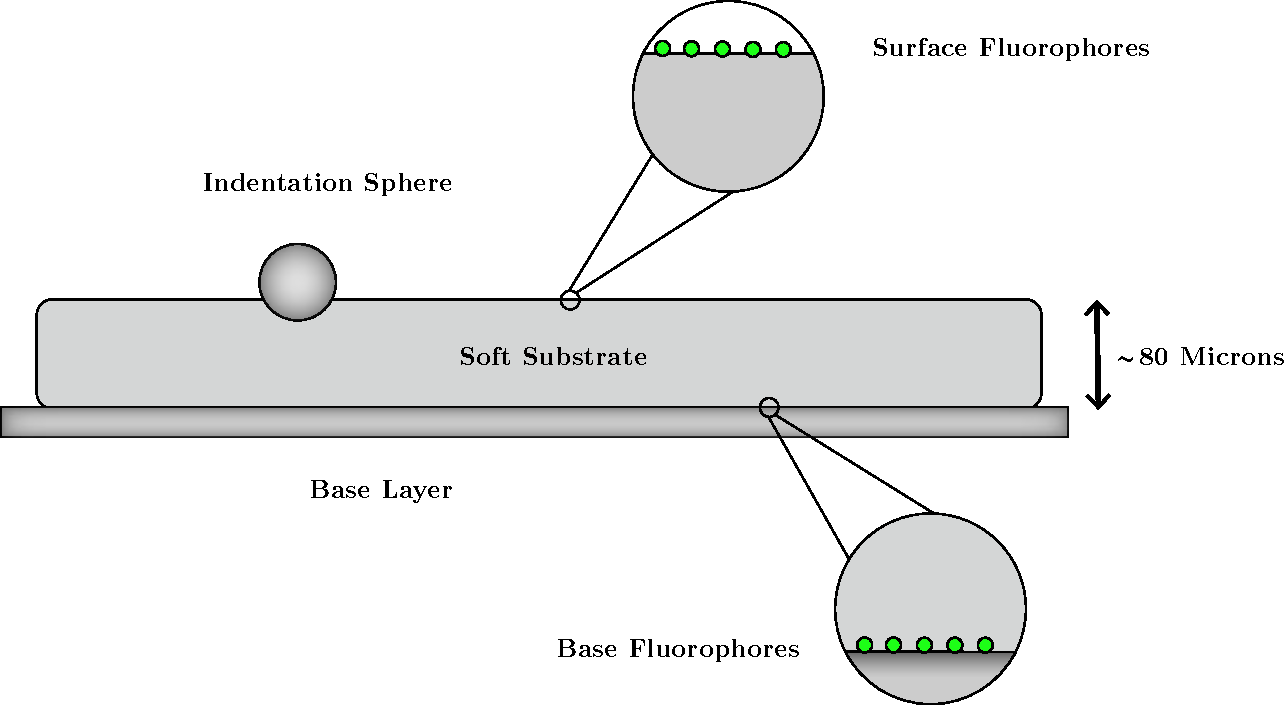
\includegraphics[width=\linewidth]{Chapters/Figures/substrate_graphic_new}
	\caption[Prepared Substrate Profile]{Above is the side profile of a prepared substrate sample. There are two layers of fluorescent beads: the bottom layer is used to measure the substrate's thickness, and the surface layer is used to outline the profile of the larger, indenting sphere. The soft substrate sits on an underlayer, namely glass or a stretchable PDMS silicone.}
	\label{fig:substrategraphic}
\end{figure}


\section{Stretching Apparatus}
Our interest is not just in  measuring, $W$ and $\Upsilon$ for a given substrate, but in understanding how those values change when under strange As needed, we have built our own equibiaxial stretching apparatus capable of maintaining up to 35\% strain in our silicone samples. The design is based off of previous work designed for stretching biological tissues \cite{na2008time} and is similar in design to the apparatus used in the 2017 $\Upsilon(\epsilon)$ measurements \cite{xu2017direct}. Below is a general description of the design, though detailed design documents can be found in Appendix A.

\subsection{Stretcher Design}
Geometrically, the stretching apparatus is constructed of two concentric cylinders connected at the base to create a channel between them. The top of each ring is flat, apart from a slight chamfer to reduce the risk of ripping the sheet as it is stretched. Each ring is then coated in Dow Corning vacuum grease to make a seal. It is critical that the inner ring has an ample amount of grease so that when a vacuum is pulled in the channel, the sheet will stretch from the center outwards  and not from the edges inwards. The sheet is held in place with an o-ring wrapped around the outside of the cylinder, which is then clamped down by a removable outer ring using a tension clamp. The tension provided by the o-ring and clamp ensure that a solid vacuum is kept and the edges of the sheet are minimally stretched into the trough.add to appendix?  

\begin{figure}[h!]
	\centering
	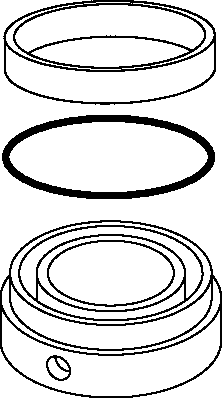
\includegraphics[width=.5\linewidth]{Chapters/Figures/exploded_stretcher}
	\caption[Stretching Apparatus Design]{Here is an exploded view of the stretching apparatus. The substrate goes on top of the base (substrate side down). It is then held down with an o-ring, which sits on the outside ledge. A second ring sits on top of the o-ring and is then held down by the microscope mount (not pictured here).}
	\label{fig:explodedstretcher}
\end{figure}
\begin{figure}
	\centering
	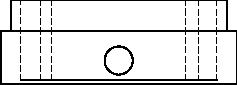
\includegraphics[width=0.7\linewidth]{Chapters/Figures/stretcher_side}
	\caption[Side Profile of Stretching Apparatus]{Above is the side profile of the stretching apparatus. Note the channel attached at the base, and the large center hole at the base where our substrate can be accessed by the microscope.}
	\label{fig:stretcherside}
\end{figure}


A tapped screw hole on the side of the apparatus connects the chamber to a syringe via thin, plastic tubing. To pull a vacuum in the channel, we withdraw air using a syringe pump. This allows us to have a consistent withdraw rate and control over the amount of air withdrawn to a high degree of precision.

\section{Calibration}
Originally, we intended to calibrate the strain value induced by the vacuum to the extent that we could predict the induced strain based on the amount of air withdrawn from the stretching apparatus. We withdrew air from the syringe and measured the movement of glass spheres adhered to the surface using a 10x air lens on our Nikon confocal microscope. Using the transmission detector allowed us to image the surface of our material with a wide field of view. Strain percentage was calculated using MATLAB code \cite{xu2017direct} \todo[color=pink]{Better/more citations for strain code?}.

There are several obstacles in calibrating the induced strain. First, the stretching apparatus works best when a large strain is applied. Applying small strains one after another works but there is a threshold to induce stretch. No stretching change is visible if less than 2ml is withdrawn from the cylinder per increment. Thus, there is a limited resolution to our calibration data, which would not be a problem if the strain was linear. However, preliminary measurements indicated that the applied strain was nonlinear. This agrees with the with previous results \cite{na2008time} obtained using a similar device. \emph{note to self, double check this is where that graph I'm thinking about actually showed up}. Lastly, the greatest problem with calibrating strain is that we change substrates often. Even if we were to use the same exact sample, by removing it and setting up the device again, there is no way to standardize a zero-applied strain point. To prepare the stretching device, the sample is placed over the opening and a rubber o-ring is placed around the sample to help affix it in place. The sample must then be stretched and wiggled around slightly to remove any snags that could jeopardize the vacuum's efficacy. This means that every time a new sample is prepared, it is in an unknown and unique state of induced strain. It could even have less than zero strain if the sample is loose in large center opening \emph{Think of better name for this.} 

It was thus determined best to measure strain every time we applied a new strain to the silicone substrate and compare it to the substrate's original state. This also assured us that we knew the correct strain value to a higher precision for any given data set. Additionally, with the pleasantly unexpected ability to hold strains exceeding 30\%, the $2\mu$m resolution  limit became superfluous in seeking to measure $\Upsilon(\epsilon)$.


\subsection{Measuring Strain}
To determine the induced strain, we maximized the field of view. This allows us to see how more spheres are shifting, and thus gives a more accurate estimate of induced strain. As such, we decided to switch to the bright-field and measure how the spheres were shifting when stretched. We used a 10x air lens in conjunction with the transmission detector on our Nikon Confocal. We adjust the settings to give decent contrast, but it is more important to have the spheres in focus. For our Nikon this usually means setting the Power (HV) to 80. Each sphere reflects light, and it is this reflection that our particle locating software tracks after some image processing. An example image is located below (Fig.\ref{fig:TDpreandpost}), next to the same image after adjusting the contrast to help our tracking software with particle locating: 

\begin{figure}[h!]
	\begin{tabular}{cc}
		
\includegraphics[width= .48\linewidth]{Chapters/Figures/1xzoom_constellation_zeroStrain.png} & 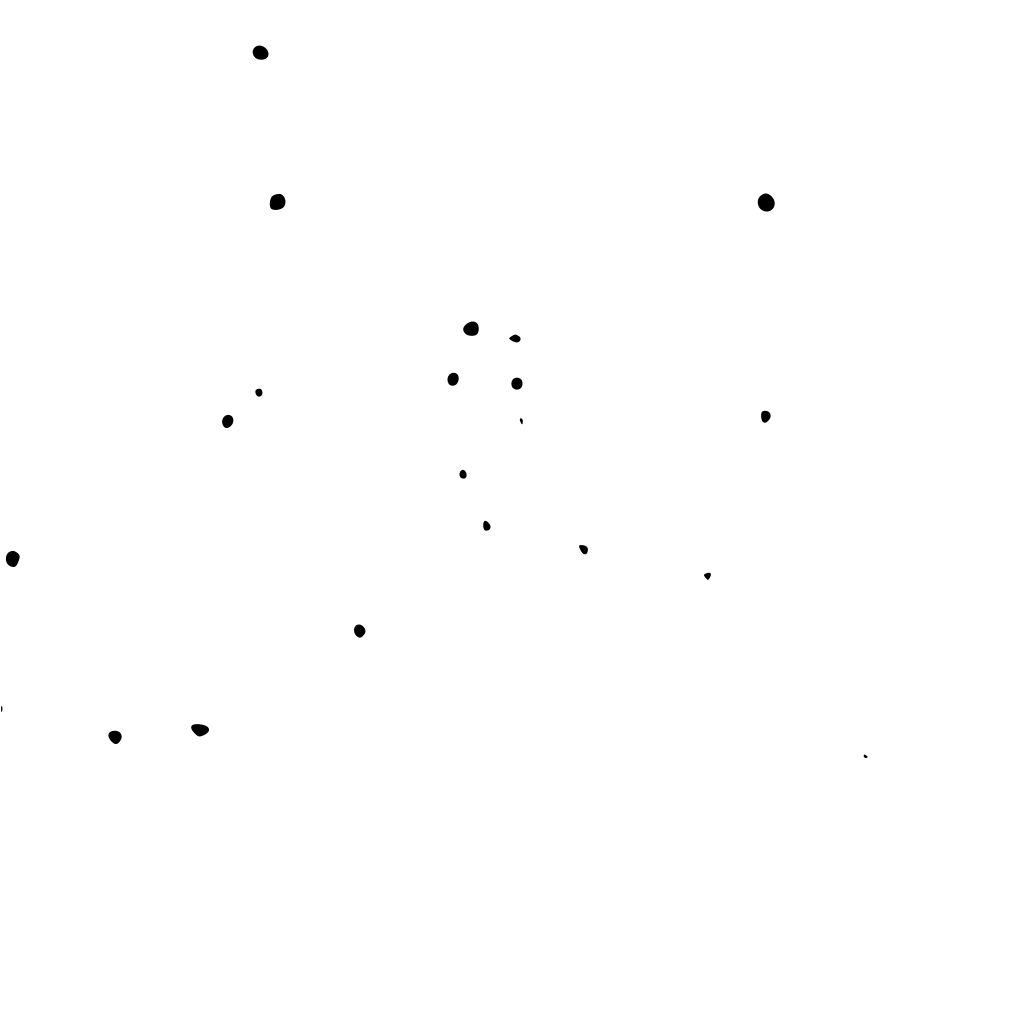
\includegraphics[width= .48\linewidth]{Chapters/Figures/1xzoom_constellation_zeroStrain_supercontrast.png}\\
		Fig. A & Fig. B
	\end{tabular}
	\caption[Bright-field pre and post image processing]{Figure A shows the calibration constellation before any strain is applied. Fig. B shows the same image after processing. Only the sphere reflections remain.}
		\label{fig:TDpreandpost}
\end{figure}

To track how the substrate stretches, we first find a centrally located group of spheres, or ``constellation.'' A good constellation is one that easily identifiable for relocation and tracking purposes, and one that has many discrete points in the field of view - i.e. there are plenty of non-overlapping spheres. \emph{It is an added bonus to find 4 spheres perpendicularly located, such that they form the tips of cross.} Though not necessarily, this is useful for a preliminary strain calculation using the built in measuring functions on the Microscope's software. It is nice to track the progression of stretching and ensure the substrate is not preferentially stretching in on direction; this could indicate the substrate is caught in the apparatus. Not only does this ruin the symmetry assumptions being made for our calculation, but it could lead to the substrate tearing if more strain is being applied than expected.

To evacuate the cylinder, we use the the Harvard Apparatus\texttrademark \ Elite Pro Syringe Pump with a 50ml Luerlock syringe. Before beginning any stretching, we withdraw a few ml of air to ensure the substrate is flat and not sagging. At this point we take a picture of the brightfield and call it the ``zero applied strain'' image. We compare all stretched data to this image in order to determine the induced strain. Because of the geometry of the stretching apparatus, along with the way the silicone cures, it is difficult \emph{impossible??} to determine the true strain of the silicone. However, we are most interested in the slope of the $\Upsilon$ vs. $\epsilon$ curve, $\Lambda$, so this is not vitally important.

The induced strain is a tensor of rank two. Because we are stretching the substrate equally in all directions, we can just look at the magnitude of the tensor and treat the strain as a scalar.     


\begin{figure}[h!]
	\centering
	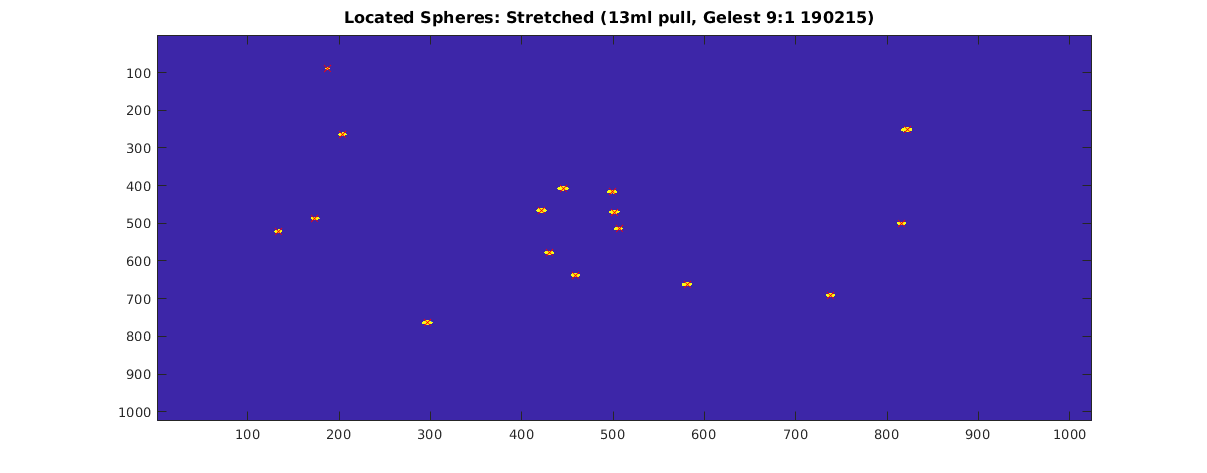
\includegraphics[width=\linewidth]{Chapters/Figures/13ml_stretched_2D_located}
	\caption[Unstretched]{}
	\label{fig:13mlstretched2dlocated}
\end{figure}

\begin{figure}[h!]
	\centering
	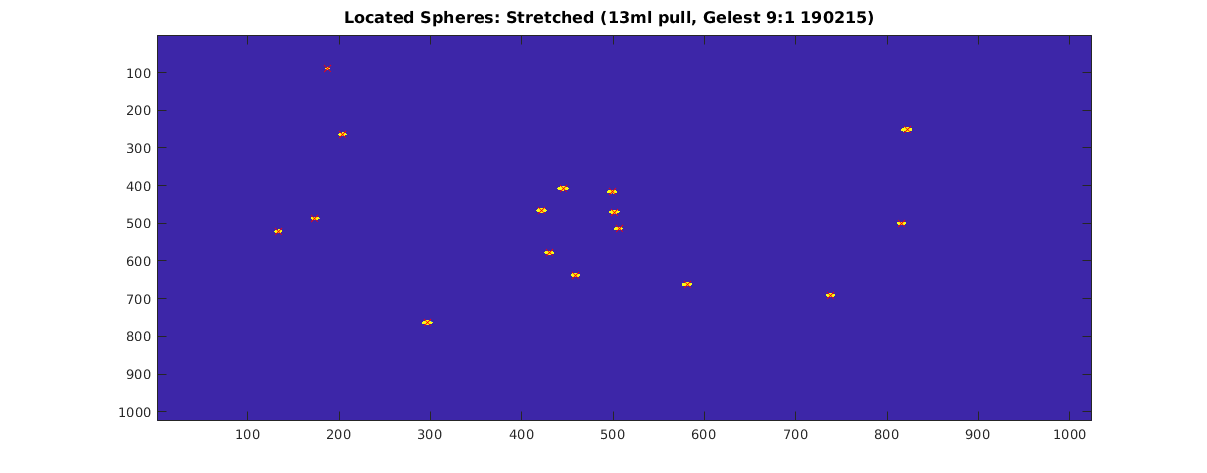
\includegraphics[width=\linewidth]{Chapters/Figures/13ml_stretched_2D_located}
	\caption[Stretched]{These are placeholders for now. I don't really like how they look and I don't think they're totally necessary. It might be nice to keep them if I can clean them up. Especially if I get some nice stretch data with the new DC}
	\label{fig:13mlstretched2dlocated}
\end{figure}
\todo[inline,color=pink]{There's an alternate image where each point is an x for before after. Replace figure with that and zoom in on sphere cluster.}

\section{Material Characterization}
To measure the stiffness of our substrate, we do not use the confocal measurement sample. Instead, when preparing the sample, we cure a surplus of the substrate material in a vial to test the bulk characteristics of the sample. 

We take a standard bulk stiffness measurement using the \todo[color=pink]{Include Brand Name}texture analyzer. A rigid cylinder with radius $R = 1.5$ mm is slowly indented into the bulk substrate. The force response vs. indentation depth is recorded for several tests with varying starting heights and locations (See Figure \ref{fig:Bulkstiffness_raw}). We use the average E value obtained from these tests in our W,$ \Upsilon $ fitting. The fitting processed will be reviewed in Chapter 3. 
\begin{figure}[h!]
	\centering
	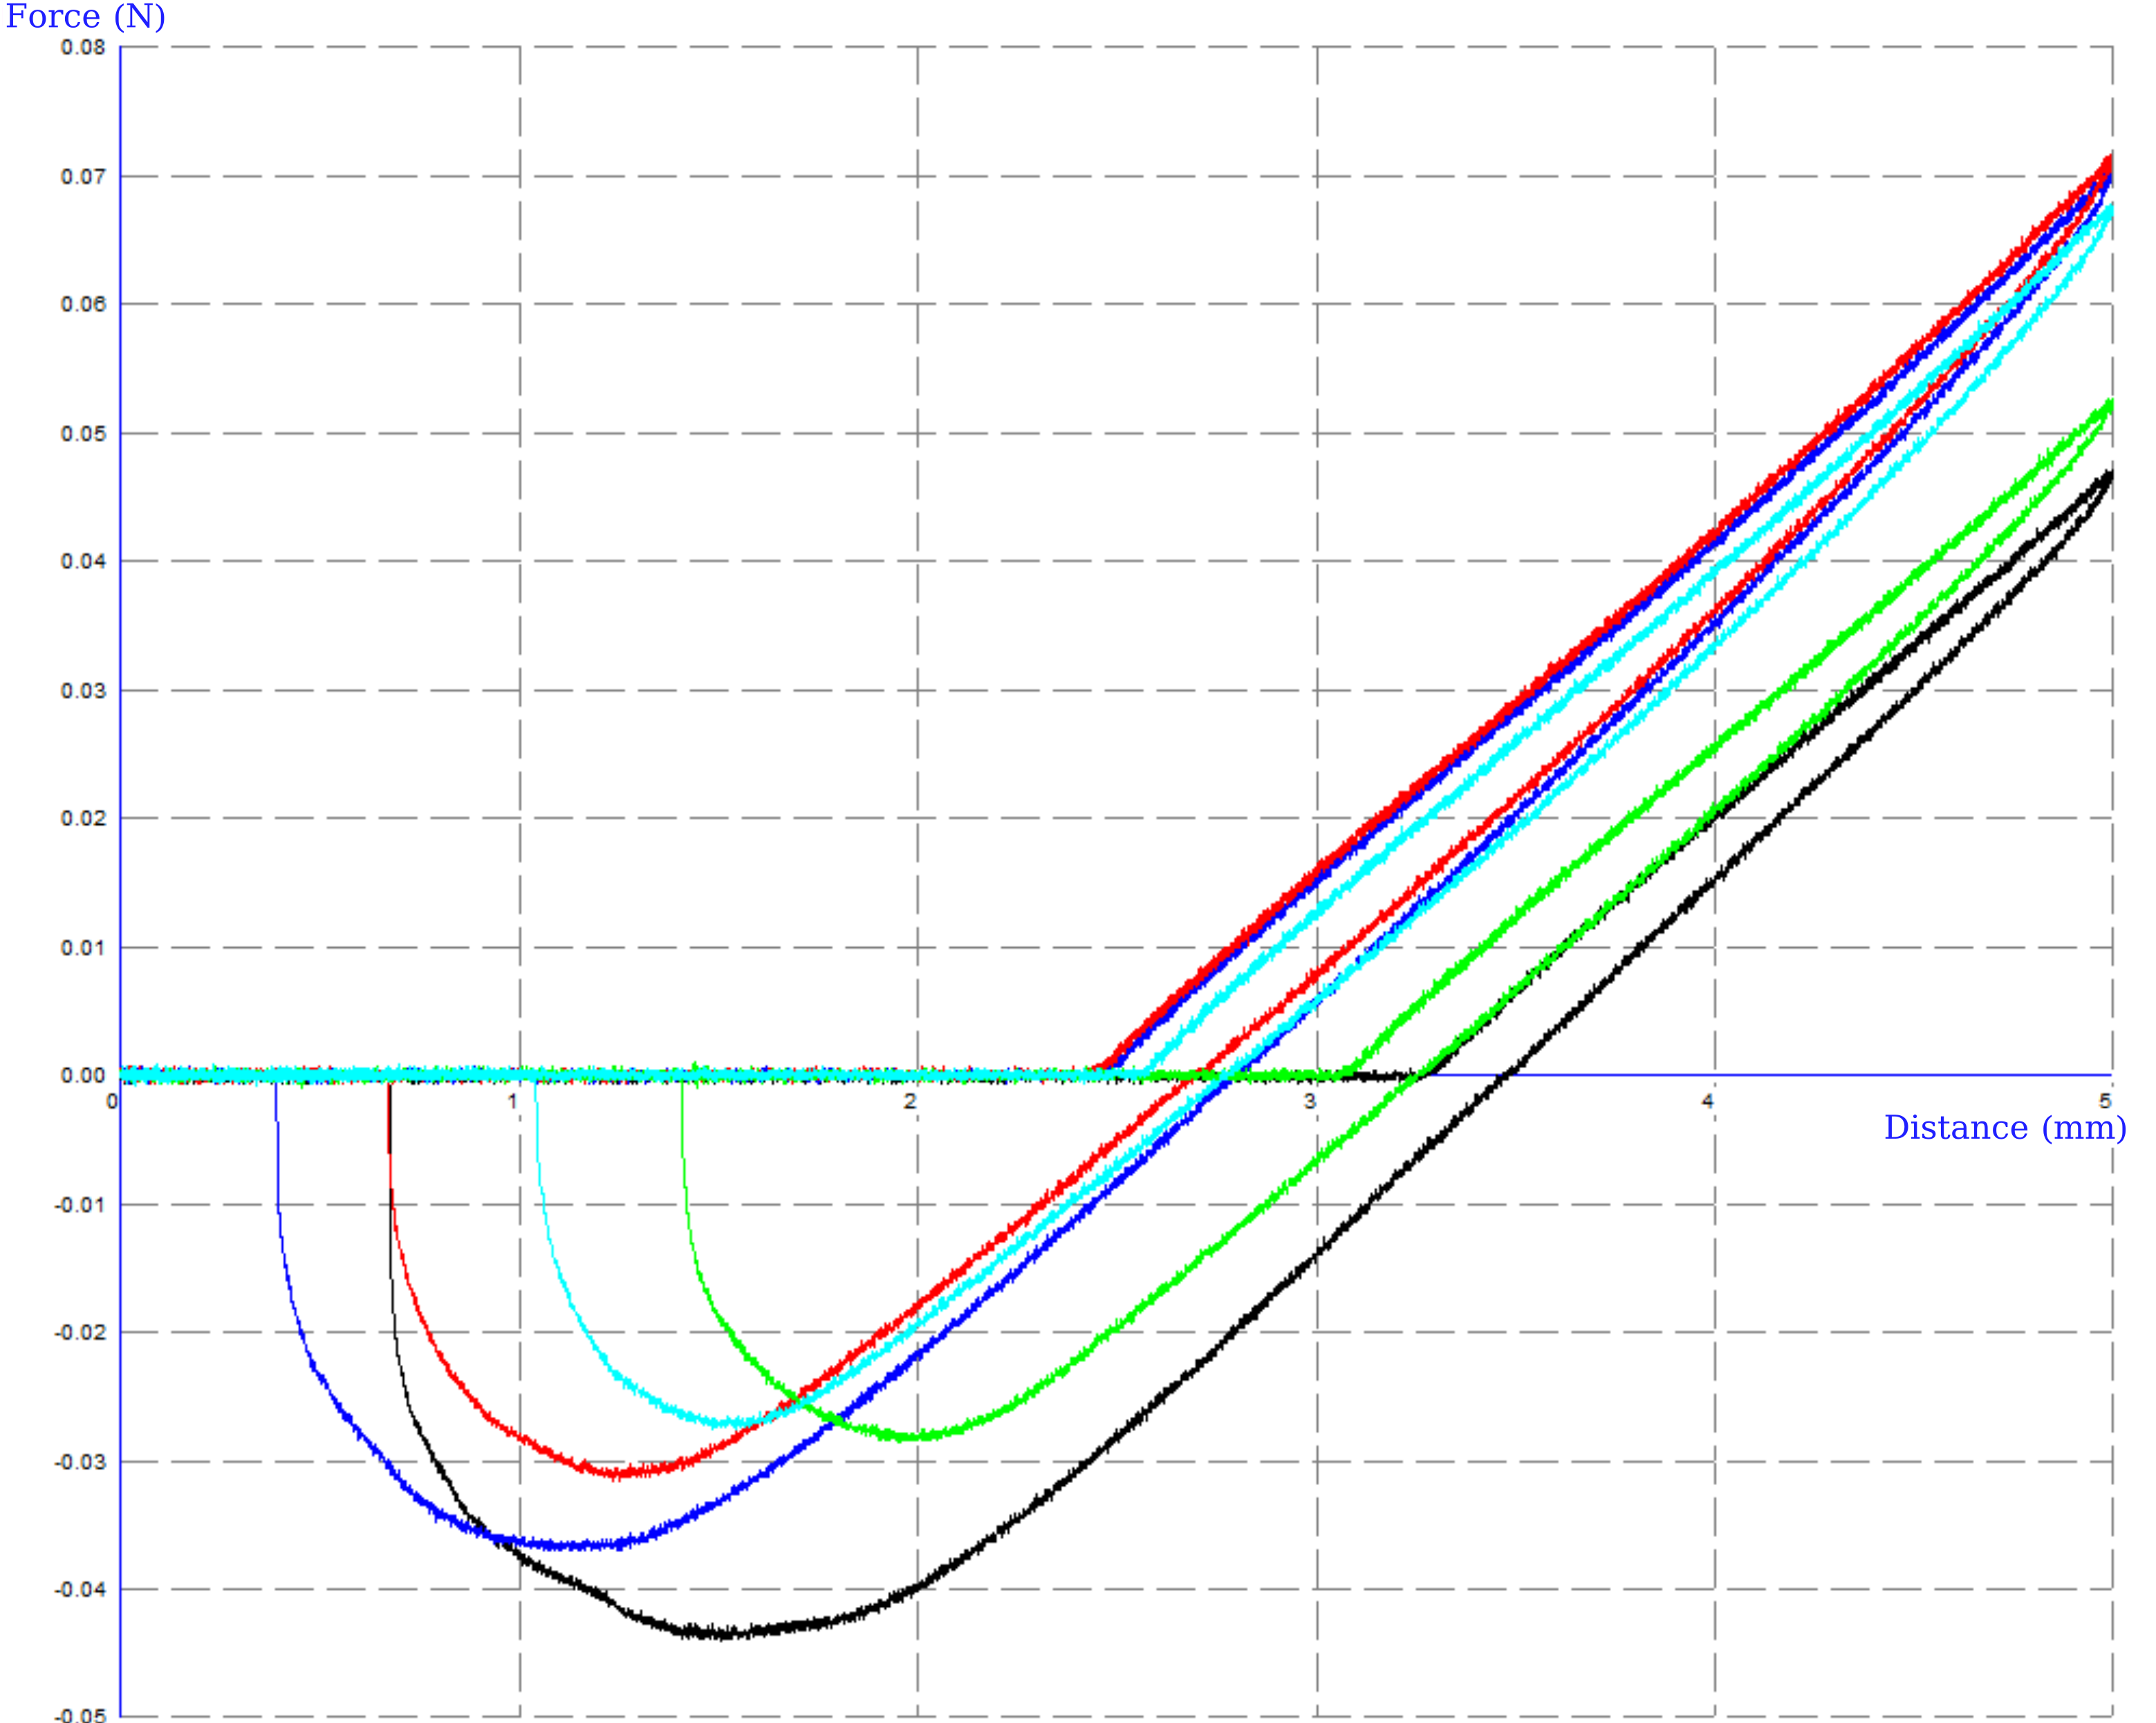
\includegraphics[width=\linewidth]{Chapters/Figures/190406_DC_1-1RT1-5.png}
	\caption[Bulk Modulus Test]{Force vs indentation depth for a bulk sample of silicone. Each color representats a separate measurement at varying starting heights and locations on the sample.\todo[inline, color=pink]{Do you think the axis values are too small? I haven't seen this printed yet.}}
	\label{fig:Bulkstiffness_raw}
\end{figure}

\subsection{Hertzian Contact Mechanics Derivation?}
We calculate the Young's modulus for the bulk sample using classic Hertzian Contact mechanics between a flat, rigid cylinder and an elastic half-space.

\begin{equation}
F=2RE^*d
\end{equation}

where 
\begin{equation*}
\frac{1}{E^*} = \frac{1-\nu_1^2}{E1} + \frac{1-\nu_2^2}{E2}
\end{equation*}
For Silicone, $ \nu \approx .5$ for low strains; for the rigid cylinder, $ E \gg 1-\nu^2 $, so we can ignore that term. From the Force vs. depth information, we can write an equation for E.

\begin{align}
\frac{1}{E^*} &= \frac{2Rd}{F} \\
\frac{1 -\nu^2}{E} &= \frac{2Rd}{F} \\
E &= \frac{\left( 1-\nu^2 \right) F}{2Rd} \\
E &= \frac{\left( 1-.5^2 \right) F}{2(1.5 \cross 10^{-3})d}
\end{align}
\todo[color=pink]{Equation alignment doesn't look right}


\section{Putting it all Together}
Using the texture analyzer, we can measure $ E $ and $ \nu $ for our substrate. We can then use confocal fluorescent microscopy to measure $ d $ vs. $ R $ for many sphere per sample. We can then run a two parameter fit using this Equation \ref{THEeqn} to determine $ \Upsilon $ and $ W $. Using our equibiaxial stretching apparatus, we can repeat the $ d $ vs. $ R $ measurements at a range of strain to determine $ \Upsilon(\epsilon) $. The process of collecting the $ d $ vs. $ R $ measurements for a single sphere is explained in Chapter 3.

%

\chapter{Data Acquisition and Image Analysis}

%Not really sure what this pdf is, but I like it, and will post the link so I don't forget about it https://spie.org/samples/TT69.pdf
\section{Fluorescent Confocal Microscopy} \label{ch:microscopy}
Confocal Microscopy is a technique capable of probing a sample with true 3-Dimensional optical resolution. The technique works by only allowing in focus light through a pinhole. By changing the plane of focus, one can traverse an object azimuthally or reconstruct a full three-dimensional image by compiling a ``stack'' of these images.  

\begin{figure}[h!]
	\centering
	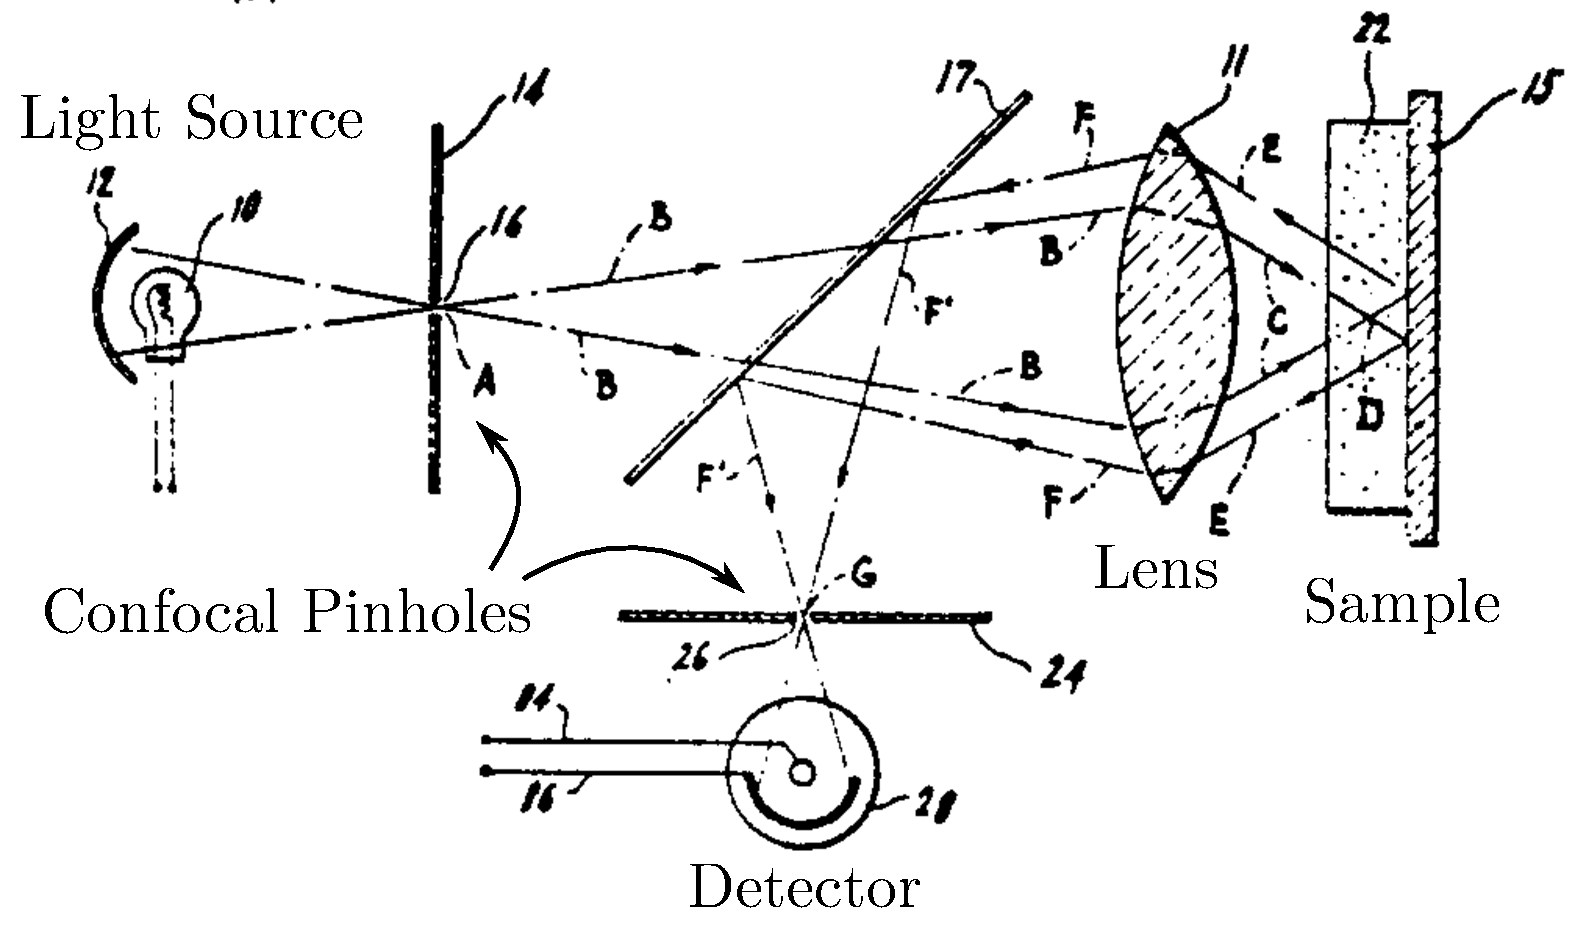
\includegraphics[width=\linewidth]{confocal_stuff/confocalpatent_crop2}
	\caption[Minsky Patent Diagram]{Above is a diagram from Marvin Minky's classic 1961 patent \cite{patent:3013467} for a confocal microscope. A pinhole before the photodetector blocks the out of plane light.}
	\label{fig:confocalpatent}
\end{figure}


\begin{wrapfigure}{r}{.5\textwidth}
	
	\centering
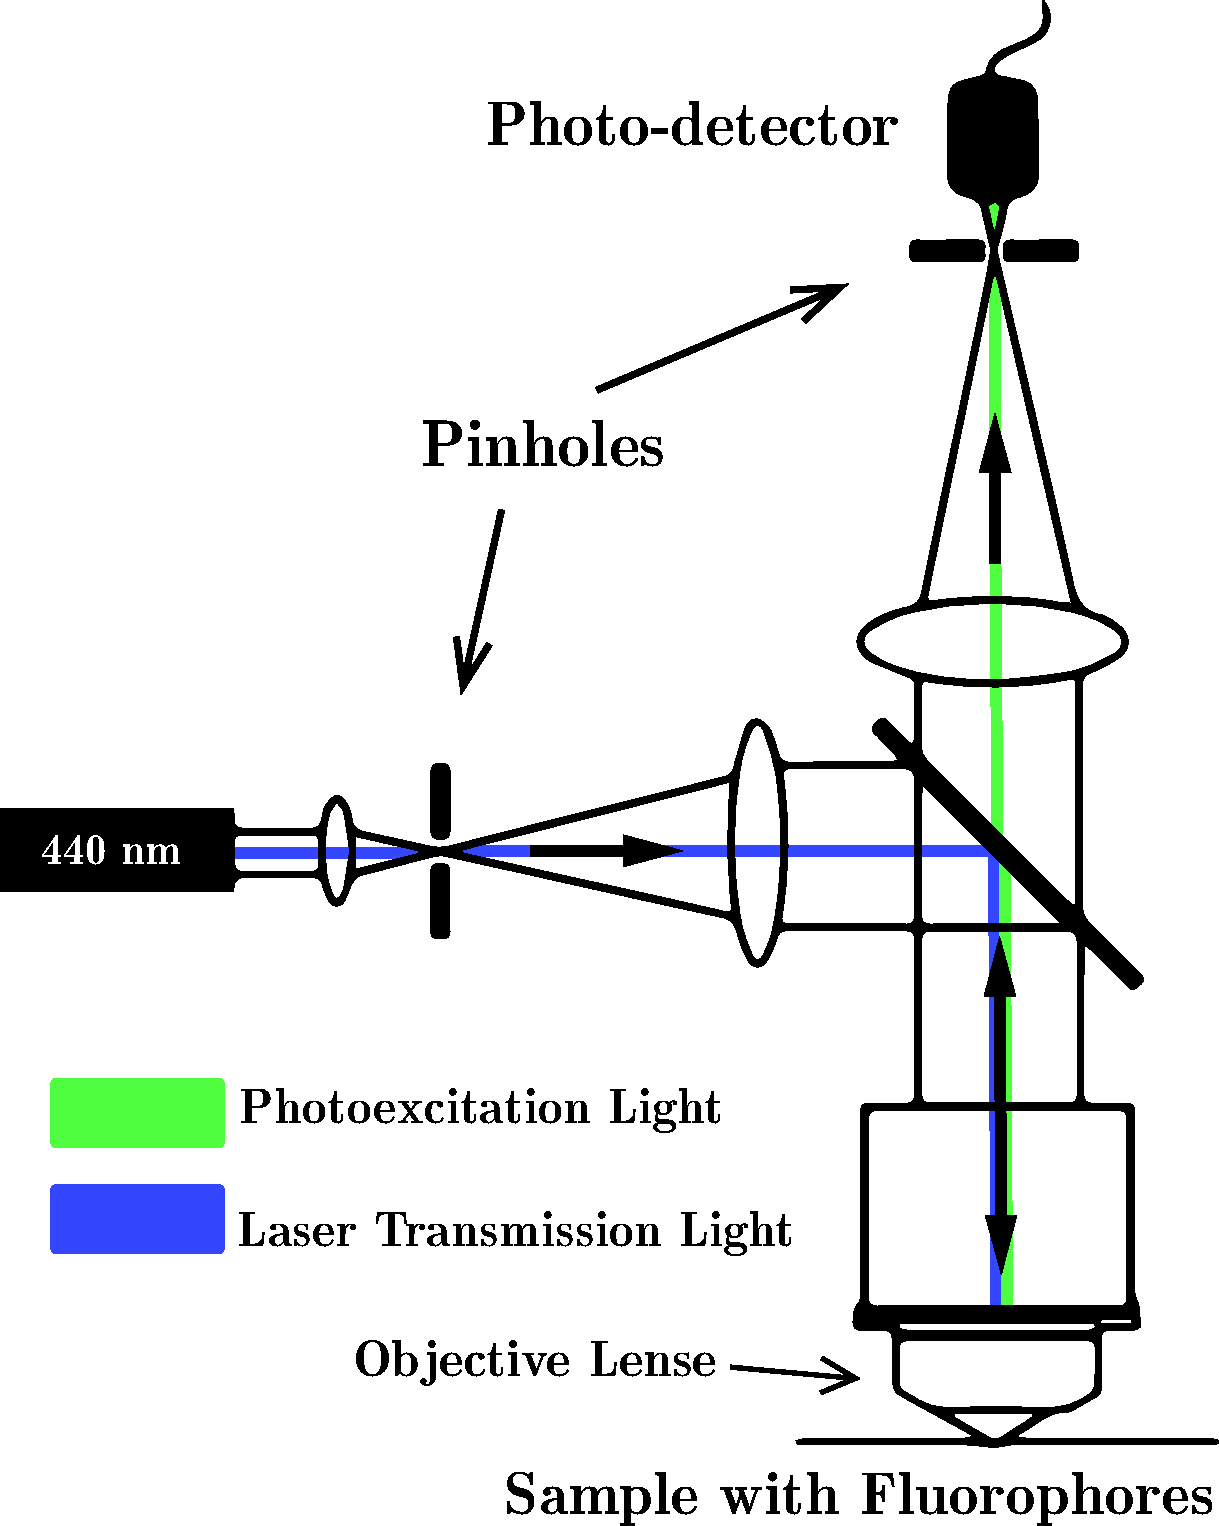
\includegraphics[width=\linewidth]{Chapters/Figures/confocal_fluorescent_diagram_b}
\caption[Fluorescent Confocal Microscopy]{In fluorescent confocal microscopy, a diachroic mirror is used to separate the laser light from that emitted by the excited fluorophores. }
\label{fig:confocalfluorescentdiagram}
	
	
\end{wrapfigure}
	
Fluorescent Confocal Microscopy works by the same general principle, only with the added complexity of optically-excitable fluorophores. These fluorophores absorb light from a narrow range of frequencies and re-emit fluorescent light at a different known and specific frequency, which can then be measured. This allows for a greater resolution to larger objects, as well as the ability to detect objects that would otherwise be invisible to the microscope.  

Fluorescent Confocal Microscopy works by illuminating the specimen with a laser. The laser light passes through a pinhole, then is reflected by the dichroic mirror and then focused by the objective lens on a small area of the specimen. The re-emitted light from the fluorophores has a longer wavelength than the laser, so it is then transmitted through mirror.  It then then passes through the pinhole where it is travels to the photodetector. A diagram of this process can be found in figure \ref{fig:confocalfluorescentdiagram}.
%\begin{figure}[h!]
%	\centering
%	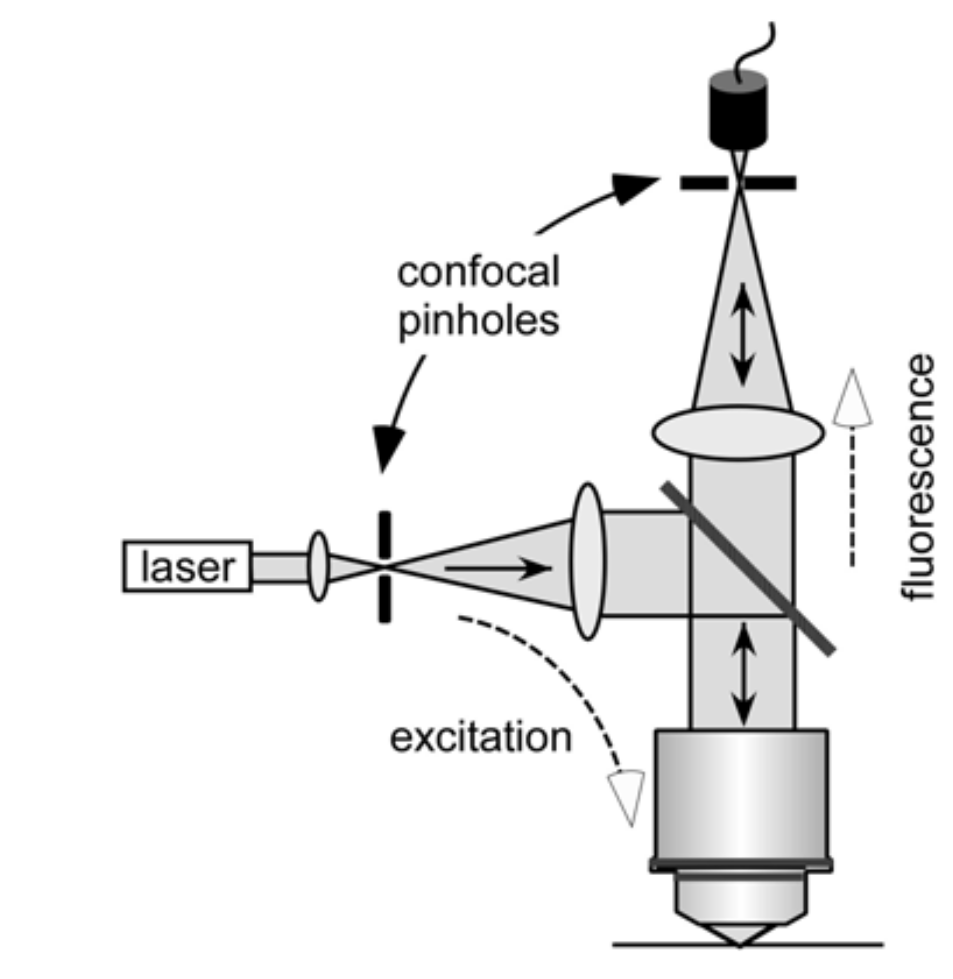
\includegraphics[width=\linewidth]{Chapters/Figures/confocal_fluorescent_diagram}
%	\caption[Fluorescent Confocal Microscopy]{In fluorescent confocal microscopy, a diachroic mirror is used to separate the laser light from that emitted by the excited fluorophores. }
%	\label{fig:confocalfluorescentdiagram}
%\end{figure}

\section{Applying Fluorescent Confocal Microscopy to the Sample}
In order to see our substrate with fluorescent confocal microscopy, we need to coat the surface of our substrate with tiny fluorescent beads (fluorophores) on the order of 40nm in radius. The detection of these fluorescent beads allows us to see the outline of the substrate's surface, as well as the indenting sphere, which displaces the beads beneath it as in sinks into the substrate. Directions for preparing a fluorescent bead solution in a borate buffer can be found in Appendix section \ref{appendix_beads}. 

\subsubsection{Fluorescent Confocal Microscopy Data Collection}
Data was obtained using the Nikon A1R+ Confocal Microscope. To take image stacks of the Fluorescent beads, we use a 50x water-immersion objective lens. We set the laser to 440nm and adjust the power (HV) and gain as needed. Generally these values are around 5.0\% and 40 Volts, respectively. In order to get clear locating, it is important not to saturate the photo-detector. 

\begin{figure}
	\centering
	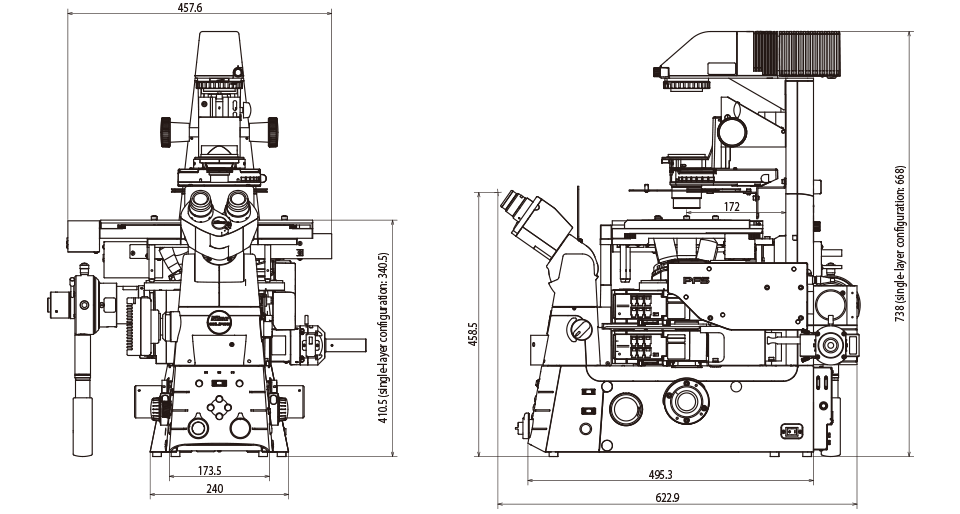
\includegraphics[width=0.8\linewidth]{confocal_stuff/Ti2_diagram_1}
	\caption[Nikon Ti2 Microscope Base]{This may only be here because it's pretty....Also, I'd like to remove the measurements when I have time. Also, not sure how to cite the manual yet.}
	\label{fig:ti2diagram1}
\end{figure}

For silica spheres ranging from $5-50$ $\mu$m in size, we have found the best scaling factor to be $.104$ $\mu$m/pixel in the horizontal plane for an image of 1024 $ \cross $ 1024 resolution. We set the vertical step size (z-direction) to $.225$ $\mu$m/px or $.25$ $\mu$m/px depending on what the confocal recommended. Both provided adequate vertical resolutions. 16x averaging using the resonant scanner took up to 5 minutes per scan, but provided excellent resolution. 

\subsection{Raw Data Files}
Using confocal microscopy, we collect a ``stack'' of images, detecting the light from the fluorescent beads. Below (Fig. \ref{fig:190215g91glasssphere011surface}) is a raw data image of the surface of a soft substrate with a glass bead stuck below.

\begin{figure}[h!]
	\centering
	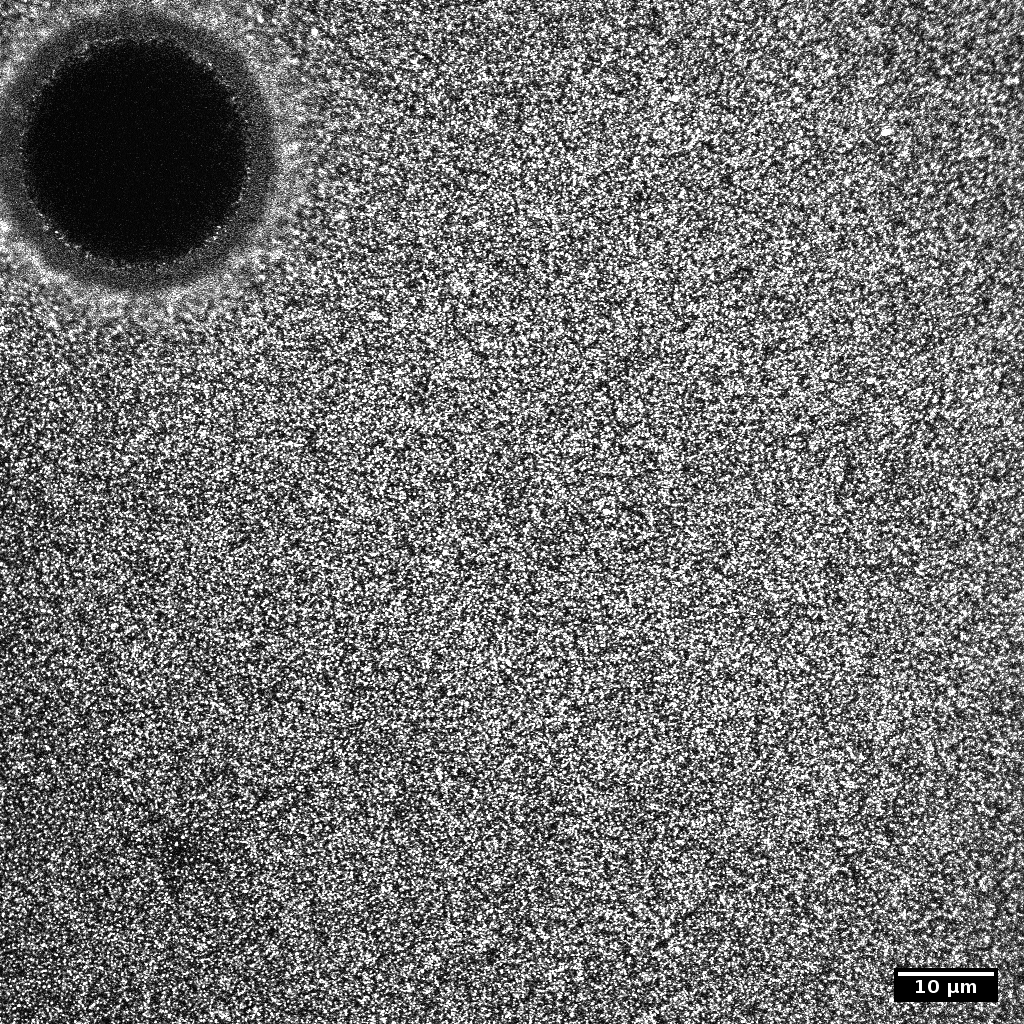
\includegraphics[width=.75\linewidth]{Chapters/Figures/190215_g91_glass_sphere011_surface.png}
	\caption[The surface plane of a silica bead in silcone]{The surface plane of a silica bead in Gelest 9:1 Silicone (E = 7.3 kPa). Radius of sphere = 28.7 $\mu$m.}
	\label{fig:190215g91glasssphere011surface}
\end{figure}
The object resembling a black hole in the top-left corner is the silica sphere. Each small white dot represents a fluorescent bead; together they create a sea of stars that outline the surface plane and the silica sphere. Figure \ref{fig:190215g91glasssphere011surface} is an example of the upper limit of bead coverage density. Any higher concentration of fluorescent beads could result in a difficulty in light bleeding. Note, the sphere is in the top corner of the image to provide maximum information about the leveling of the surface plane. We assume that the surface effects are symmetrical for zero applied strain and equibiaxial strain. Thus, it is more important to gather information in one direction to properly level the surface plane to determine the depth into which the sphere sinks. 

For each sphere, we take a stack of 50-100 images, depending on the size of the sphere. Figure \ref{fig:sphere011cascade} shows several vertical slices from the bottom of the sphere to just above the surface of the substrate.\todo[inline,color = pink]{wrong auto fig ref?}

\begin{figure}[h!]
		
	\begin{tabular}{ccc}
		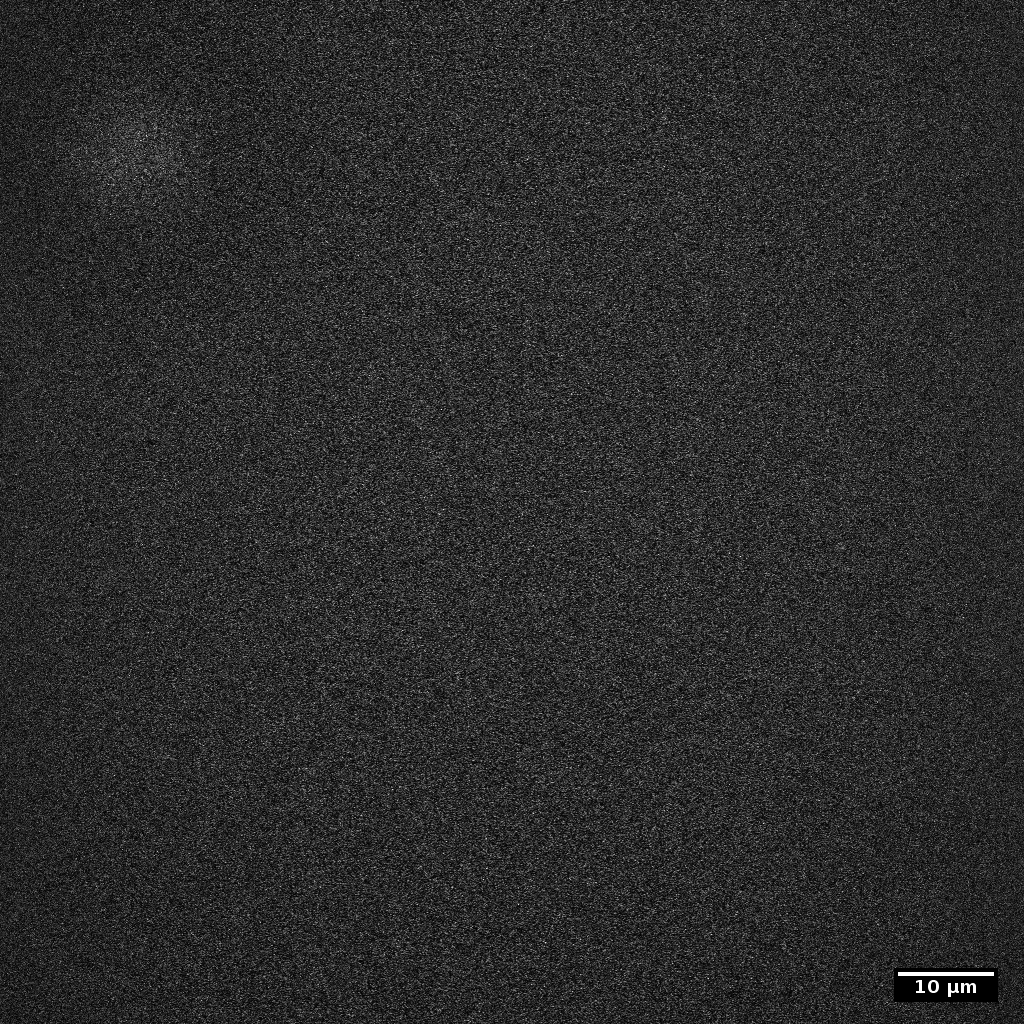
\includegraphics[width= .33\linewidth]{Chapters/Figures/190215_g91_glass_sphere011_cascade1.png} & 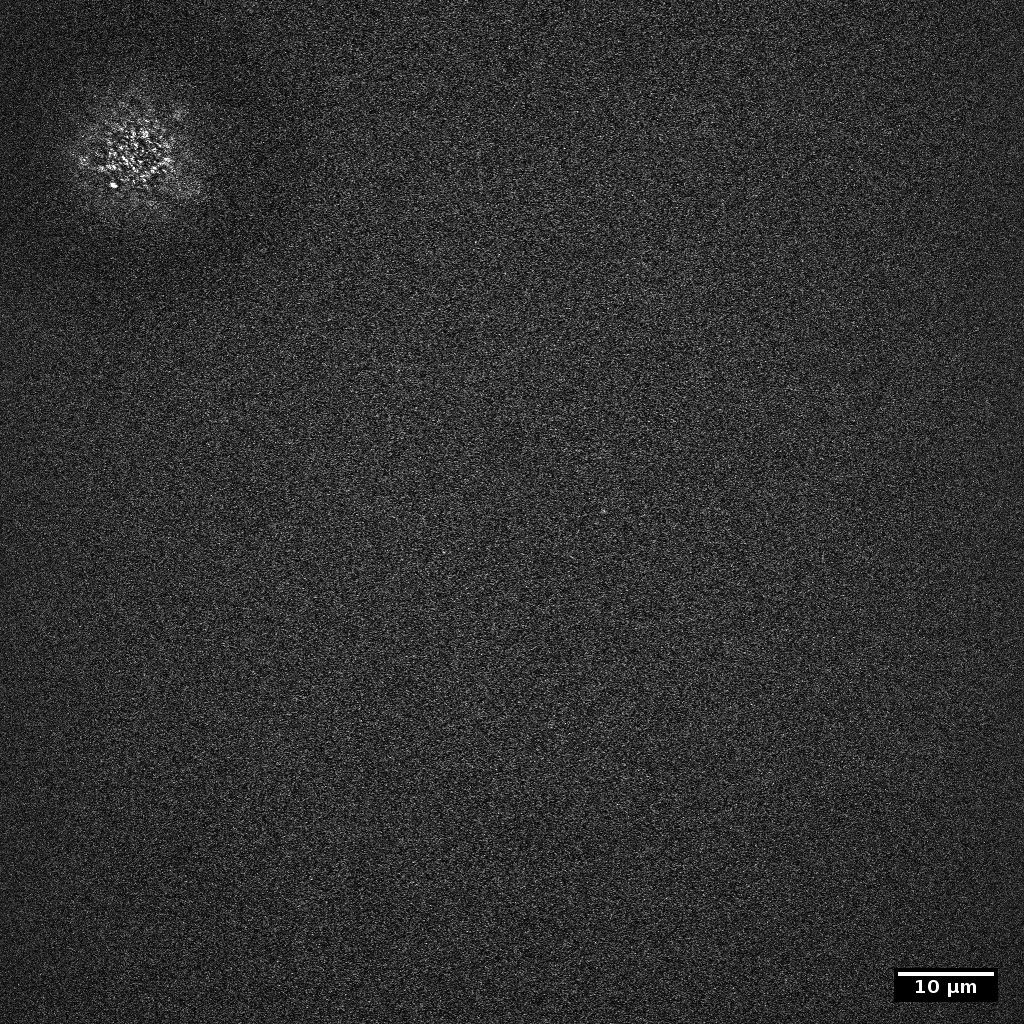
\includegraphics[width= .33\linewidth]{Chapters/Figures/190215_g91_glass_sphere011_cascade2.png} & 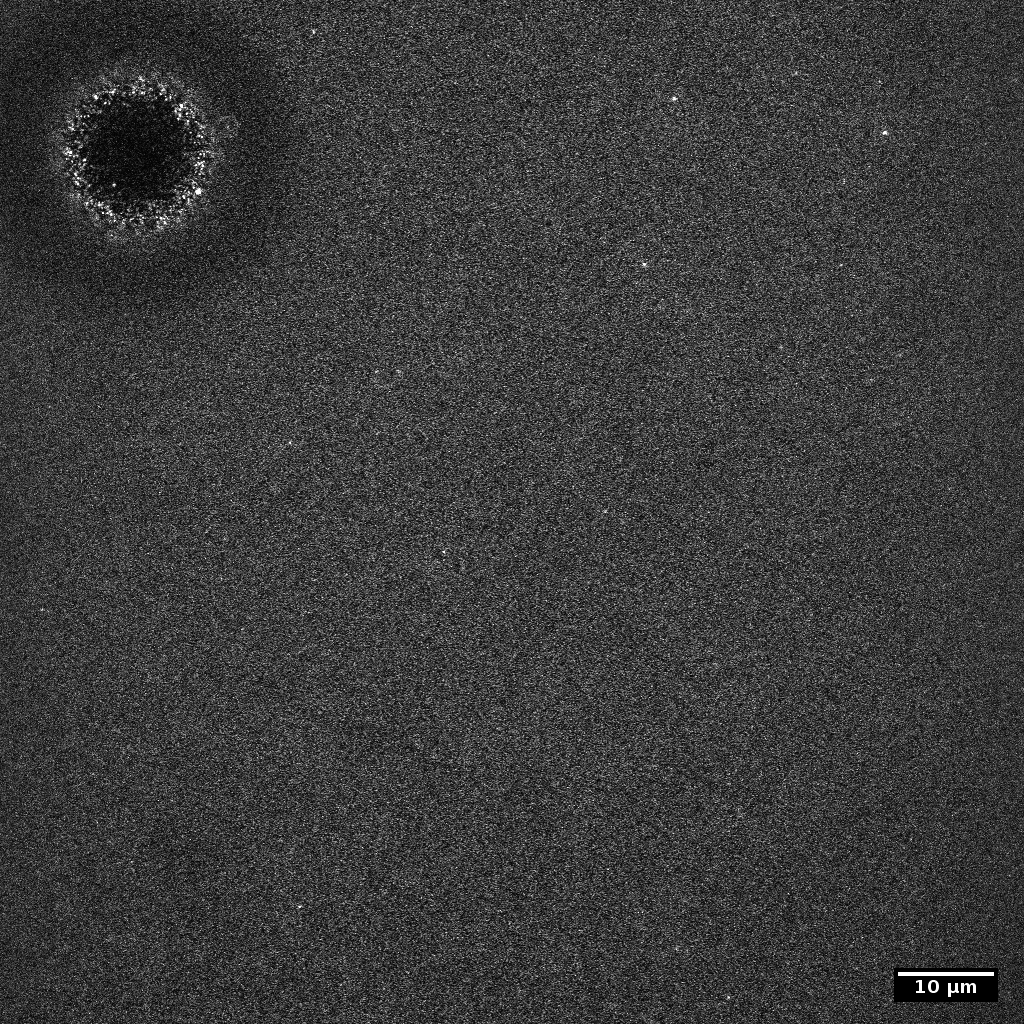
\includegraphics[width= .33\linewidth]{Chapters/Figures/190215_g91_glass_sphere011_cascade3.png} 
		\\
		a) & b) & c) \\
		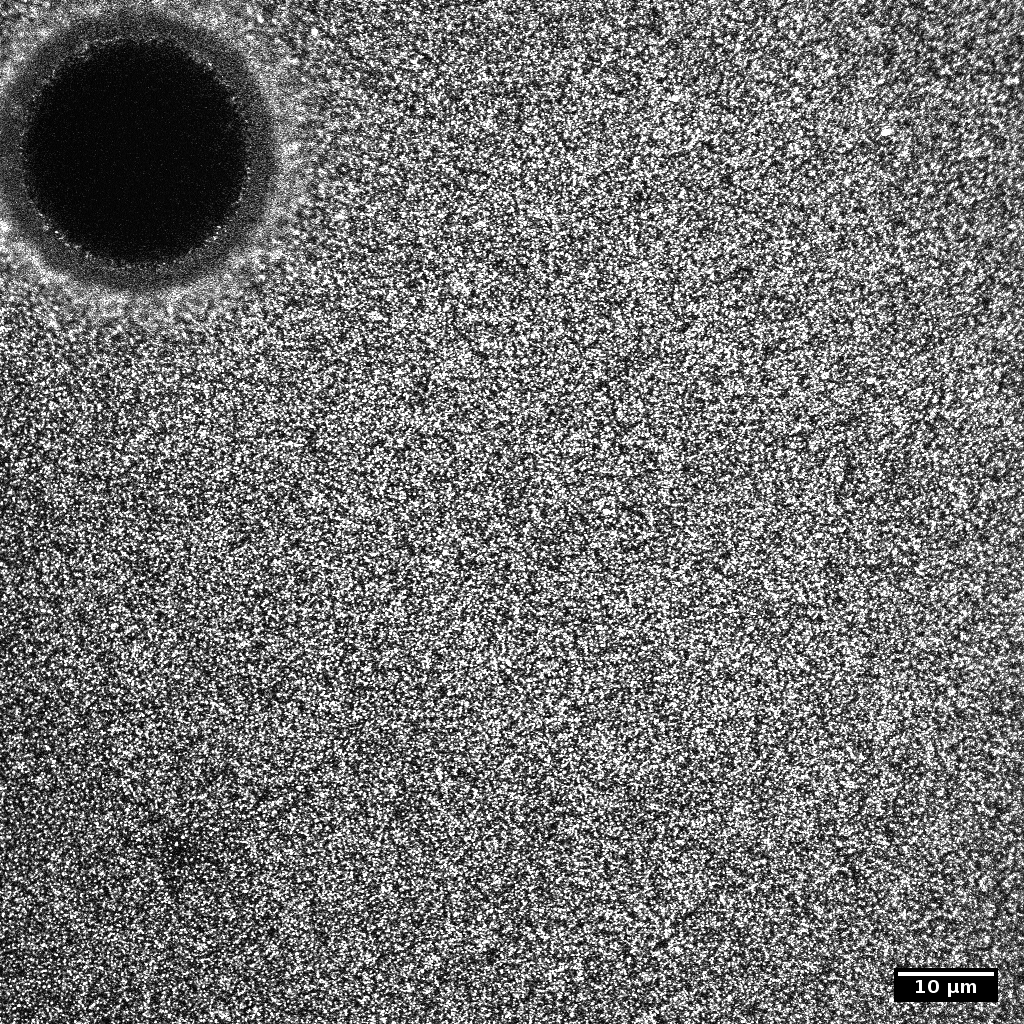
\includegraphics[width= .33\linewidth]{Chapters/Figures/190215_g91_glass_sphere011_cascade4.png} & 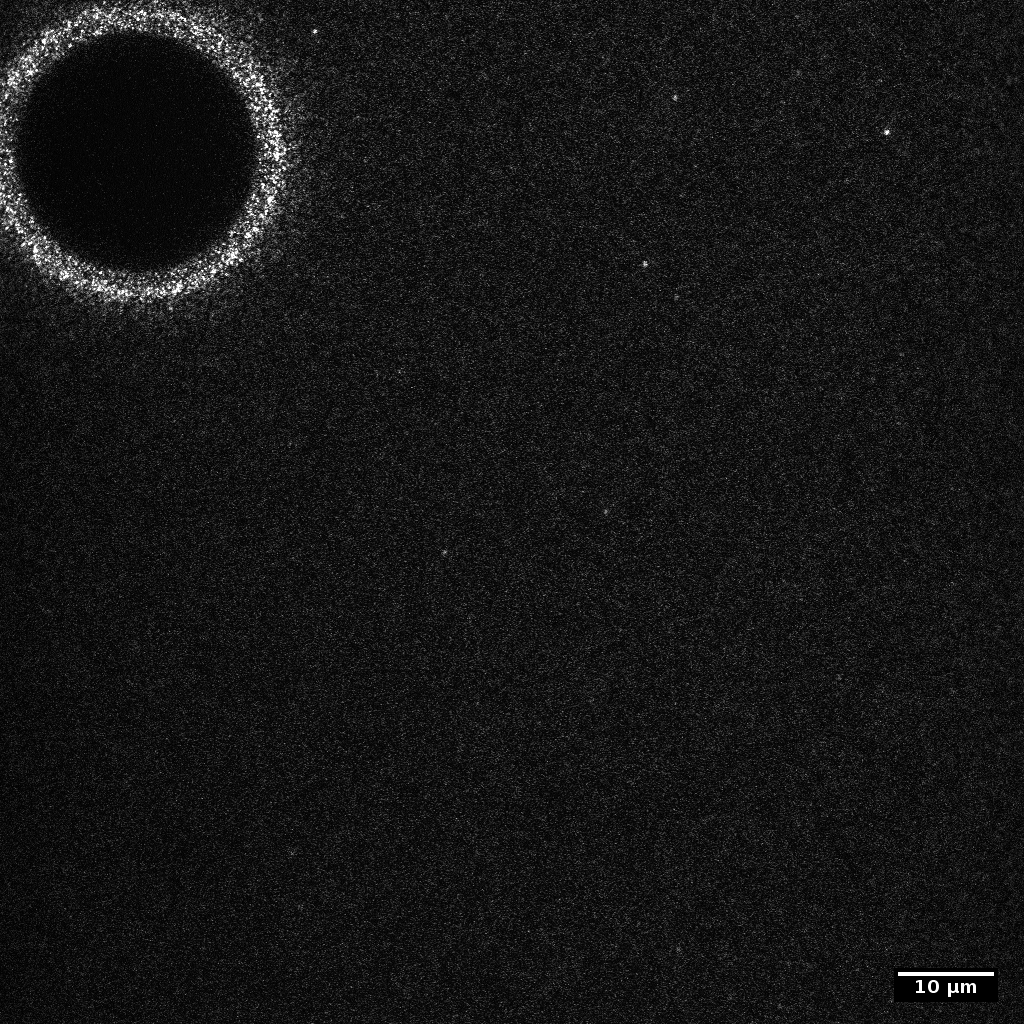
\includegraphics[width= .33\linewidth]{Chapters/Figures/190215_g91_glass_sphere011_cascade5.png} & 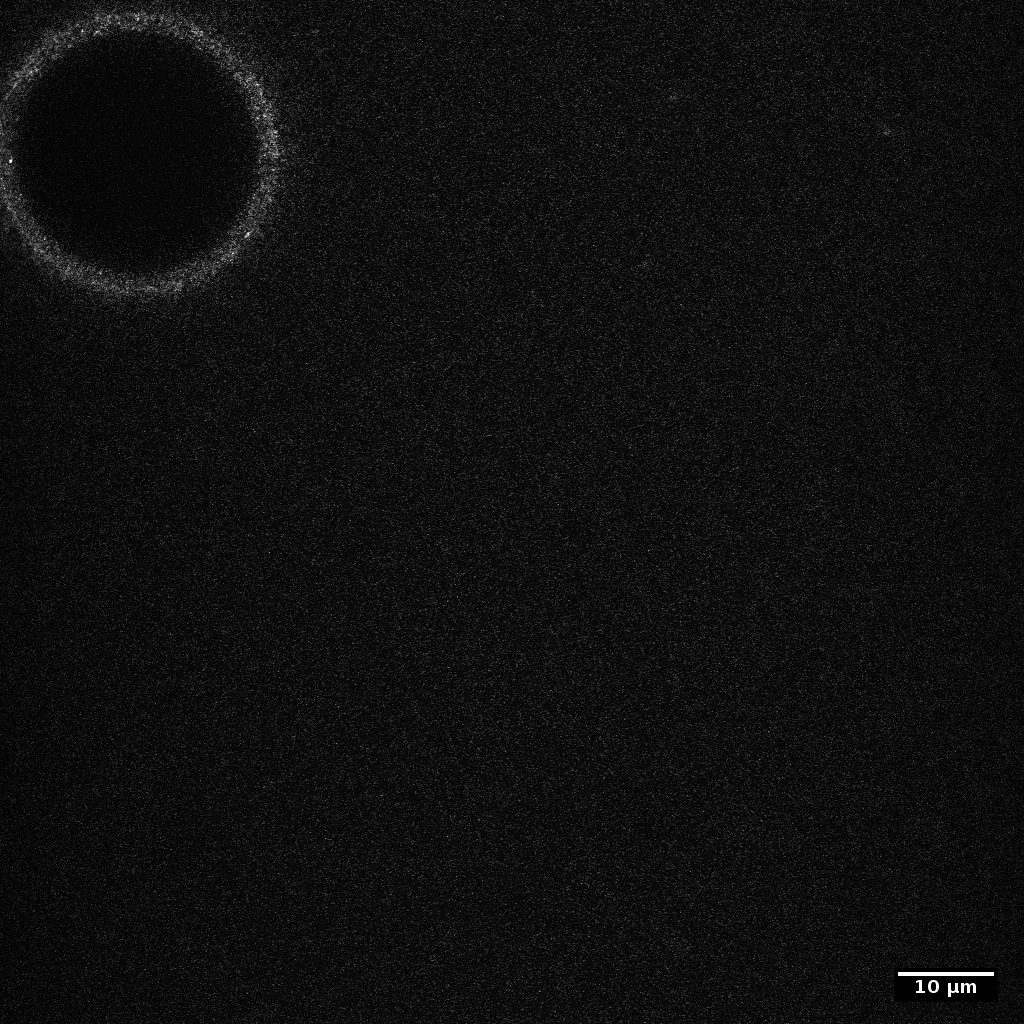
\includegraphics[width= .33\linewidth]{Chapters/Figures/190215_g91_glass_sphere011_cascade6.png}
		\\
		d) & e) & f) \label{fig:sphere011cascade}
	\end{tabular}
	\caption[Vertical path through image stack]{Images a-f display the x-y plane of the same sample traversing vertically from below the silica sphere to above the surface plane. The scale bar in the bottom right corners represent 10 $\mu$m.}
\end{figure}


\section{Image Analysis}
In the following section, we will step through the process of analyzing a single sphere. Recall that in order to determine the surface stress and adhesion energy, we must fit equation \ref{THEeqn} to the depth vs. radius measurements for a collection of spheres.  

\subsection{Particle Location}
To turn a raw image file (saved as a .ome.tif) into usable data, we use a MATLAB program to locate each fluorescent bead. This is plotted in Figure \ref{fig:particlelocatednormalized}. The flat orange plane of points is the surface, and the dark blue are the fluorescent beads pushed underneath the microsphere as it sinks into the substrate. It is easy to see the outline of the microsphere, and we can use this information to determine d and R for the sphere. 
Figure \ref{fig:particlelocatedstretched} shows the same sphere but stretched in the vertical axis to see the fluorescent bead density towards the bottom of the sphere. 
\begin{figure}[h]
	\centering
	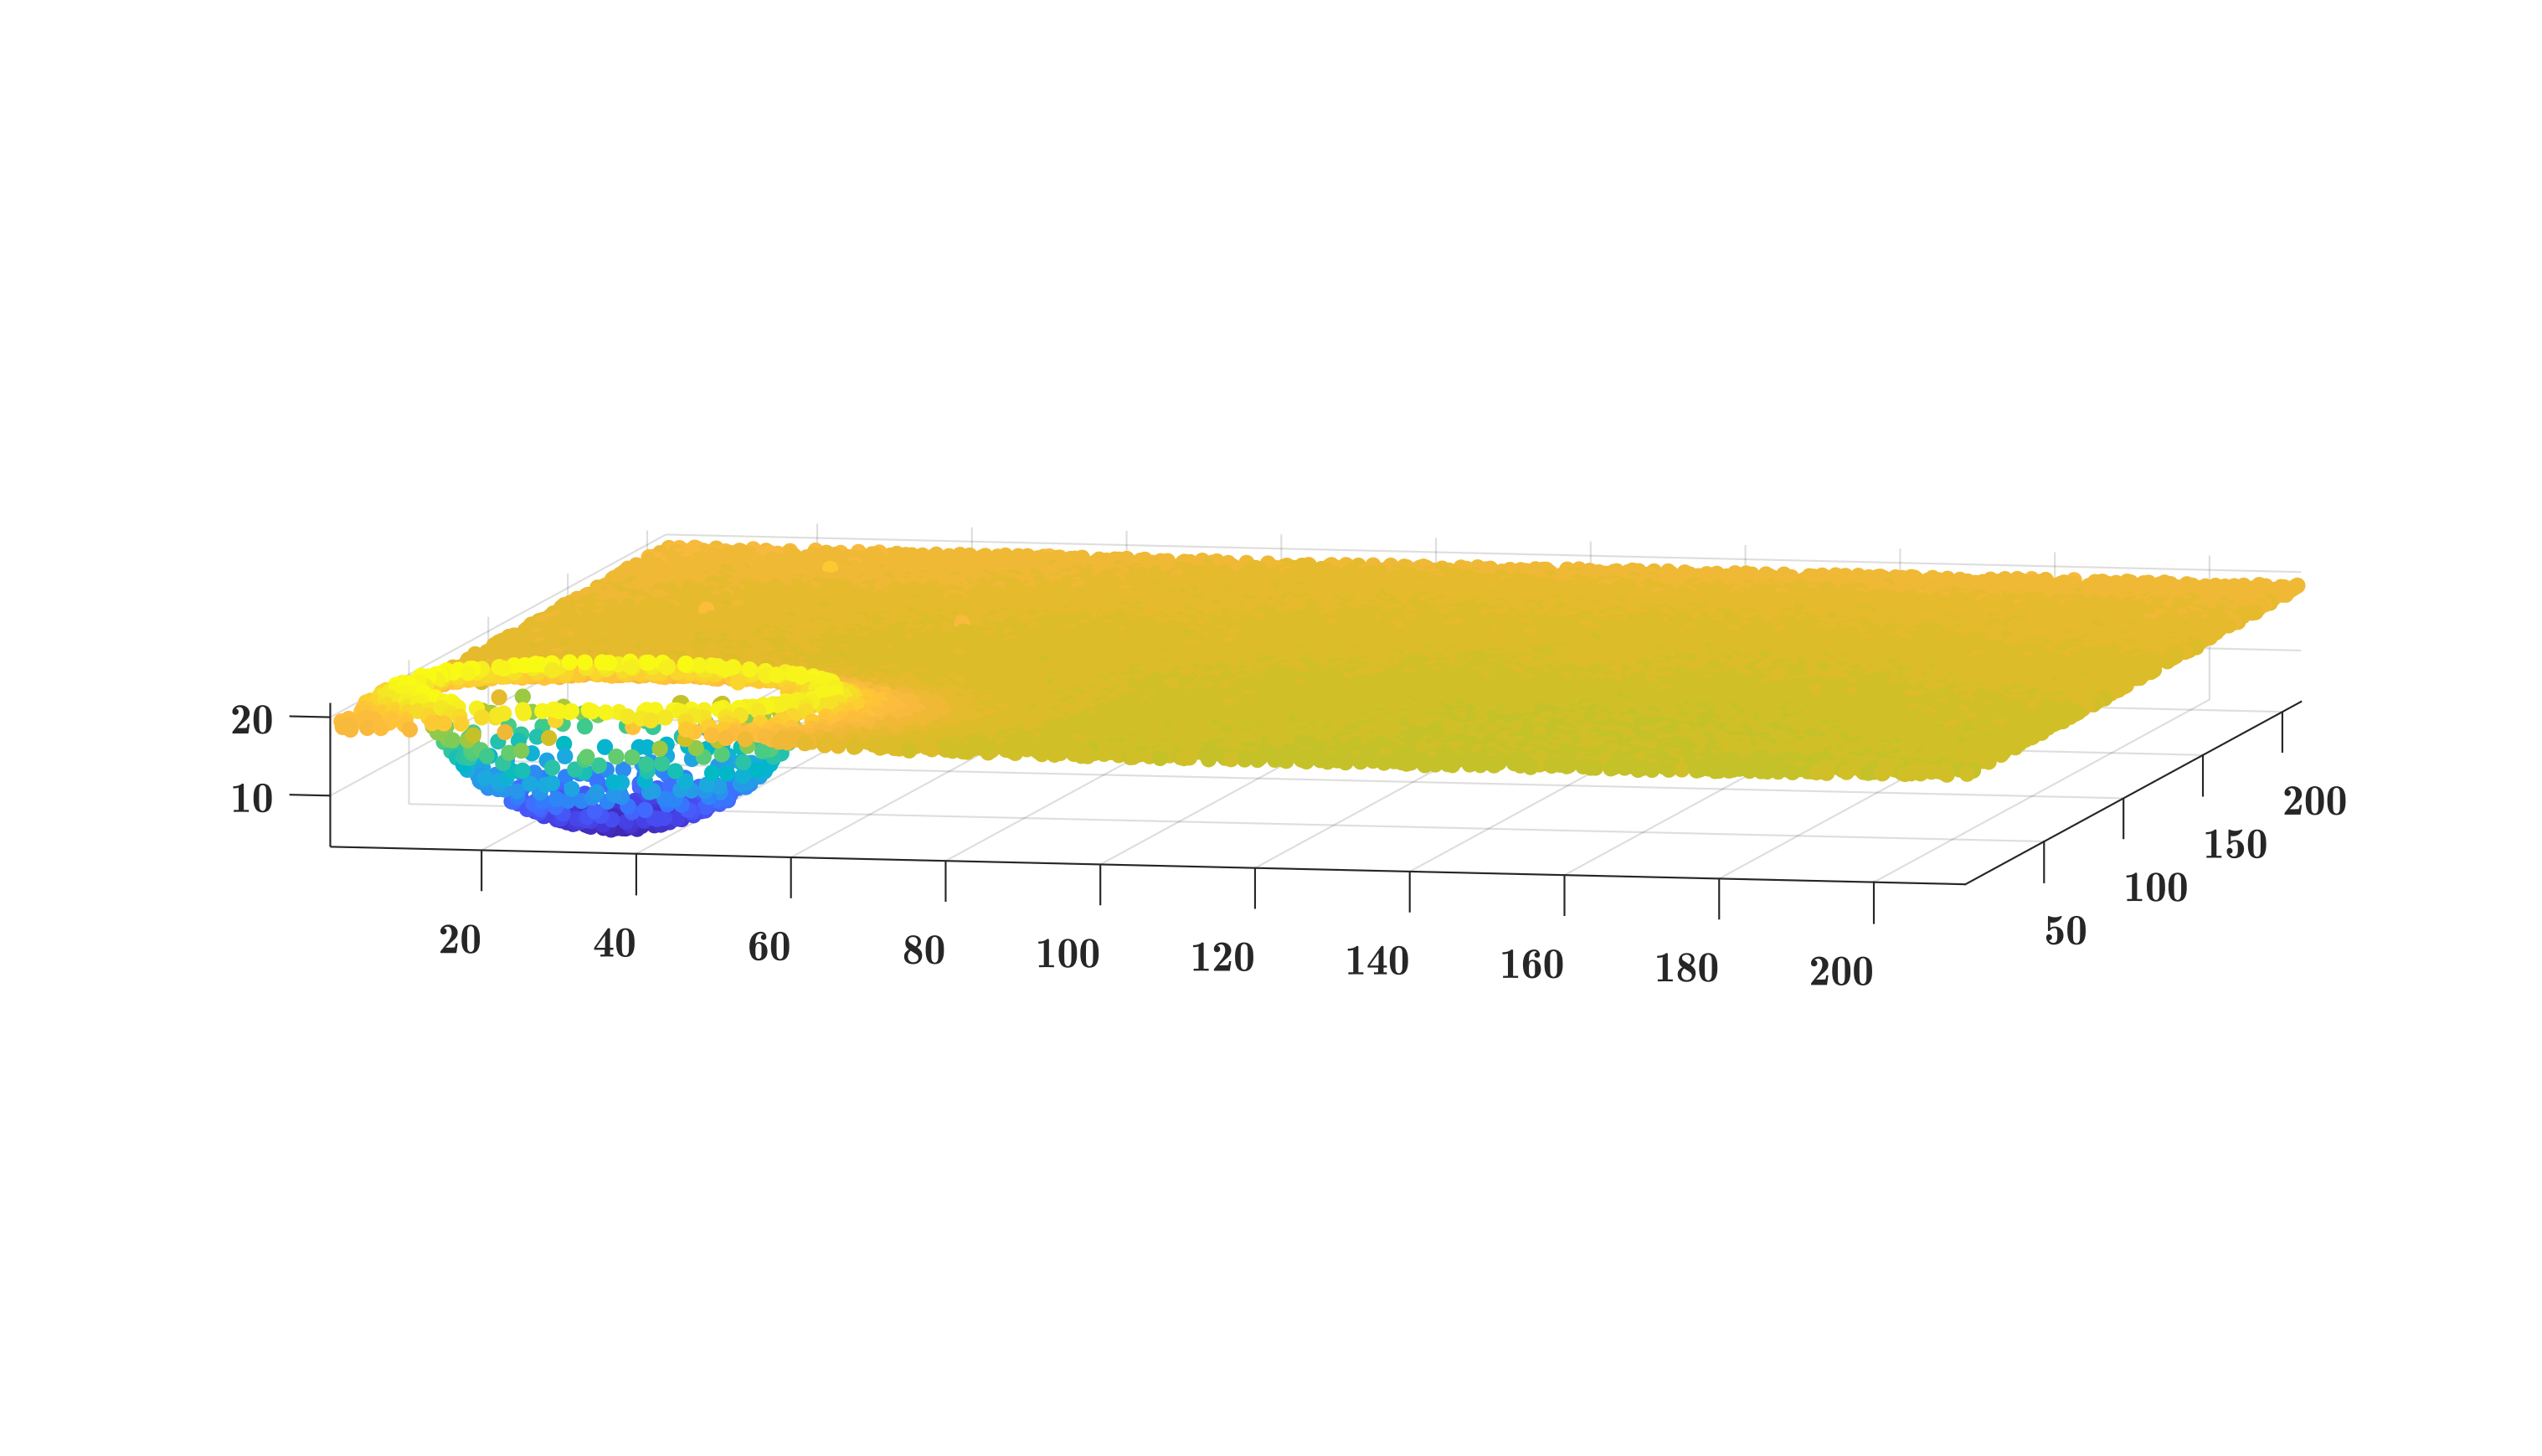
\includegraphics[width=\linewidth]{Chapters/Figures/sphere011_ia/particle_located_normalized}
	\caption[Particle Located: Normalized-Axes]{Using MATLAB sotware, we can locate each of the fluorescent beads in a given image stack. Here, we've plotted the located beads for the same sphere as in Figure \ref{fig:190215g91glasssphere011surface} and \ref{fig:sphere011cascade}. The dense blanket of orange points represents the surface of the substrate, and the blue points are the fluorescent beads pushed beneath the silica sphere during indentation.}
	\label{fig:particlelocatednormalized}
\end{figure}


\begin{figure}[h!]
	\centering
	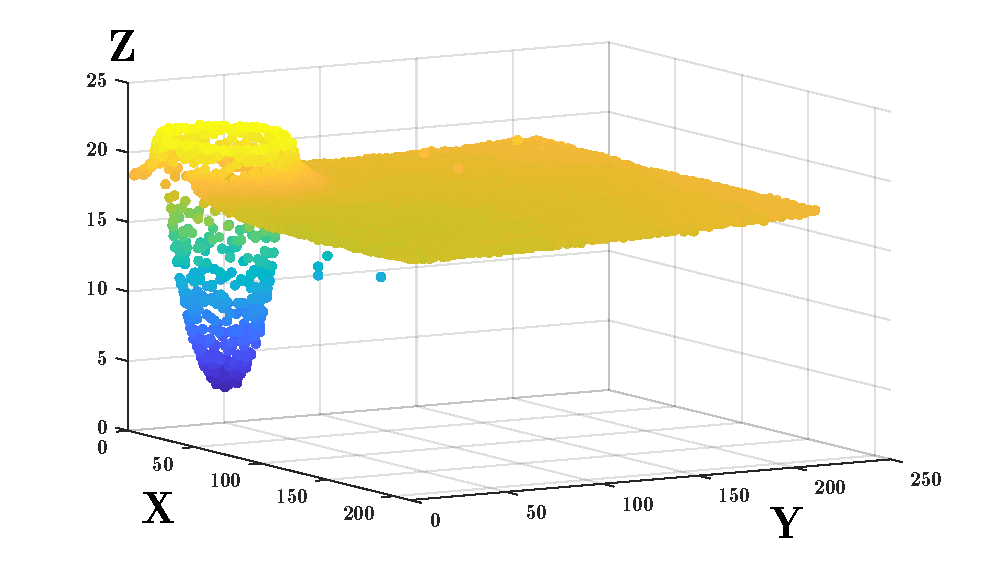
\includegraphics[width=\linewidth]{Chapters/Figures/sphere011_ia/particle_located_stretched}
	\caption[Particle Located: Stretched-Axes]{Fluorescent bead location for the same sphere as Fig.  \ref{fig:particlelocatednormalized}, only now it is stretched vertical axis to showcase the bead density under the bottom of the sphere.}
	\label{fig:particlelocatedstretched}
\end{figure}

\begin{figure}[h]
	\centering
	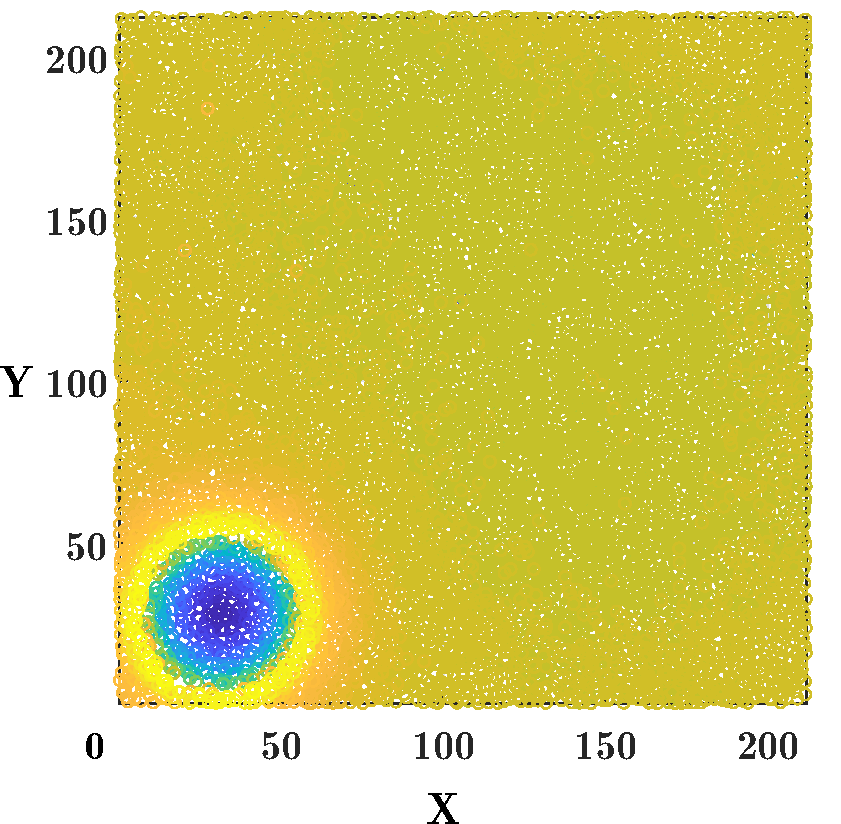
\includegraphics[width=\linewidth]{Chapters/Figures/sphere011_ia/particle_located_top_view}
	\caption[Particle Located: Top View]{Here is the top view of the same sphere as in the previous figures. This allows us locate the center of the base of the sphere. From this we can construct a side profile (\ref{fig:sidecollapsed})}
	\label{fig:particlelocatedtopview}
\end{figure}
\subsection{Depth and Radius Determination}
After locating all the fluorescent beads and reconstructing our raw image in a useful format, we can then use this information to extract the depth and the radius of the sphere. To accomplish this, we first determine the center of out sphere from the top (x-y plane) and collapse the side profile of the \todo{clunky} sphere. Figure \ref{fig:sidecollapsed} depicts the x-z plane as a cross-section through center of the sphere. We only need half of the sphere's profile to fit a circle. This ensures we have a large field of view to properly level and determine the substrate's surface. Figure \ref{fig:sidecollapsedzoomed} provides a zoomed in view of Fig. \ref{fig:sidecollapsed} to better indicate the resolution to which we try to fit a circle. Note the abrupt cut off around 26 $\mu$m and how the substrate is lifted up above the zero-plane due to adhesion. Also notice the flatness on of the substrate between $ ~26-29 \mu $m. Not all sample have this flat ridge; many sphere lift the substrate to a point which the immediately slopes downward back to the zero-plane. This behavior depends slightly on the sphere size, but it is mainly a reflection of the amount of phase-separation induced. This is a property of the each silicone which depends on the environmental conditions. 


\begin{figure}[h!]
	\centering
	\large \textbf{No Applied Strain (On Glass): Large Sphere}\\ \vspace{.4 em}
	\large \textbf{Gelest 9:1 (E=6.3kPa)}
	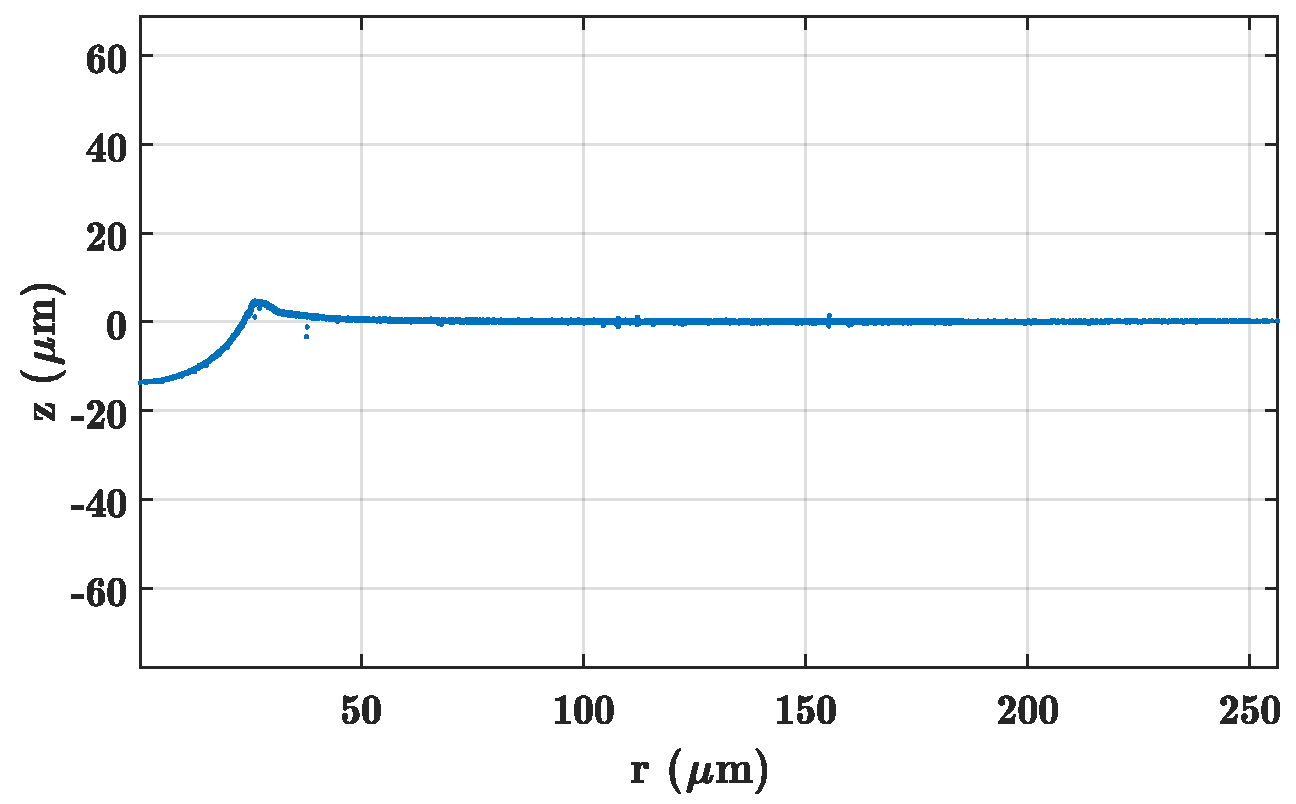
\includegraphics[width=\linewidth]{Chapters/Figures/sphere011_ia/side_collapsed}
	\caption[Collapsed Side Profile]{The constructed image of the outlined sphere with normalized axes. The Axes are in microns.}
	\label{fig:sidecollapsed}
\end{figure}
\begin{figure}[h!]
	\centering
	\large \textbf{No Applied Strain (On Glass): Large Sphere}\\ \vspace{.4 em}
	\large \textbf{Gelest 9:1 (E=6.3kPa)}
	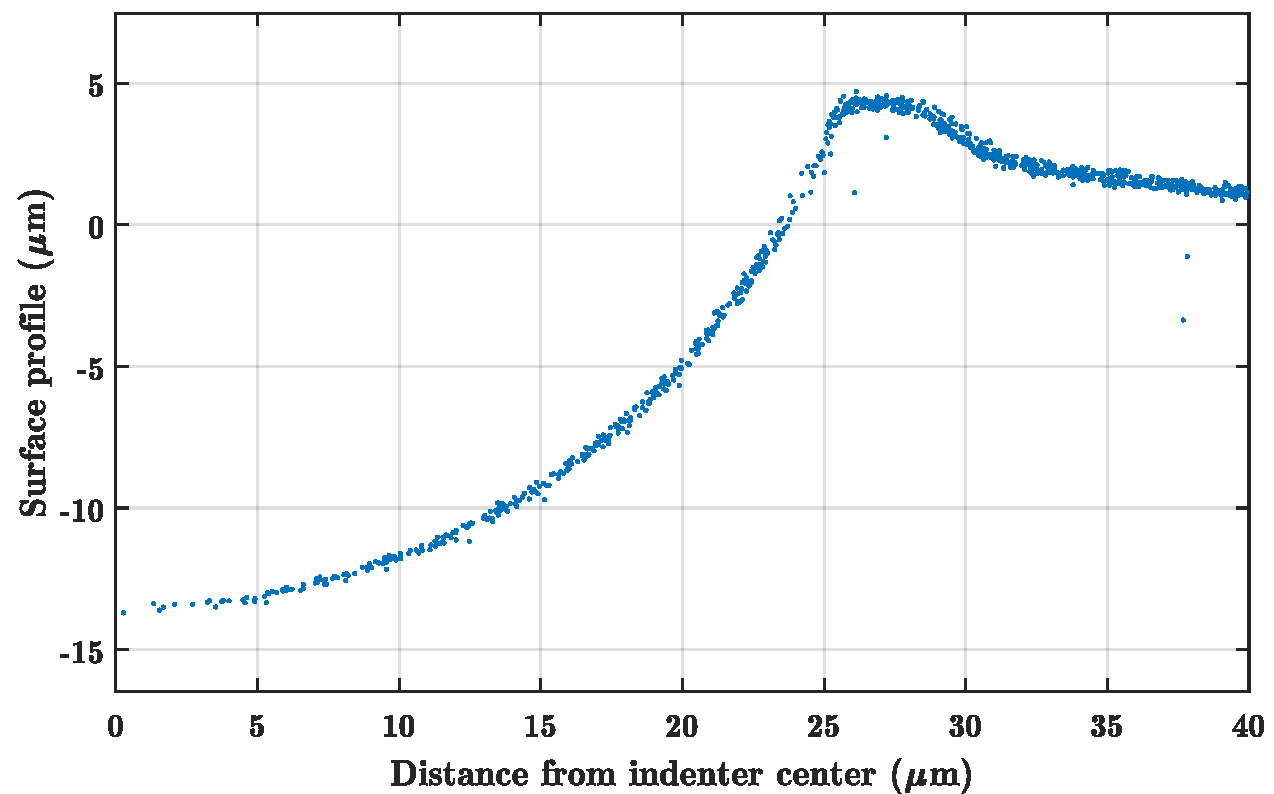
\includegraphics[width=\linewidth]{Chapters/Figures/sphere011_ia/side_collapsed_zoomed}
	\caption[Collapsed Side Profile: Zoomed]{This is a zoomed-in version of figure \ref{fig:sidecollapsed}. It is useful to zoom in and see the the quality of the collapse. A dense collapse leads to a smaller margin of error in fitting a circle to the profile (See Fig. \ref{fig:circlefit}).}
	\label{fig:sidecollapsedzoomed}
\end{figure}

It is important to be careful with the circle-fits in the case where the sphere is small enough to sink into the substrate with a depth $ d > r $. In these instances, the the side profile is non-continuous, and we only fit the sphere to the bottom portion of the profile before the break. An example of one of these sphere is shown in figures \ref{fig:smallsphere017190404dcglass} and \ref{fig:smallsphere017ciclefitspheredc}.
\begin{figure}[h!]
	\centering
	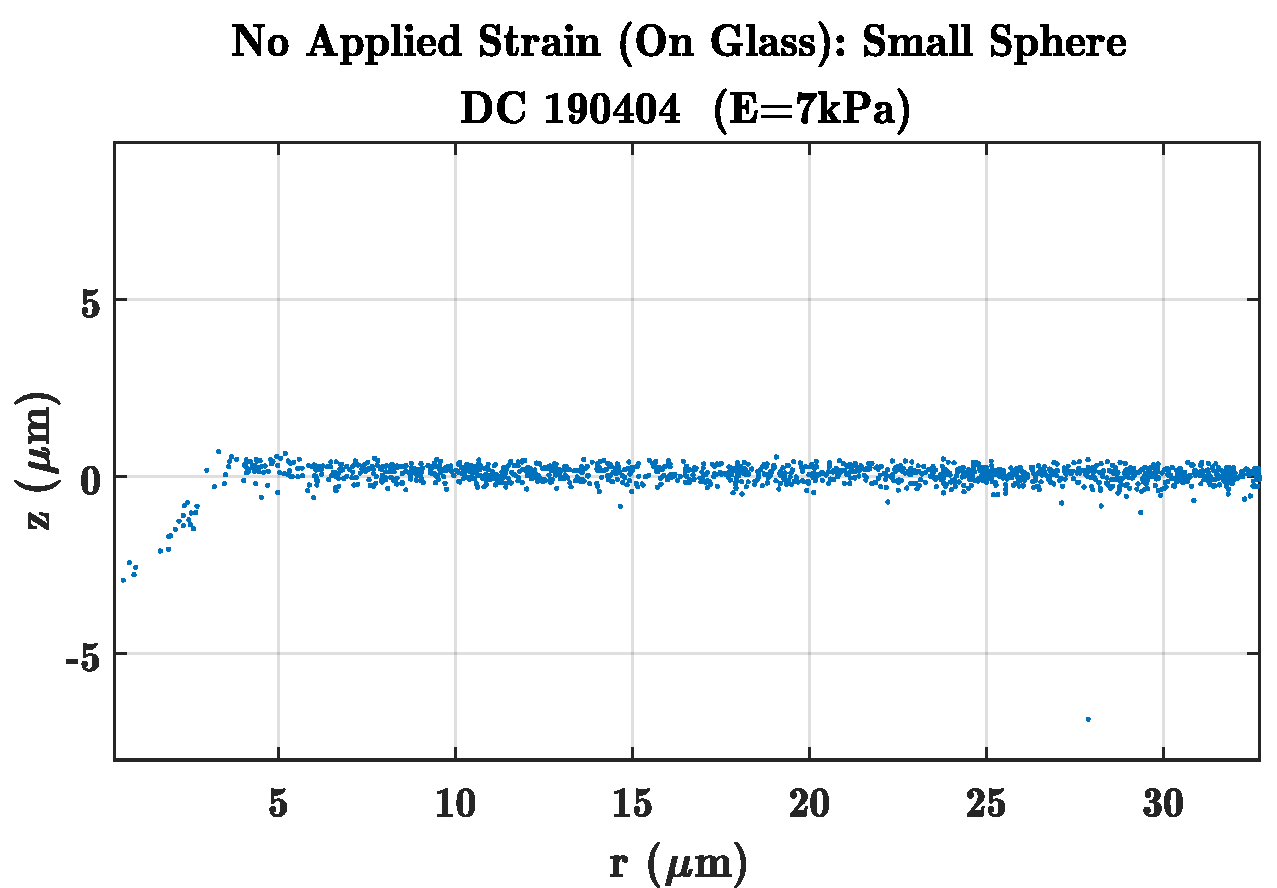
\includegraphics[width=\linewidth]{Chapters/Figures/smallsphere017_190404_DC_glass}
	\caption[Small Sphere Side Profile]{The collapase side profile for small spheres has fewer fluorescent tracer particles to outline there sphere. There is often a cutoff if the sphere sinks in deeper than its ``waist.''}
	\label{fig:smallsphere017190404dcglass}
\end{figure}
\begin{figure}[h!]
	\centering
	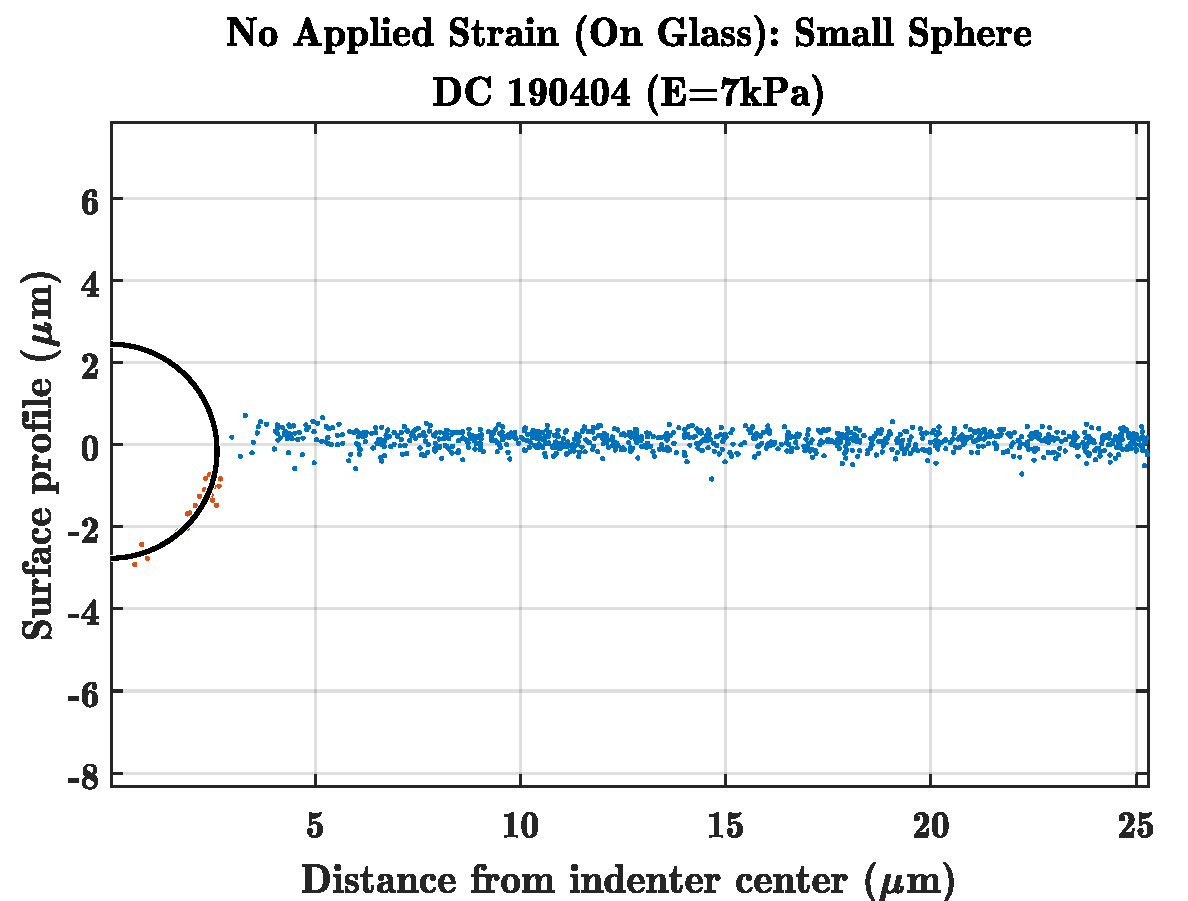
\includegraphics[width=\linewidth]{Chapters/Figures/smallsphere017_cicle_fitsphere_DC}
	\caption[Small Sphere Circle Fit]{For a small sphere where d>r, there is generally a break in the sphere outline. For these circle fits, only the fluorescent beads up to the break are taken into account for the fit.}
	\label{fig:smallsphere017ciclefitspheredc}
\end{figure}


\begin{figure}[h!]
	\centering
	\large \textbf{No Applied Strain (On Glass): Large Sphere}\\ \vspace{.4em}
	\large \textbf{Gelest 9:1 (E=6.3kPa)}
	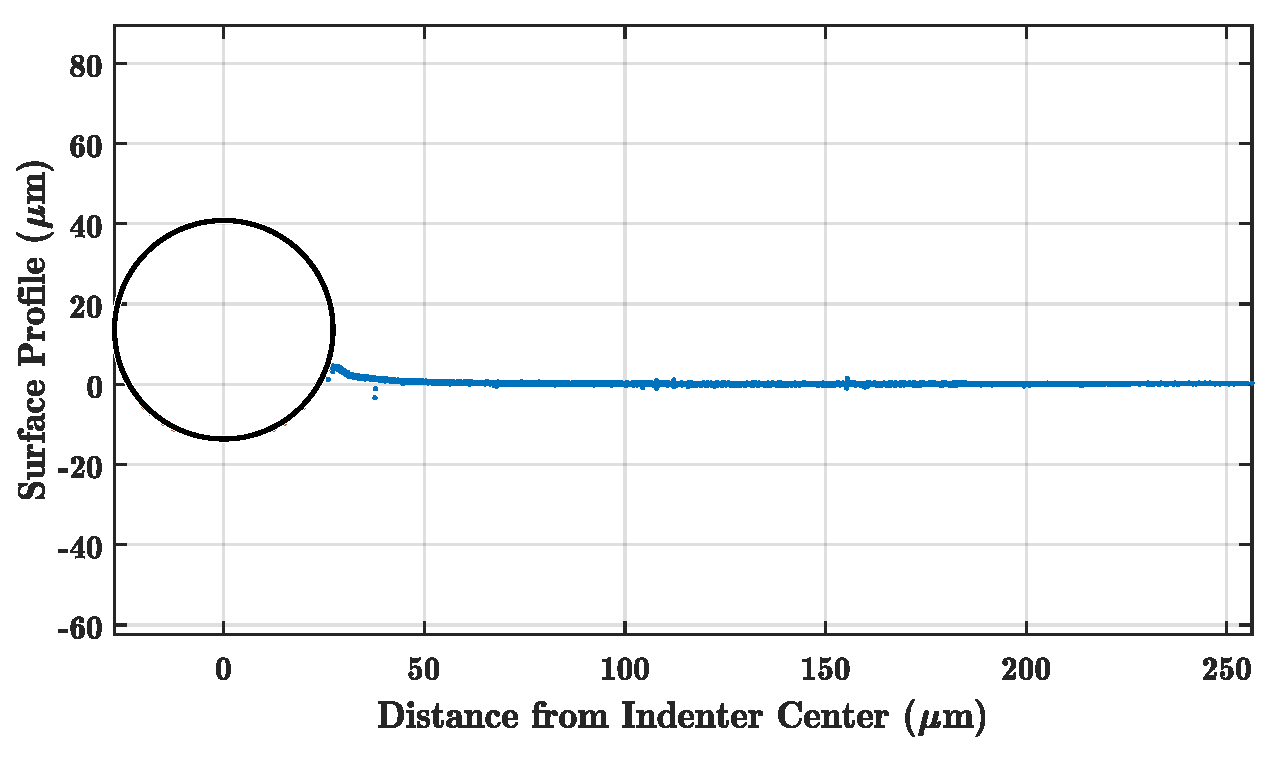
\includegraphics[width=\linewidth]{Chapters/Figures/sphere011_ia/circle_fit}
	\caption[Circle Fit]{This is figure \ref{fig:sidecollapsed}, only with a circle fitted to the indentation sphere. Notice how the surface plane is completely flat and centered at a depth of 0.}
	\label{fig:circlefit}
\end{figure}
\begin{figure}[h!]
	\centering
	{\large \textbf{No Applied Strain (On Glass): Large Sphere}}\\ \vspace{.4 em}
	{\large \textbf{Gelest 9:1 (E=6.3kPa)}}
	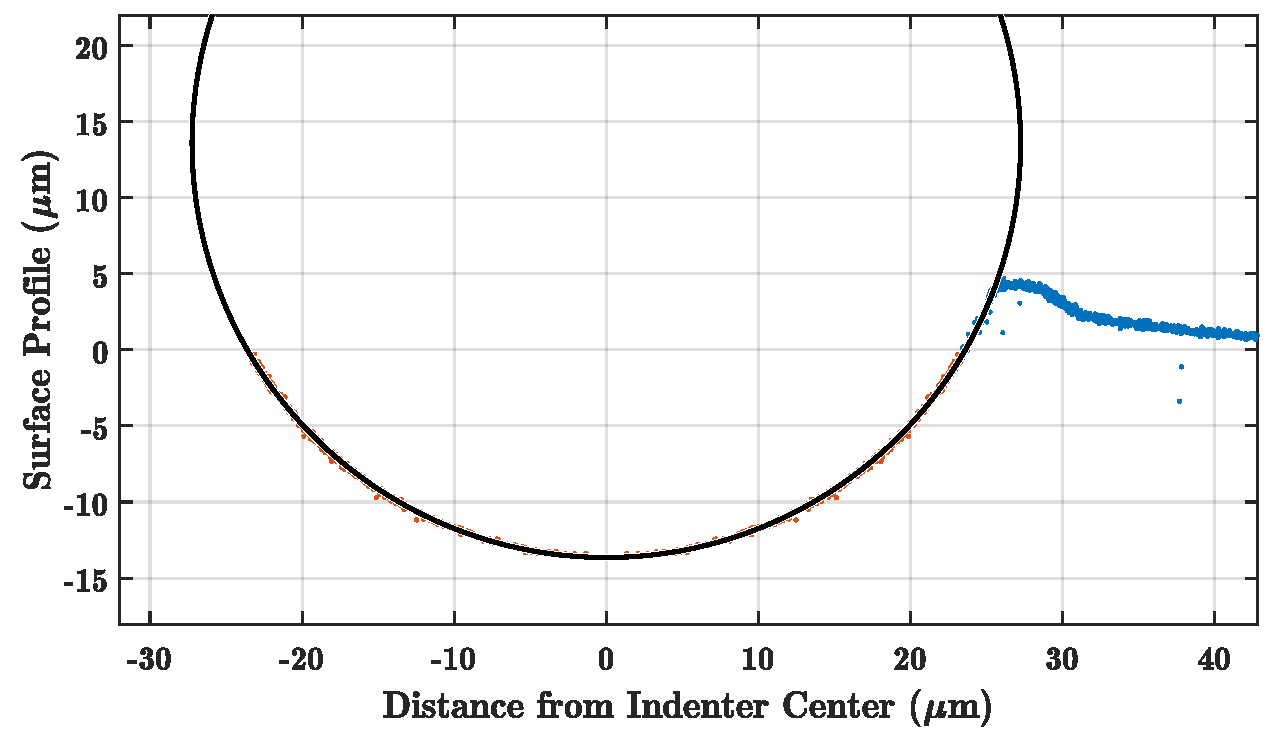
\includegraphics[width=\linewidth]{Chapters/Figures/sphere011_ia/circle_fit_zoomed}
	\caption[Circle Fit Zoomed]{This is simply a zoomed in version of Figure \ref{fig:circlefit}. The orange dots are the data points being used to fit the circle. Notice how the sphere fits nicely in the indentation all the way up to the cusp, past the points being used for the fit.}
	\label{fig:circlefitzoomed}
\end{figure}

After fitting the circle to the substrate's side profile, we can add the depth vs the radius. The radius of the sphere is obviously just the radius of the circle, and the depth is the lowest point of the circle in the z-plane, which we center at $ x=0 $ in Figures \ref{fig:circlefit} and \ref{fig:circlefitzoomed}.  

\begin{figure}
	\centering
	{\large \textbf{No Applied Strain (On Glass): Large Sphere}}\\ \vspace{.4em}
	{\large \textbf{Gelest 9:1 (E=6.3kPa)}}
	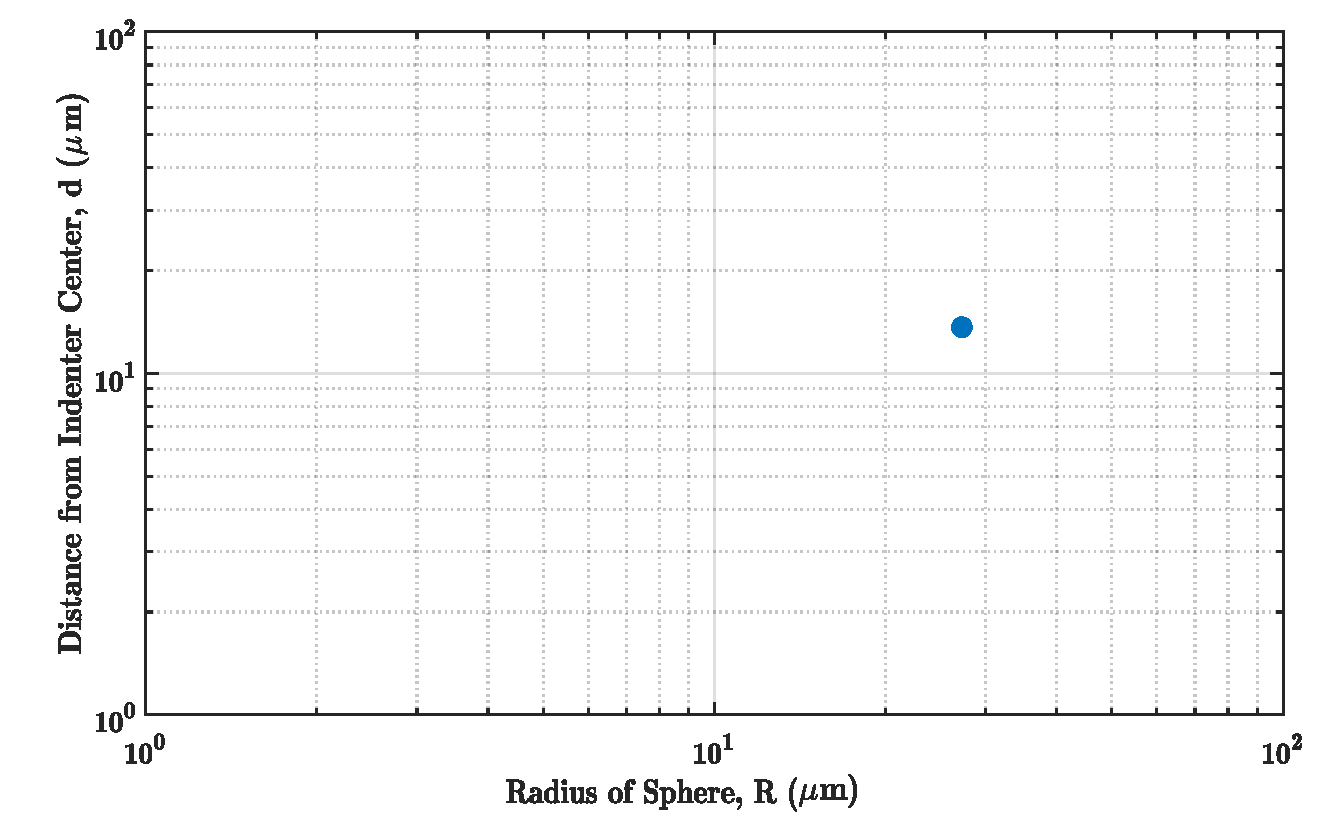
\includegraphics[width=\linewidth]{Chapters/Figures/sphere011_ia/single_d_vs_r}
	\caption[D vs R plot]{All the above analysis leads to this single point, the depth, $ d $ vs. radius $ r $ for a given sphere. By repeating this process for many spheres of varying size, we can fill out the plot and fit equation \ref{THEeqn} to the points. Examples of these fits can be found in Chapter 4.}
	\label{fig:singledvsr}
\end{figure}


\chapter{Surface Stress and Adhesion Results}
In this chapter I present preliminary surface stress and adhesion energy data collected for two types of silicone with various stiffnesses. We first used Gelest to obtain our preliminary data and tune the operation of our device. We then switched to Dow-Corning to continue more extensive measurements. First we give a brief background of the materials used. 


\section{Organosilicon Polymer Chemistry}
\label{section:polychem}
PDMS, or Poly-Dimethyl-Siloxane, is a commonly used polymer gel in the field of soft condensed matter. The gel is composed of a polymer network connected by crosslinkers, with additional free polymer in the fluid phase. When stretched, the large number of covalent bonds resist deformation on a macroscopic level.\footnote{PDMS consists of covalent crosslinkers, however, many compliant materials are a result of physical crosslinkers (e.g. gelatin). When physical crosslinkers are stretched,the configuration of the system changes such that the tangled crosslinkers begin to unwind and untangle. From a statistical mechanics perspective, this decreases the configurational entropy, thus increasing the free energy \cite{Andreotti2020}.} 

%physical crosslinkers: add to ch1 brief descriptions.
%When stretched, the configuration of the system changes such that the tangled crosslinkers begin to unwind and untangle. From a statistical mechanics perspective, this decreases the configurational entropy, thus increasing the free energy. 

Below (Fig. \ref{fig:DMS-V31}) is the chemical structure for the vinyl-terminated PDMS (Gelest) that comprises the fluid phase. 
% Set chemical bonds length
\setatomsep{20pt}

% -------------From chemfig manual, useful macro--------------------
\newcommand\setpolymerdelim[2]{\def\delimleft{#1}\def\delimright{#2}}
\def\makebraces(#1,#2)#3#4#5{%
	\edef\delimhalfdim{\the\dimexpr(#1+#2)/2}%
	\edef\delimvshift{\the\dimexpr(#1-#2)/2}%
	\chemmove{
		\node[at=(#4),yshift=(\delimvshift)]
		{$
			\left\delimleft
			\vrule height\delimhalfdim depth\delimhalfdim width0pt
			\right.
			$};
		\node[at=(#5),yshift=(\delimvshift)]
		{$
			\left.
			\vrule height\delimhalfdim depth\delimhalfdim width0pt
			\right\delimright_{\rlap{#3}}
			$};
	}%
}

%PDMS DMS-V31 Figure
\begin{figure}[h!]
	\centering
	\scalebox{1.75}{
		\setpolymerdelim()
		
		\chemfig{H_2C=C(-[-3]H)--[@{op,0}]Si(-[2]CH_3)(-[6]CH_3)-O--[@{cl,0}]Si(-[2]CH_3)(-[6]CH_3)-C(-[7]H)=CH_2}
		
		\makebraces(20pt,20pt){$\!\!n$}{op}{cl}
	}
	\label{fig:DMS-V31}
	\caption[DMS-V31]{Divinyl-terminated Polydimethylsiloxane (DMS-V31)}
\end{figure}
\noindent The crosslinker for the system is a trimethylsiloxane terminated 25-35\% methylhydrosiloxane - dimethylsiloxane copolymer. The crosslinker is much shorter on average than the PDMS, containing roughly 20-30 repeating monomer groups. The single hydrogen on the methylhudrosiloxane is weakly bound, and can be replaced by one of the hydrogen atoms in the PDMS. This bonding happens over and over again, creating the long twisted chains that create the mesh network of the gel. Increasing density of crosslinkers provides an easy and controllable method to vary the gel's stiffness \cite{Andreotti2020}.

%PDMS Crosslinker HMS-301 Figure
\begin{figure}
	\centering
	\scalebox{1.75}{
		\setpolymerdelim()
		%the [@{op,offset}] and [@{cl,offset}] are for the giant parentheses macro function.
		\chemfig{H_3C-Si(-[2]CH_3)(-[6]CH_3)-O--[@{op,0}]Si(-[2]H)(-[6]CH_3)-O-[@{cl,.5}]-[@{op2,.5}]Si(-[2]CH_3)(-[6]CH3)-O--[@{cl2,0}]Si(-[2]CH_3)(-[6]CH_3)-CH_3}
		
		\makebraces(20pt,20pt){$\!\!m$}{op}{cl}
		\makebraces(20pt,20pt){$\!\!n$}{op2}{cl2}
	}		
	\label{fig:HMS-301}
	\caption[HMS-301]{Trimethylsiloxane terminated 25-35\% methylhydrosiloxane ($m$) - dimethylsiloxane ($n$). This is the crosslinker.}
\end{figure}

\begin{table}[h!]
	\begin{center}
		\begin{tabular}{|c||c||c|}
			\hline
			Mix Ratio (A:B) & Young's Modulus (kPa) & Sol Fraction (\%)\\
			\hline
			$7.5:1$ & $2.5 \,\pm\, 0.1$ & 65.2\\
			\hline
			$9:1$ & $5.0 \, \pm\, 0.1$  & 64.7\\
			\hline
			$11:1$ & $10.0 \,\pm\, 1$  & 63.7\\
			\hline
		\end{tabular}
	\end{center}
	\label{tab:recipes}
	\caption[PDMS ratios Characterization]{PDMS gel characterization for Gelest DMS-V31. By varying the relative density of the crosslinkers, one can predictably control the stiffness of the gel.}
\end{table}




\subsubsection{Silicone Preparation and Spin Coating}\todo[inline,color=pink]{Need to make sure this isn't too repetive for the ch2 section.}
Before spin-coating it is useful to coat the base with fluorescent beads to help determine the substrate's thickness. The only information obtained by this coating is the location of the substrate's bottom surface, so a dense bead coverage is not required, and could potentially be harmful if there is significant light bleeding\footnote{When photons from the fluorophores are bright enough, they are detected in the adjacent images in the vertical stack}. We coat the base (either glass or PDMS) with 40nm beads for 30 seconds - 1 minute. Full directions for preparing a fluroescent bead solution can be found in Appendix B. After this time, we return the fluorescent beads back to the solution for re-use. A significant number of beads will remain on the base, however. To remove some excess, we gently wash the substrate with de-ionized water. For a coverslip, we simply submerge the entire slip in water and gently remove it at a 45\degree angle, using surface tension to prevent the water from breaking-up into smaller droplets. This process is slightly more difficult for the petri dish due to the larger size. We have had success using a container of water with a large opening. Generally, we have used a 1000mL beaker tilted at an angle. It is also possible to use an autopipet for washing - simply repeat the same process used for the fluorescent bead coating, only use water this time. We have had mixed success with this technique, however, as it leaves a water droplet on the surface and often creates an uneven coating of fluorescent beads which manifests itself as streaks across the surface.

After the first layer of fluorescent beads is coated, it is time to spin coat the soft substrate. We aim to make our spin-coated substrates around 100 $\mu$m, and generally spin them to be between $80-100$ $\mu$m thick. Depending on the silicone, we wait a different amount of time before spin coating onto the prepared base, so that the curing process can increase the silicone's viscosity enough to remain on the base when spun. As an extreme examp. We coat our substrate onto coverslips for ``zero applied strain'' data or ont\todo[color=orange]{INSERT THICKNESS SPECS} PDMS sheets from SMI for stretching data.  le, consider trying to spin-coat water; it would all fling off the base. Gelest 9:1 cures rapidly at room temperature, so no waiting time necessary; For Dow Corning 1:1, we wait 45 minutes - 1 hour after combining parts A and B before spin-coating.

To help with the evenness of the coating, we degas the gel by leaving it in a vacuum chamber for a few minutes. A few small bubbles are not of concern, as the process of transferring the gel to the underlayer is enough to pop any remaining stragglers. We have found that a ``glob'' of gel roughly half the diameter of the underlayer, with the spin-coater set to 500 rpm for 40 seconds, is enough to create an even coating of roughly 100 $\mu$m for both Gelest 9:1 and Dow-Corning 1:1 PDMS.

Coating a coverslip with silicone is a straightfoward process where hardly anything can go wrong. Coating the stretchable PDMS underlayer, however, requires some creativity to find the steps necessary to return the best results. I cut the PDMS disk with an X-acto knife and using a standard Petri\todo[color=pink]{ ...double check} dish (2.5in diameter) as a template. In order to avoid snagging, we cut out the circle before removing the paper sheets on both sides of the silicone. Taping the Petri dish to the paper is also helpful prevent the dish from slipping while cutting. Unlike the glass coverslip, the PDMS underlayer is not rigid and must be place on a ridgid surface, such as a Petri dish, for spin coating. This leaves the possibility for air bubbles to become trapped in between the PDMS and the Petri dish. This is a surefire way to ensure an unevenly coated substrate. To avoid this, we remove the top paper sheet of the newly cut PDMS, then place the Petri dish down upon the exposed silicone. This creates dish with a silicone disk on top and a paper sheet on top of that. We then push all the air bubbles out from the center outwards with out thumbs. Finally, any tiny air bubbles can hopefully be removed by placing the Petri dish in a vacuum chamber for a few minutes. It is at this point that we coat the PDMS with fluorescent beads and wash as desired before placing the petri dish onto the spin-coater and proceeding as described above.

After spin-coating, the silicone requires time to cure. We cure Dow-Corning 1:1 for at room temperature for at least 24 hours. For Gelest 9:1, we oven cure at $70 \degree$ C for at least 24 hours. Either silicone can be cured at room temperature or in the oven so long as a sufficient amount of time is waited, however, we have used this methods to maintain consistency, as well as parallel the techniques used in previous literature \cite{xu2017direct}.

After the silicone cures, we coat the surface with fluorescent beads again. It is important that the beads are dense enough to give a high resolution, yet not so dense as to become indistinguishable. For the 40nm bead solution prescribed in Appendix B, we allow the solution to soak for up to 1.5 minutes before removing and washing the substrate. While the fluorescent beads chosen are most susceptible to light at 440 nm, there is still the risk of photo-bleaching the fluorophores, and it is worth dimming the lights in the lab when working with them. 

\section{Preliminary Data: Gelest}
Because Figure \ref{fig:2017natcomfig} was obtained using Dow-Corning silicone gel, our intention from the start was to use this material in our adhesion based measurements. Because the material was back-ordered, we used Gelest instead while we calibrated the process. I present this preliminary data because it shows clear incremental steps of evidence that the surface stress for the substrate is increasing under strain.  

\subsection{Standard Candles}
Not only do we measure the depth and radii for a range of spheres, but we also measure a select few spheres at every strain. This allows us to track how any given sphere is changing, increasing our confidence that the shift in $\Upsilon$ and W is not just an artifact of noise. Below is the side profile for Gelest 9:1 ($\text{E}=6.3$ kPa). Notice how the profile shifts noticeably upwards to be flattened when the substrate is stretched. This shift is expected if the surface stress is increasing (see equation \ref{THEeqn}).

\begin{figure}[h!]
	\centering
	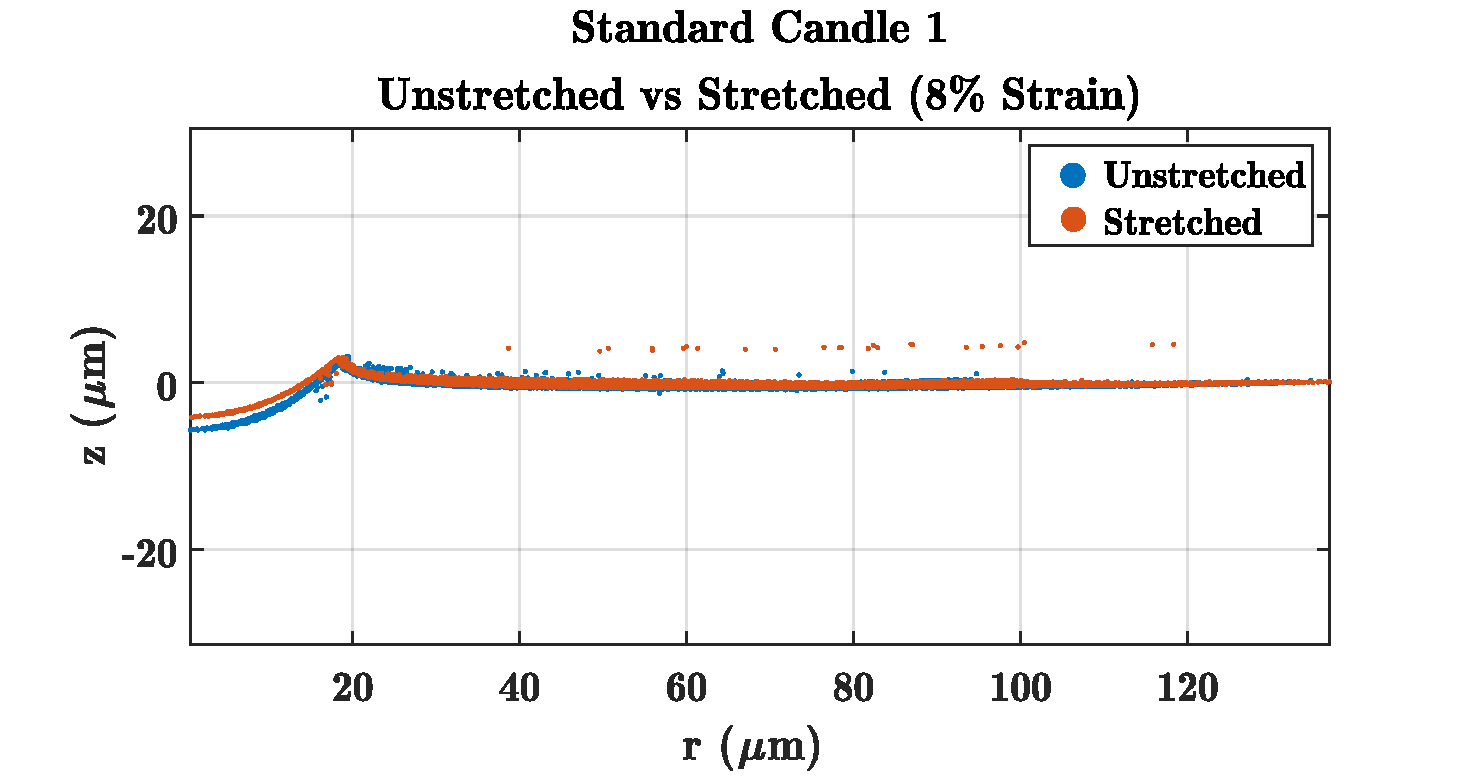
\includegraphics[width=\linewidth]{Chapters/Figures/sc1_unstretched_v_8ml}
	\caption[Side Collapse Comparison]{The side profile of the same sphere before and after stretch. Notice how after stretching, the sphere's indentation into the substrate is shallower. Substrate is Gelest 9:1 ($\text{E}=6.3$ kPa).}	
	\label{fig:sc1unstretchedv8ml}
\end{figure}

There is a lot of noise for D vs. R data collected with substrates on our stretching apparatus have a lot of noise. As seen in figure \ref{fig:glassvsstretched190218}, the D vs. R data collected on glass is far cleaner than that collected on the stretcher when strained. We can see the trend that under strain, the spheres sink into the substrate less deep. At 22\% strain, we expect zero strain-stiffening of our elastic substrate, and conclude that this change in depth is a result of an increase of surface stress, $ \Upsilon $. Unfortunately, the d vs. R values are too noisy/scattered to make a reasonable fit to extract $ W $ and $ \Upsilon $ values.

\begin{figure}[h!]
	\centering
	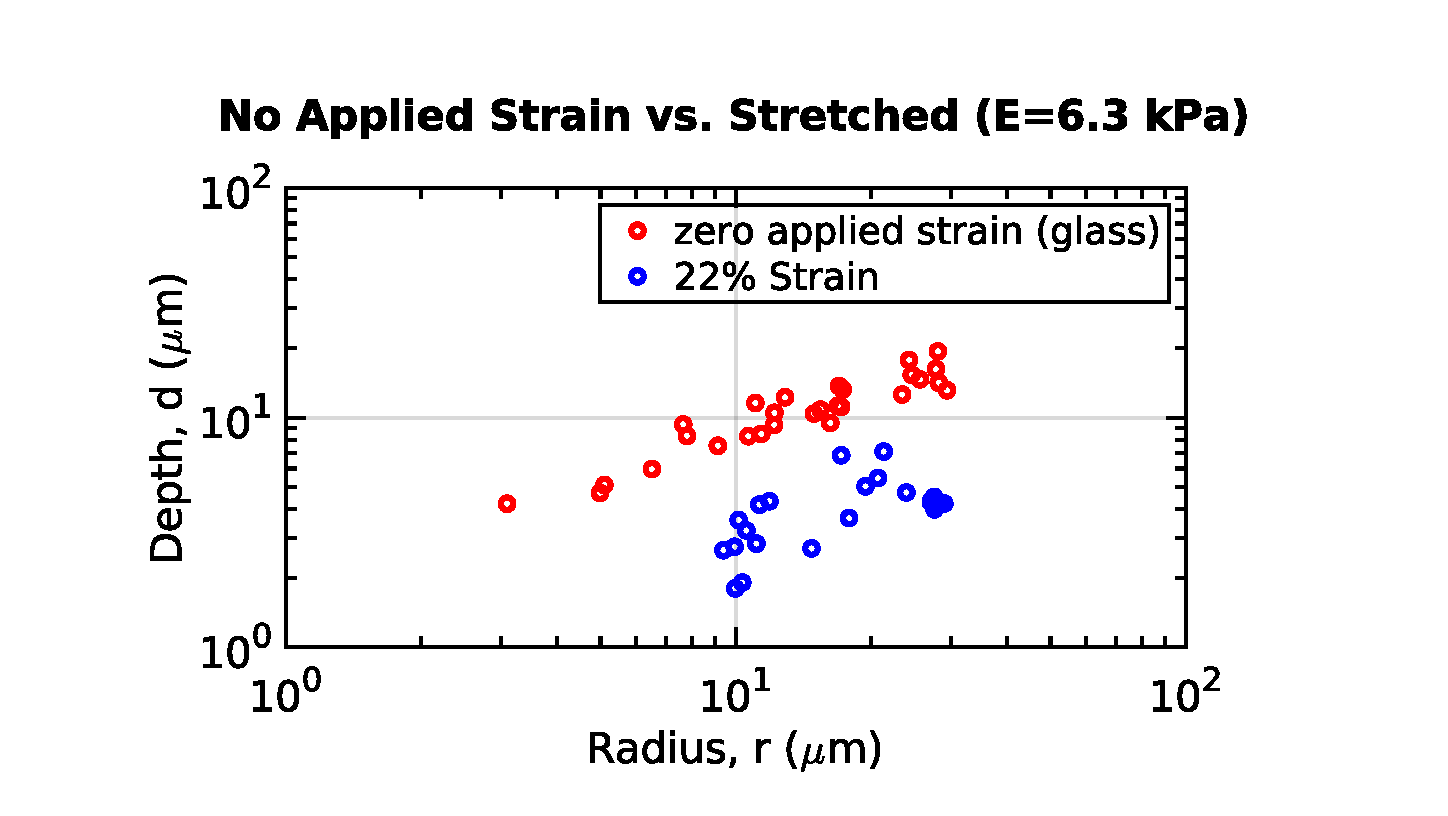
\includegraphics[width=\linewidth]{Chapters/Figures/glass_vs_stretched_190218}
	\caption[Glass vs. Stretched d vs. R]{For Gelest 9:1, the silicone under strain (blue) on average sinks less deep into the silicone than for the same silicone spun on glass (zero applied strain). The large noise for the strain-data meant we could not meaningfully determine $ \Upsilon $ and $ W $ to measure the variation in $ \Upsilon(\epsilon)$ and $W(\epsilon)$. \emph{COME BACK TO THIS AND FIX THE PLOT TO MAKE IT MATCH THE OTHERS}}
	\label{fig:glassvsstretched190218}
\end{figure}

\begin{figure}[h!]
	\centering
	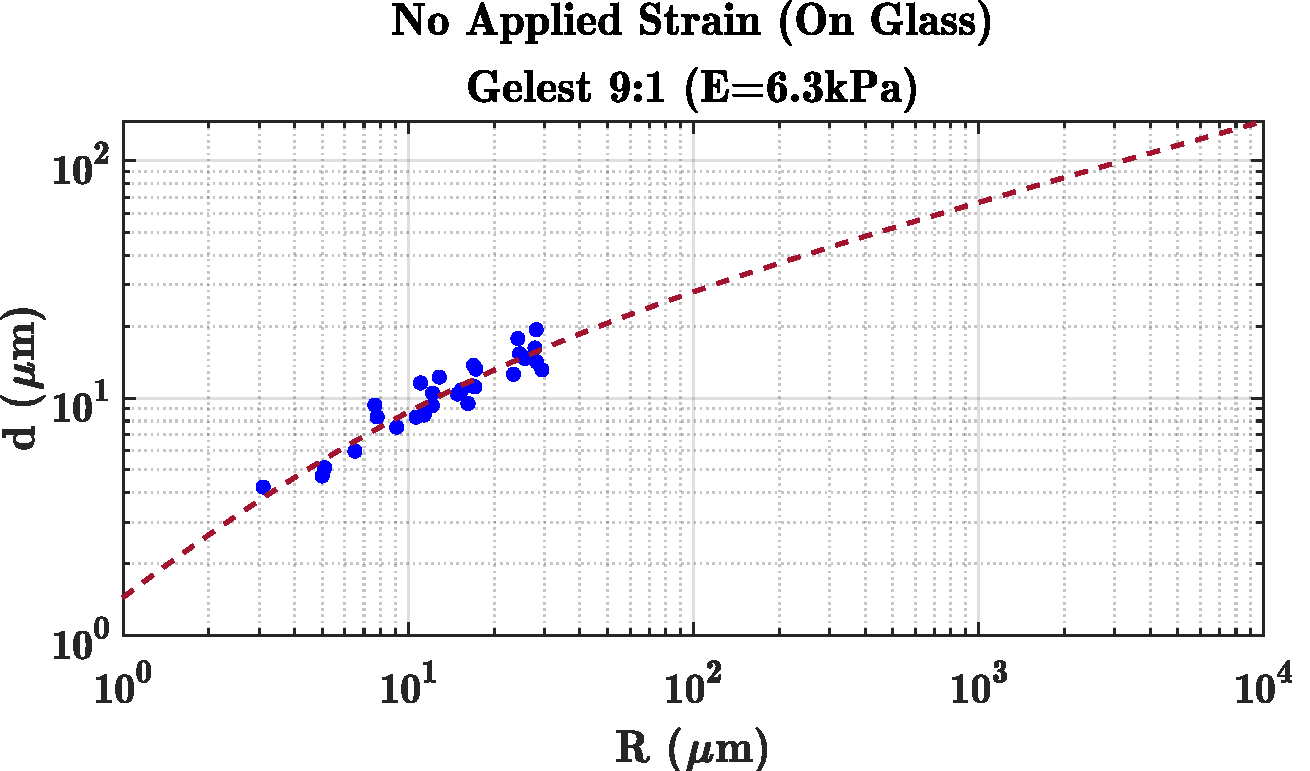
\includegraphics[width=\linewidth]{Chapters/Figures/w_ups_fit_G9-1}
	\caption[Gelest W-$\Upsilon$ Fit]{We fit Equation \ref{THEeqn} to the d vs. R plot for a Gelest 9:1 sample. The best fit line returns parameters of $ W=53 $  and $ \Upsilon=32 $ mNm$^{-1}$.}
	\label{fig:wupsfitg9-1}
\end{figure}

\section{Dow-Corning PDMS}
Because the $ \Upsilon(\epsilon) $ measurement in \textit{Nature Communications} 2017 \cite{xu2017direct} was conducted using a Dow-Corning PDMS substrate, we are especially interested in using this material for our $ \Upsilon(\epsilon) $ measurements. Because there has only been one measurement of $ \Upsilon(\epsilon) $ in soft matter, in order to have value to use as comparison, we need to use use the same material. 

Our first measurements with Dow-Corning PDMS returned largely varying results; the stiffness of the silicone varied by a factor of 2 from the expected value, and the stiffness continued to increase as the silicone cured over a period of several weeks, as opposed to the usual 24hr time-frame. Furthermore, the adhesion of the PDMS varied from sample to sample. Often the silica sphere would not adhere to the surface. It was eventually discovered that the Dow-Corning PDMS being used expired several years prior. Some of the measurements conducted, however, returned results of interest, and thus have been included here. 


\begin{figure}[h]
	\centering
	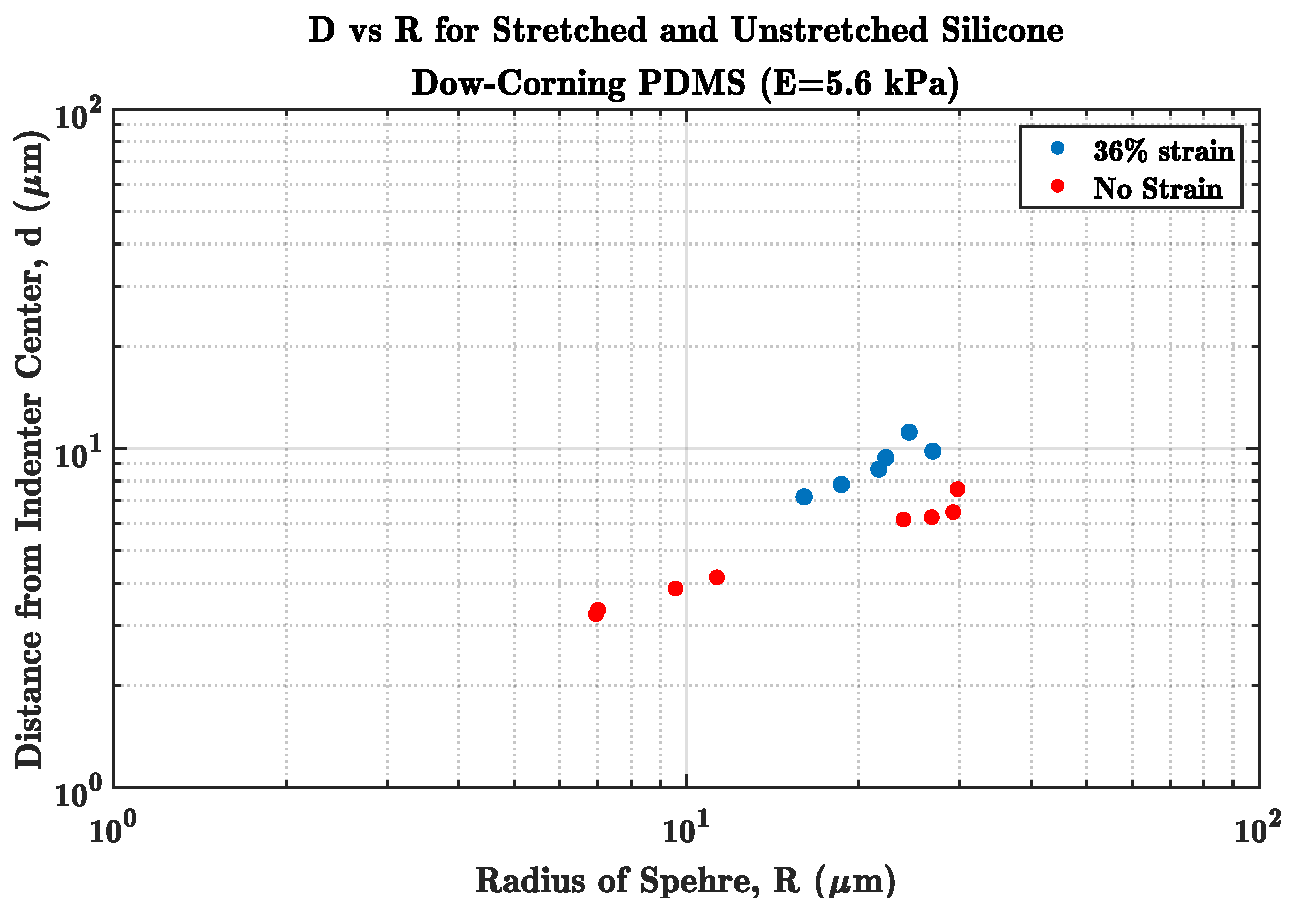
\includegraphics[width=\linewidth]{Chapters/Figures/d_vs_r_stretch_vs_no_stretch_DC181115}
	\caption[D vs. R Dow-Corning]{Here we plot D vs. R for a Dow-Corning PDMS Substrate at two different strains. Notice how at higher strains, the spheres sink in less deep. This can be explained by an increase in $\Upsilon$ or an increase in $E$ for the substrate.}
	\label{fig:dvsrstretchvsnostretchdc181115}
\end{figure}

\begin{figure}[h]
	\centering
	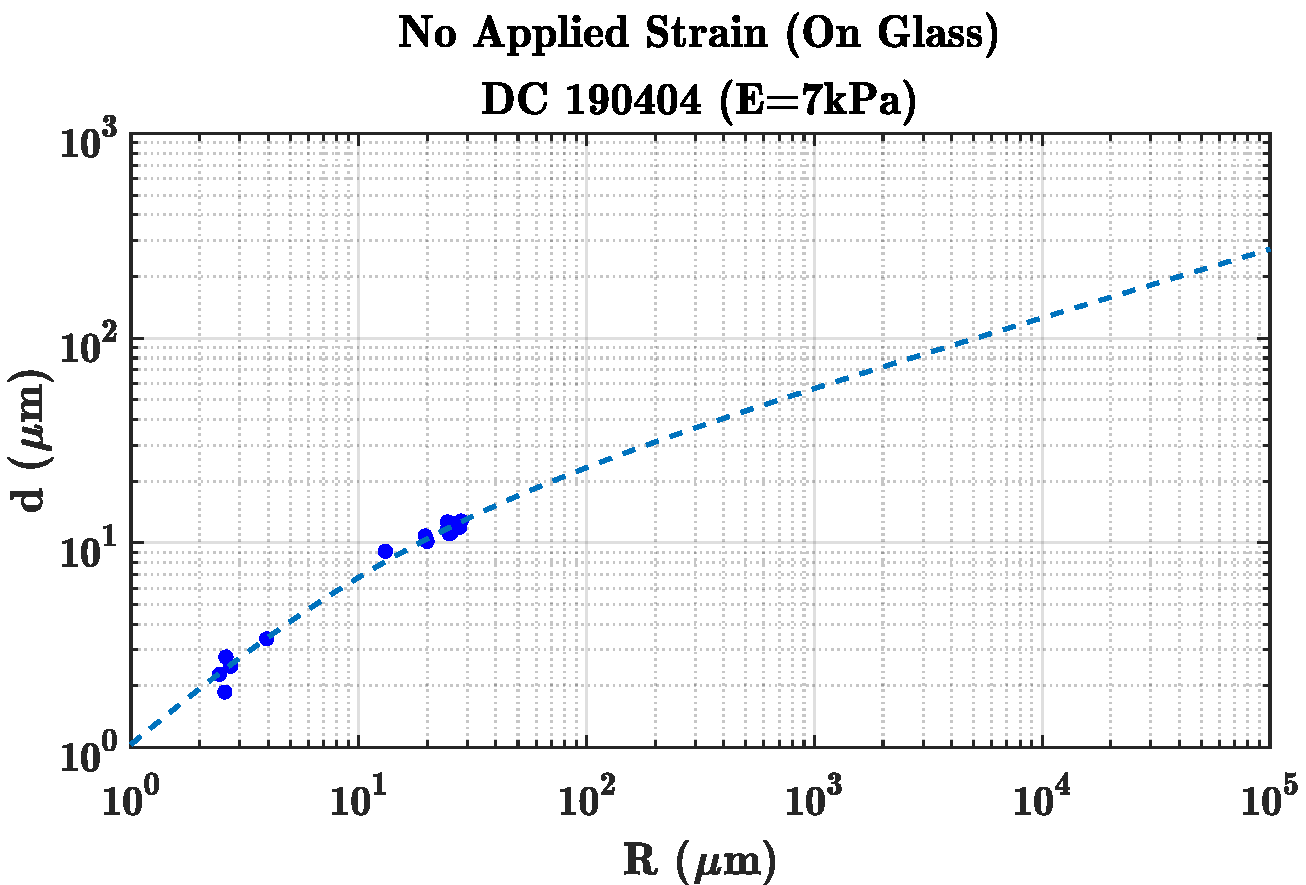
\includegraphics[width=\linewidth]{Chapters/Figures/WUps_fit_DC190404}
	\caption[Dow Corning W-$\Upsilon $ Fit]{The surface stress and adhesion energy fit for Dow Corning PDMS silicone with no applied strain. Given the d vs. R values, the fitting parameters to make the best fit line are W $ = 48.6$ and  $\Upsilon = 43.5$ mNm$^{-1}$.}
	\label{fig:wupsfitdc190404}
\end{figure}

\todo[inline,color=pink]{TexStudio broke the figures and writing up weirdly. Will fix later. Also, I have a stretchable Dow-corning substrate ready to go. I'd like to take this $ \Upsilon(\epsilon) $ measurement next week.}

\chapter{Future Work}
\section{Noise Minimization}
As covered in the previous chapter, the limiting factor for our $ \Upsilon(\epsilon) $ and $ W(\epsilon) $ measurements is the noise present for all d vs. R data collected on stretchable substrates. We believe this noise is a result of the uneven mount that holds the stretching apparatus on the microscope's stage. We have corrected the mount's tilt by sanding and re-gluing the sides of the mount; however, if this does not correct the tilt, there are still options to consider. 

If the mount is still too uneven, we could put tiny piezoelectric step motors on three corners of the mount, allowing for precise leveling of the surface plane for each sphere during data collection. We believe this will not be necessary, however, and suspect the reduced tilt from its current state will be sufficient to level the surface plane in post via software.

Alternatively, we have been measuring the radius of the spheres by fitting a circle to the azimuthal collapse, or side profile (see Figure \ref{fig:circlefitzoomed}). Instead, we could fit a sphere to the three-dimensional indentation (such as Figure \ref{fig:particlelocatednormalized}). The advantage of fitting a sphere rather than a circle would be the increased number of points used for the fitting. We do not suspect the circle-fitting used for measuring $ R $ has been contributing to the noise observed. However, this spherical fitting technique may be useful in measuring r for very small spheres, which have been problematic for the circle fits.    


\section{New Materials}
The adhesion based technique for measuring $\Upsilon(\epsilon)$ should be applicable to virtually any soft solid capable of being stretched. Naturally, we would like to expand our measurements beyond silicone. Hydrogels, aerogels, gelatins, and commercial adhesives, to name a few, are materials of interest. 
\subsection{Neue Materialen: Gummibärli}
Measuring the strain dependent surface stress of a gummy bear presents challenges not present in PDMS silicone. For example, gummy bears come in a predefined size and shape. In order to spin coat them on our apparatus, we must first melt down the gummies. Gummy bears are composed primarily of gelatin and a glucose syrup.\footnote{American gummy bears use corn syrup. However, we are using Swiss  Gummibärli, which likely use a different variety}  When melted, they tend to re-solidify as brittle and incompressible. To resolve this, \todo[color=pink,inline]{chat with KEJ about what Adam's done so far and if we solved this brittleness problem. I think just using a lower temperature would work though}
  
\section{Future Techniques}
Currently, we use equation \ref{THEeqn} to run a two parameter fit for the surface stress, $ \Upsilon $, and the adhesion energy, $ W $. Alternatively, it is possible to measure the adhesion energy separately. This technique, though not critically important to the experiment, is worth exploring. Measuring $ W $ separately and comparing the measured value to the calculated value via the two parameter fit would inform us about the accuracy of our fit for the zero-strain data, and possibly the strain-data if the adhesion energy per area is independent of strain, i.e. $ W = W(\epsilon) $.   



% the \appendix tag tells LaTeX where it should start labeling chapters with letters (denoting appendices) rather than numbers (denoting main chapters)
\appendix 
\chapter[Stretching Apparatus Design]{Stretching Apparatus Engineering Design Documents}
%Appendix
\section{Details of Stretcher Design}

Aluminum was chosen as the base material because of its sturdy yet malleable nature, making it an excellent material with which to mill. Acrylic was considered, but was not chosen because of its brittle nature; we were concerned about cracking when drilling the UNF threads connecting to the Luer-lock syringe.

The stretched sheet is laid over the lubricated apparatus and fixed in place using a 48.7mm diameter by 1.6mm thick rubber O-ring. A removable plastic ring is then placed on top of the o-ring and clamped down using a tension clamp attached to a fitted plastic base slotted for the stretching apparatus to sit. The plastic ring is constructed from an engineering plastic that came from a similar but malfunctioning device used by our colleagues at ETH Zürich. The outer ring could easily be laser cut from a plastic or milled out of aluminum if desired. 

To pull a vacuum, a 1/4-28 UNF to female Luer connects the apparatus to a plastic 100ml Luer-lock syringe. We found a more consistent stretch was held by lining the inner walls of the syringe in more Dow Corning vacuum grease. The UNF to female Luer connector is stainless steal, and coated with Dow Corning vacuum grease. The inclusion of a small o-ring between the UNF threads and the cylindrical base proved critical in holding vacuum for sustained periods of time.

The vacuum pull was controlled by a Harvard Apparatus Elite 11 Syringe Pump. This allows us to have a consistent withdraw rate and control over the amount of air withdrawn down to the pico-liter level, a far ggreater precision than needed. Stretching was found to work best at maximum withdrawal rate. Our stretching apparatus has sustained a constant equibiaxial stretch at 35\% strain for as long as 5 hours. Maximum strain percentage and during of maintained stretch is yet to be fully tested.


\begin{figure}[h!]	
	%\centering centers the figure on the page.  This is convention.

	\vspace{-3.7em}
	\centerline{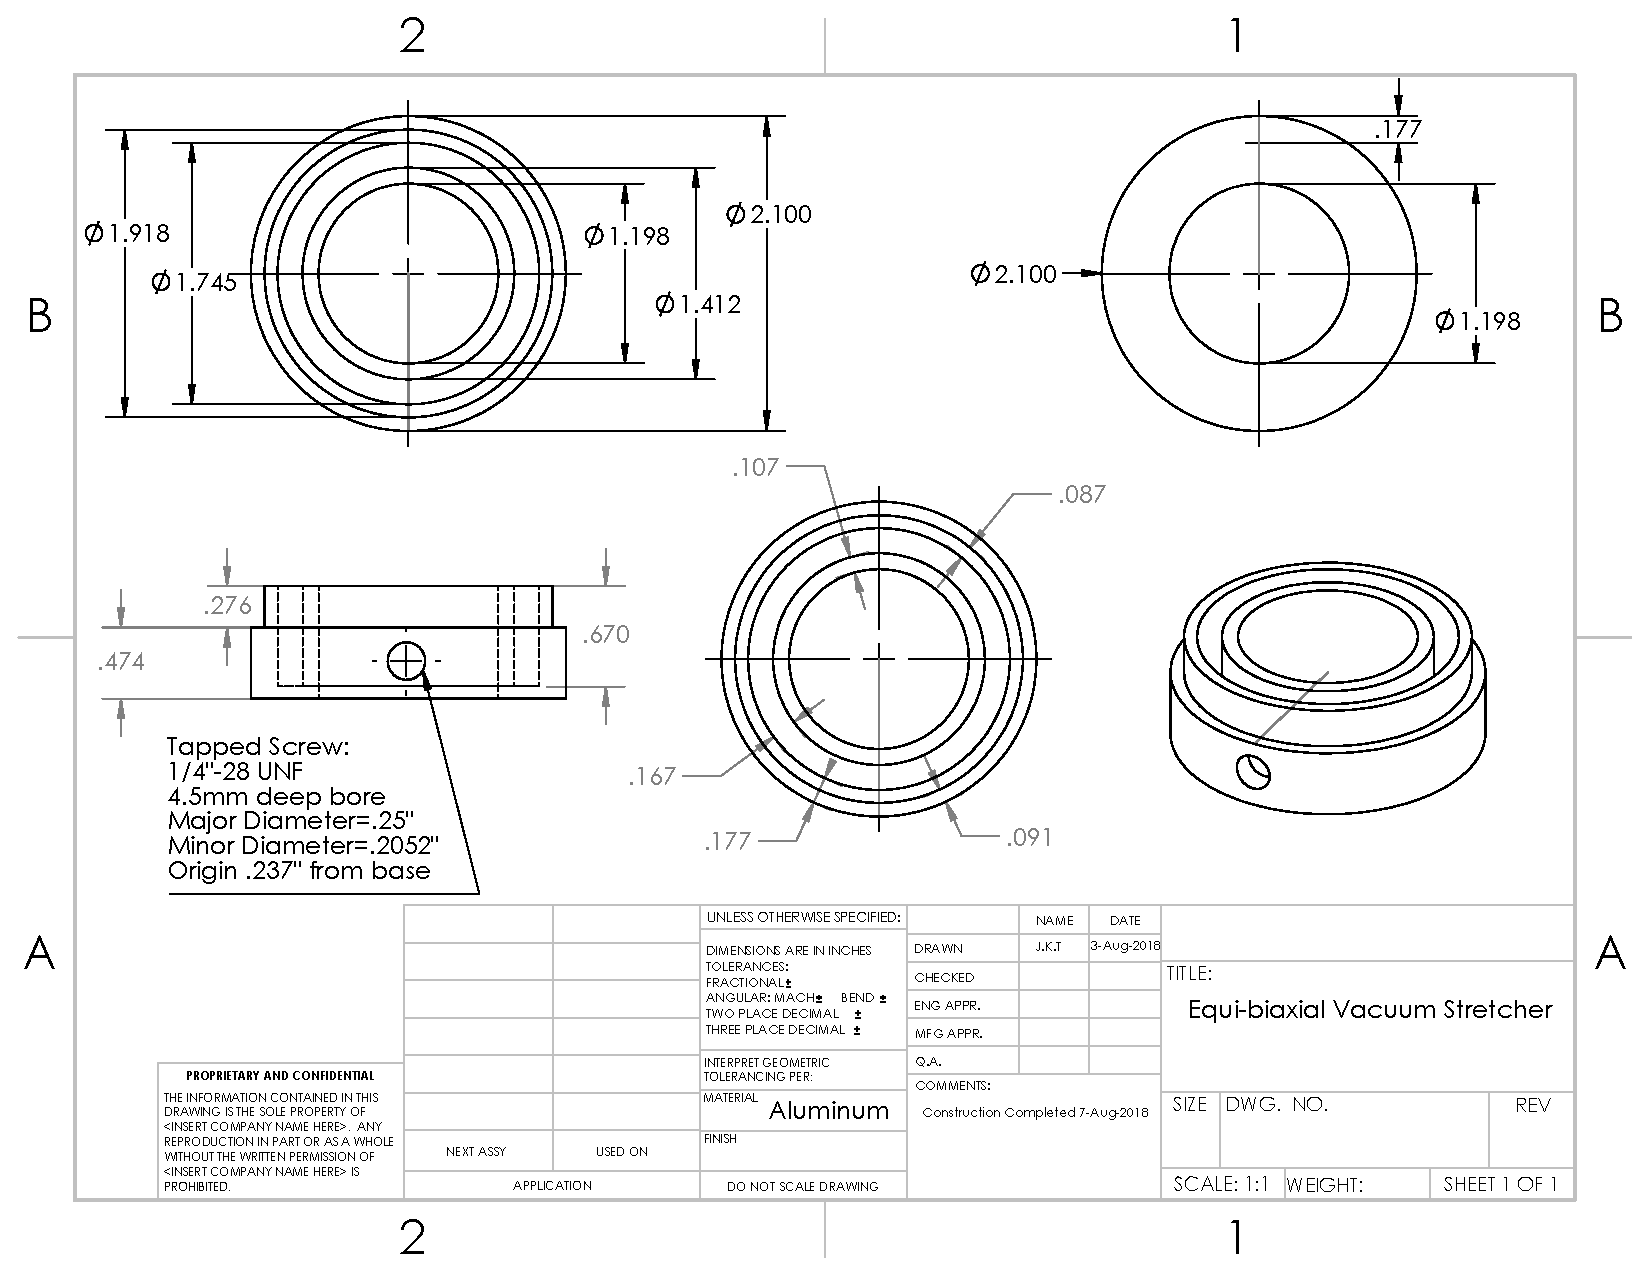
\includegraphics[scale=.65]{Chapters/Figures/Stretcher_body_with_screwtap_updated.PDF}}
	 
	\caption[Stretching Apparatus Design Document]{The equi-biaxial vacuum stretcher design document. Note: all measurements are in inches.}
	
%	This reference can be called in the text using the \ref tag.
	\label{fig:stretcherDesignBase}
\end{figure}


\begin{figure}[h!]
	%\centering centers the figure on the page.  This is convention.
	
	
	\centerline{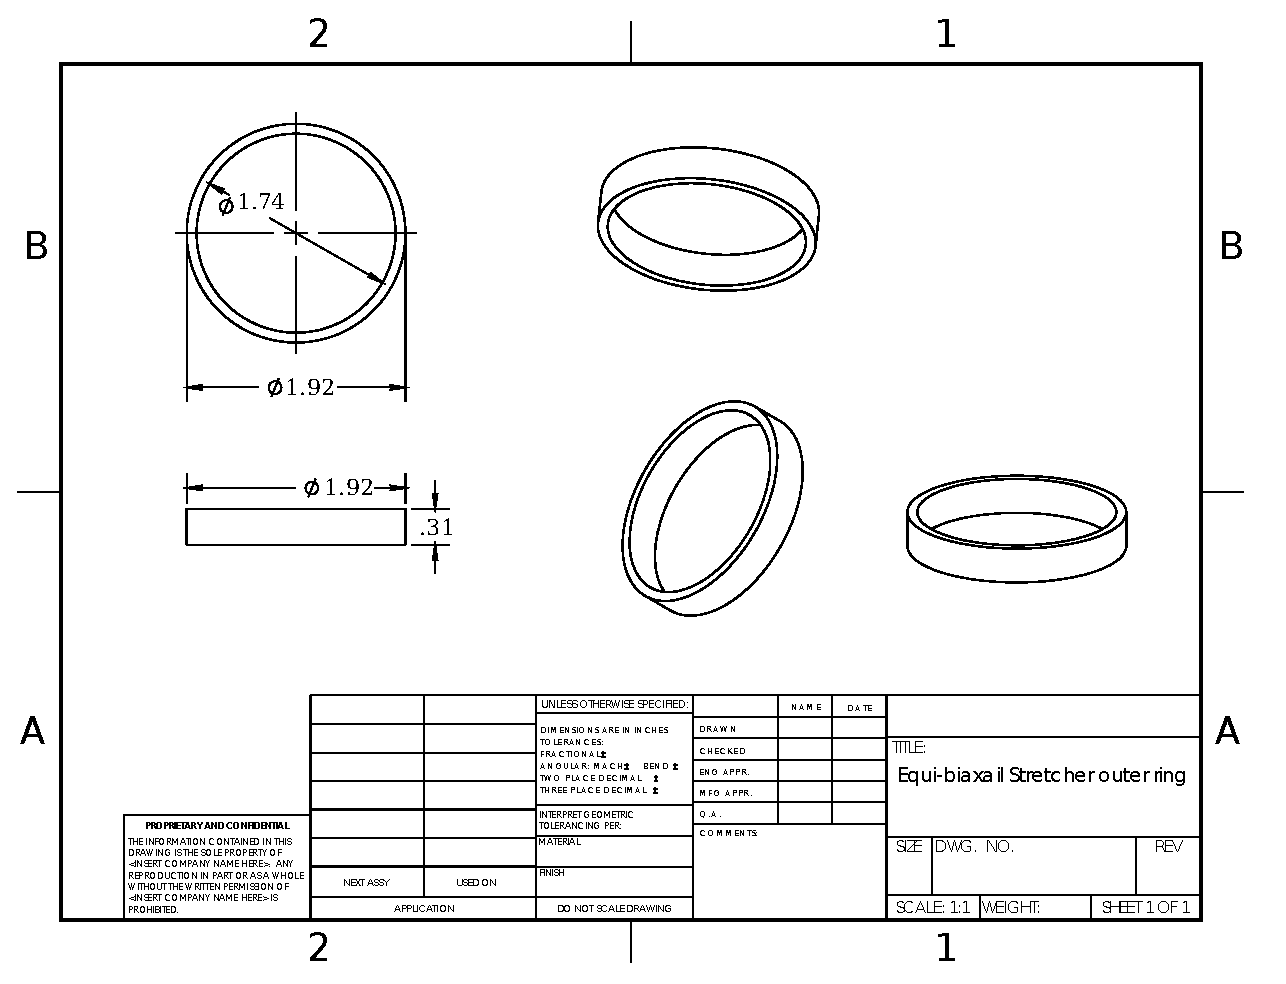
\includegraphics[scale=.85]{Chapters/Figures/Stretcher_outer.pdf}}
	\vspace{-.7em}
	\caption[Stretcher outer-ring]{Engineering Design Document of the outer-ring for the Stretching Apparatus. Note: all measurements are in millimeters.}
	
	%	This reference can be called in the text using the \ref tag.
	\label{fig:stretcherDesignRing}
\end{figure}

%Appendices are a good idea for almost any thesis.  Your main thesis body will likely contain perhaps 40-60 pages of text and figures.  You may well write a larger document than this, but chances are that some of the information contained therein, while important, does \emph{not} merit a place in the main body of the document.  This sort of content - peripheral clarifying details, computer code, information of use to future students but not critical to understanding your work \ldots - should be allocated to one or several appendices.  


%\chapter{Substrate Stiffness Measurement}
%\input{Chapters/Appendix_stiffness}

\chapter{Fluorescent Bead Recipe}
\input{Chapters/Appendix_beads}

\chapter{MATLAB Code}
%appendix3
Below, we list and briefly explain the function of each MATLAB program used in analyzing the raw TIF images.


\def\code#1{\texttt{#1}}

\subsection{Confocal Analysis Codes}
Below I list the MATLAB codes used in analyzing the raw .ome.tif files obtained from the confocal imaging process. I will list them in the order executed to obtain the desired d vs. R values. In each description, I will also include the required files needed to run the script.

\subsubsection*{iterative\_locating\_input\_parameters\_2018.m}
\begin{itemize}
	\item Set particle locating parameters such as estimated particle size, brightness intensity range, and minimum separation
	\item Define the image stack to be analyzed
	\item Rescale the image from pixels to microns
\end{itemize}
\subsubsection*{iterative\_particle\_locating.m}
\begin{itemize}
	\item Locates the fluorescent beads
	\item Returns a .txt file with the locating information and creates a figure 
	\item Produces Figure \ref{fig:particlelocatednormalized}
\end{itemize}
\subsubsection*{process\_and\_collapse\_confocal\_data.m}
\begin{itemize}
	\item Estimate the center point of the sphere in the format of \code{[x,y] + return} using Figure \ref{fig:particlelocatedtopview}
	\item Follow the directions printed on the screen to collapse the side profile of the sphere
	\item Creates Figure \ref{fig:sidecollapsed}
\end{itemize}
\subsubsection*{circle\_fit\_confocal\_profiles.m}
\begin{itemize}
	\item You must edit this script for the first time you analyze a sphere for a given data set.
	\item This script fits a circle to the collapsed side profile
	\item Script saves the d vs r value as a .mat file, adds the \code{[d,R]} data to a list of all \code{[d,R]} values (or creates that list if it's the first time being run for a data set), and plots the d vs. R data
	\item Produces Figure \ref{fig:circlefit}
\end{itemize}

\subsection{Strain Calculation Codes}
The codes used for calculating the strain are credited to Rob Style and Ross Boltyauski
\subsubsection*{master\_tracking\_gui.m}
\begin{itemize}
	\item This program requires many additional scripts, though it has easy to follow directions. Instead, we provide example code for measuring the strain. The final output is 'C', the strain-tensor, and 'T', the displacement vector.
	\item \code{params = master\_tracking\_gui(`sample1\_unstretched.tif')}
	\item \code{params(2) = master\_tracking\_gui(`sample1\_stretched.tif')}
\end{itemize}
\subsubsection*{stretch\_est\_gui.m}
\begin{itemize}
	
	\item Now grab the peak positions out of the data structure:
	\item \code{r = params(1).pks(:,1:2)}
	\item \code{r2 = params(2).pks(:,1:2)}
	\item \code{[A,t] = stretch\_est(r,r2)}
	\item \code{[C,T] = stretch\_refine(r,r2,A,t,2,1)}
	
\end{itemize}



\subsection{Silicone Characterization Measurements}
To measure the stiffness of our silicone (Young Modulus, E), we use the TA XTPlus Texture Analyzer. We measure the force of resistance (N) vs. depth of compression (m) for several points near the center of the bulk, which we export as .txt files. We only use points near the center to isolate the silicone. Measuring near the sides could include the restorative force from the walls of the container.
\subsubsection*{measure\_modulus.m}
\begin{itemize}
	\item Calculates the average slope of this curve. This is the Young Modulus of the substrate.  $(\sigma/\epsilon)$
	\item The requested starting position is the x-axis value where the linear slope approximately begins. It is better to overshoot the starting value than undershoot it
\end{itemize}



% \bibliographystyle tells LaTeX how you want to format your bibliography.  There are many standard formats.  apsrev is fairly typical, but feel free to explore other options if the mood strikes.  
%\bibliographystyle{apsrev}
\bibliographystyle{goodStyle}

% \bibliography calls the actual file that contains your bibliographic information.  This file can be generated by hand or in an automated way using software such as BibTeX.  Either works fine, but it is worth learning to use BibTex in the long term.  Take a look at the .bib file included here if you want to get some idea of the formatting required to create a bibliogrphy file of your own.

\bibliography{bibliography}
\end{document}